\documentclass[11pt,aspectratio=169]{beamer}

\usepackage[T1]{fontenc} % pour le français
\usepackage[utf8]{inputenc}
\usepackage{lmodern}
\usepackage[french]{babel}
\usepackage{graphicx}
\usepackage{hyperref}
\usepackage{xcolor}
\usepackage{amsmath}
\usepackage{csquotes}
\usepackage{caption} 
\usepackage{subcaption} % for subfigures
\DeclareCaptionLabelSeparator{custom}{ -- }
\captionsetup[figure]{labelformat=simple, labelsep=custom, name=Figure}
\usepackage{amsfonts}
\usepackage{listings}
\usepackage[natbib=true,style=authortitle,backend=bibtex,useprefix=true]{biblatex}

% Links to other files
\addbibresource{references.bib}
\graphicspath{{figures/}}


% Beamer template customisation
\beamertemplatenavigationsymbolsempty
\setbeamertemplate{page number in head/foot}[totalframenumber] % numéros de slides
\setbeamercovered{transparent}
\usetheme{Madrid}
\usecolortheme{default}

% Setup colors title page + footline
% \definecolor{deepblue}{RGB}{0, 50, 100} 
\definecolor{deepblue}{RGB}{142, 60, 140} 
\definecolor{roose}{RGB}{226, 0, 122}
\setbeamercolor{title}{bg=deepblue, fg=white} 
\setbeamercolor{frametitle}{bg=deepblue, fg=white}
\setbeamercolor{footline}{bg=deepblue, fg=white}
\setbeamercolor{author in head/foot}{bg=deepblue, fg=white} 
\setbeamercolor{title in head/foot}{bg=deepblue, fg=white} 
\setbeamercolor{date in head/foot}{bg=deepblue, fg=white}

% No more bold font in footline
\setbeamerfont{author in head/foot}{series=\normalfont}
\setbeamerfont{title in head/foot}{series=\normalfont}
\setbeamerfont{date in head/foot}{series=\normalfont} 
\setbeamerfont{footline}{series=\normalfont} 

% To cite papers manually
\newcommand{\manualcite}[1]{\textcolor{gray}{\small[#1]}}

% TITLEPAGE
\author[Gendron \& Guibon]{\large Barbara Gendron-Audebert$^{1,2}$ et Gaël Guibon$^1$ \\ \texttt{\{prénom.nom\}@loria.fr}}
\title[\textsl{Metric learning} pour l'ERC en contexte]{SEC : contexte émotionnel phrastique intégré pour la reconnaissance émotionnelle efficiente dans la conversation \vspace{5pt}}
% \subtitle{\vspace{10pt} Session commune 1 - JEP-TALN 2024}
% \date[JEP-TALN 2024 - 9 juillet 2024]{JEP-TALN 2024, 09 juillet 2024, Toulouse}
\date[JEP-TALN 2024]{}
\institute[LORIA, UL, CNRS]{\small(1) LORIA, Université de Lorraine, CNRS \qquad (2) Université du Luxembourg}

\begin{document}

\nocite{*}

\begin{frame}[plain]
    \vspace*{5pt}
	\begin{figure} 
	    \hspace*{0.5cm}
	    \begin{minipage}[c]{.42\linewidth} 
	        
\includegraphics[scale=0.04]{unilu.png} 
	    \end{minipage} \hfill 
	    \begin{minipage}[c]{.53\linewidth} 
	        
\includegraphics[scale=0.25]{labo-logos.pdf} 
	    \end{minipage} 
	\end{figure}
	\vspace*{10pt}
	\titlepage
    \vspace*{-1cm}
    \begin{center}
        
\includegraphics[scale=0.2]{jep-taln.png}
    \end{center}
	
\end{frame}

\section{Introduction}

\begin{frame}{\textsl{Metric learning} pour la reconnaissance d'émotions en contexte}
    % \emph{
    % \begin{itemize}
    %     \item Comme quoi on a de plus en plus de discours à caractère émotionnel dans les contenus générés par les utilisateurs.
    %     \item Il est nécessaire de bien les comprendre et c'est souvent subtile (co-références, ironie, amplification, biais, ...)
    %     \item Il existe déjà des modèles pour ça mais ça reste une tâche difficile à accomplir, qu'on pourrait essayer d'améliorer avec les progrès du deep learning
    % \end{itemize}
    % \vspace*{10pt}
    % Ajouter des choses à partir de l'intro du papier. Quelle illustration sympa on pourrait mettre ici ? Il faut quelque chose d'accrocheur à ce stade...}

    \begin{figure}
        \centering
        \includegraphics[width=0.8\textwidth]{meta-representation.png}
    \end{figure}
    
\end{frame}

\begin{frame}{Objectifs}
    \vspace{-10pt}
    \begin{columns}
        \begin{column}[b]{0.70\linewidth}
            \begin{center}
                \textcolor{roose}{\bf Détection et identification des émotions dans le contenu généré par les utilisateurs}
            \end{center}
        \end{column}
        \begin{column}[c]{0.2\linewidth}
            \begin{figure}
                \centering
                \captionsetup{labelformat=empty}
                
\includegraphics[width=0.5\textwidth]{code-paper.png}
                \caption{\centering Lien vers l'article}
            \end{figure}
        \end{column}
    \end{columns}
    \vspace{-15pt}
    Cadre de l'étude :
    \begin{itemize}
        \item Dialogues sous forme de conversations dyadiques % le type de données que l'on étudie
        \item Reconnaissance d'Émotions en Conversation (ERC) % la tâche que l'on va chercher à évaluer 
    \end{itemize}
    \vspace{8pt}
    \visible<2->{
    Questions de recherche :    
    \begin{itemize}
        \item \textcolor{roose}{\bf RQ1:} Comment utiliser l'information provenant du contexte conversationnel pour guider la détection d'émotions en conversation ?
        \item \textcolor{roose}{\bf RQ2:} Est-ce que la prise en compte du contexte conversationnel permet d'améliorer la détection d'émotions en conversation dans le cas dyadique ?
    \end{itemize}
    }
\end{frame}

\section{État-de-l'art}

\begin{frame}{Travaux connexes}
    % \emph{Présenter ici rapidement quelques approches utilisant du deep learning (en gros les usines à gaz de notre tableau SOTA, en précisant ce qu'ils rajoutent), avec peut-être une transition vers le metric learning grâce à un exemple qui présente du meta-learning / apprentissage contrastif.}
    \begin{itemize}
        \item Tâche traditionnellement évaluée en microF1, \textcolor{roose}{\bf de plus en plus en macroF1}
    \end{itemize}
    \begin{figure}
        \centering
        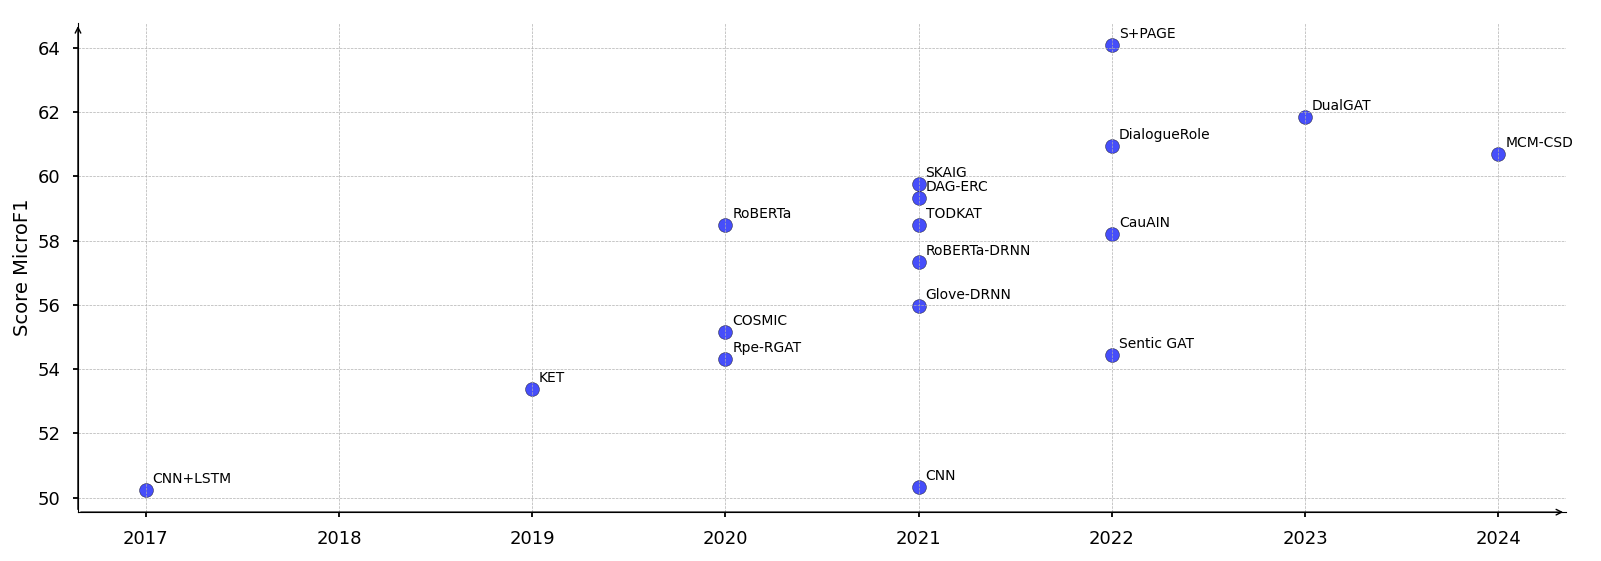
\includegraphics[width=0.9\textwidth]{sota-chrono-plot.png}
        \caption{\centering Modèles état-de-l'art en ERC suivant le microF1 sur les données textuelles de \texttt{DailyDialog} (6 étiquettes émotionnelles)}
    \end{figure}
    % \begin{figure}
    %     \centering
    %     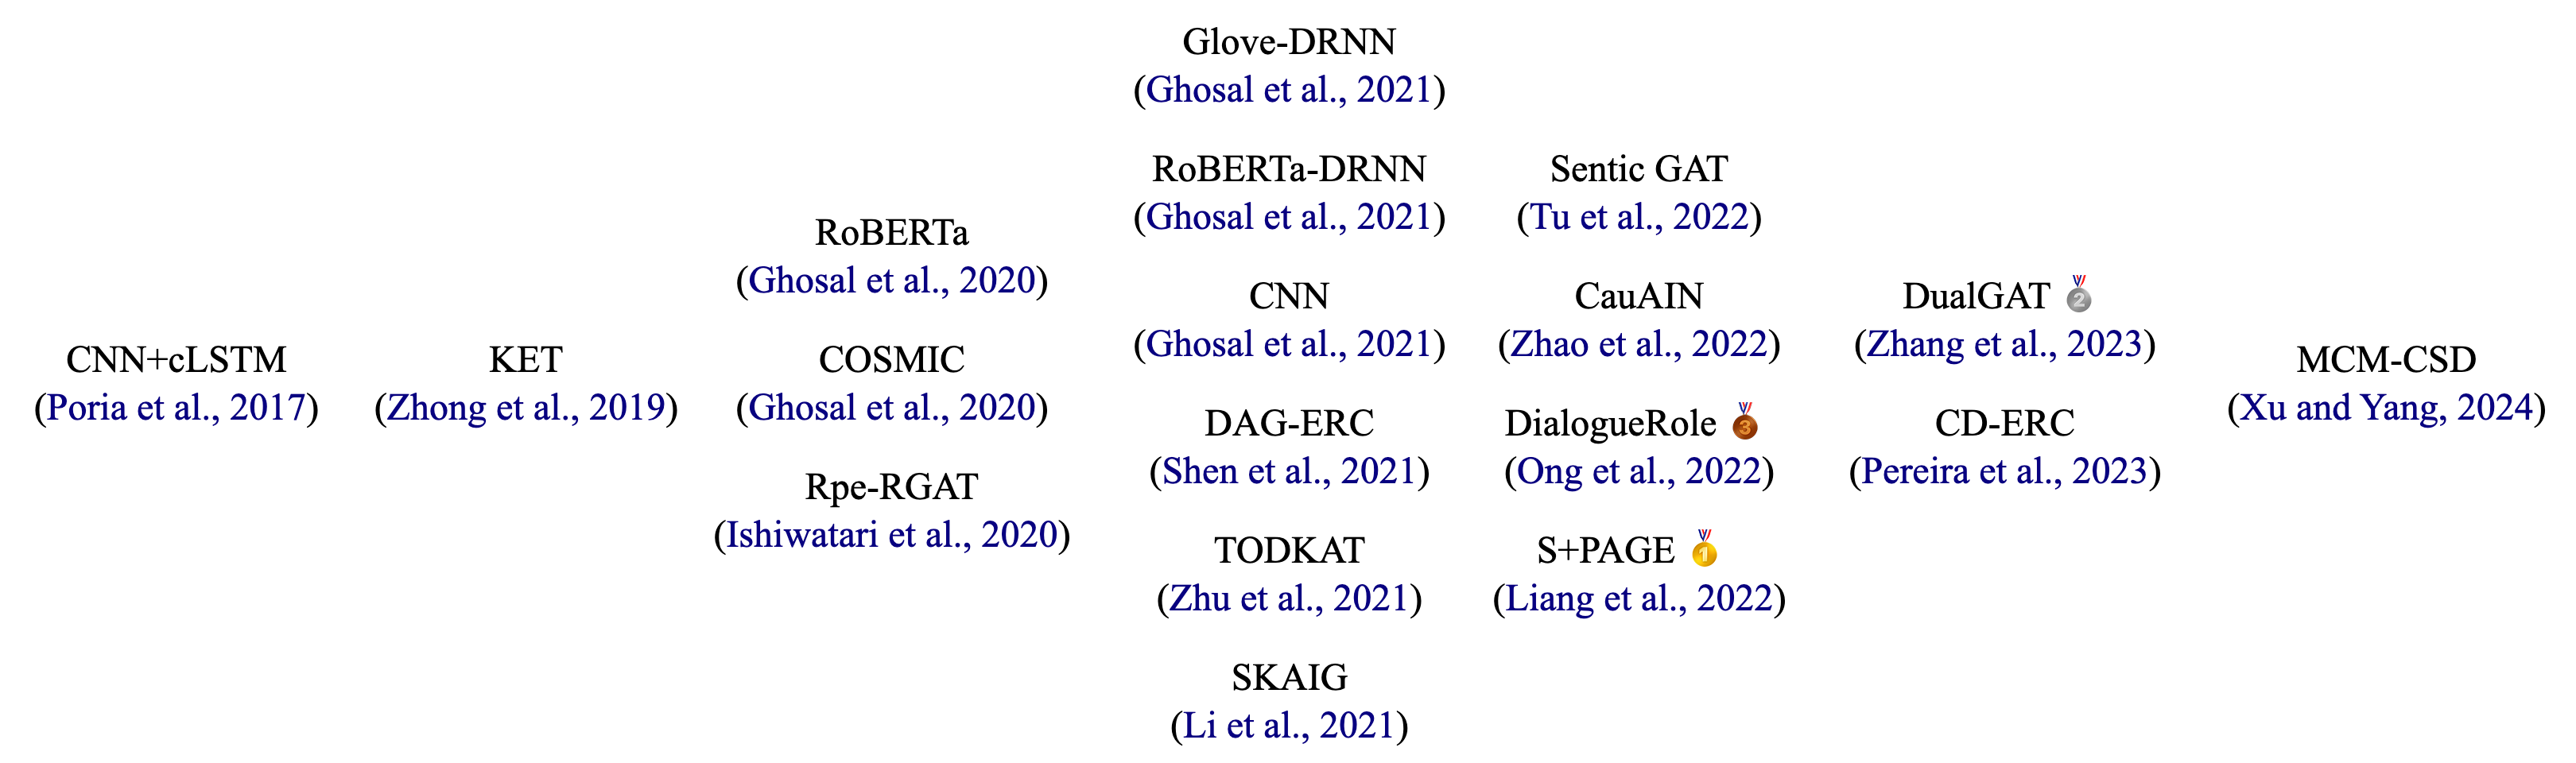
\includegraphics[width=\textwidth]{sota-chrono.png}
    %     \caption{\centering Modèles état-de-l'art en ERC. Les médailles indiquent les meilleurs scores microF1.}
    % \end{figure}
\end{frame}

\begin{frame}{Travaux connexes}
    % \emph{Ici un lien avec notre approche montrant la richesse de notre exploration des réseaux neuronaux. En effet, nous ne nous sommes pas limités aux derniers Transformers mais avons aussi testé des MLP, LSTM, Encoder-only et Decoder-only. Je pense que ça mérite d'être souligné.}
    \begin{figure}
        \centering
        \caption{\centering Vue d'ensemble des architectures de modèle utilisées par les modèles état-de-l'art en ERC. Les modèles \textbf{en gras} intègrent des graphes de connaissances.}
        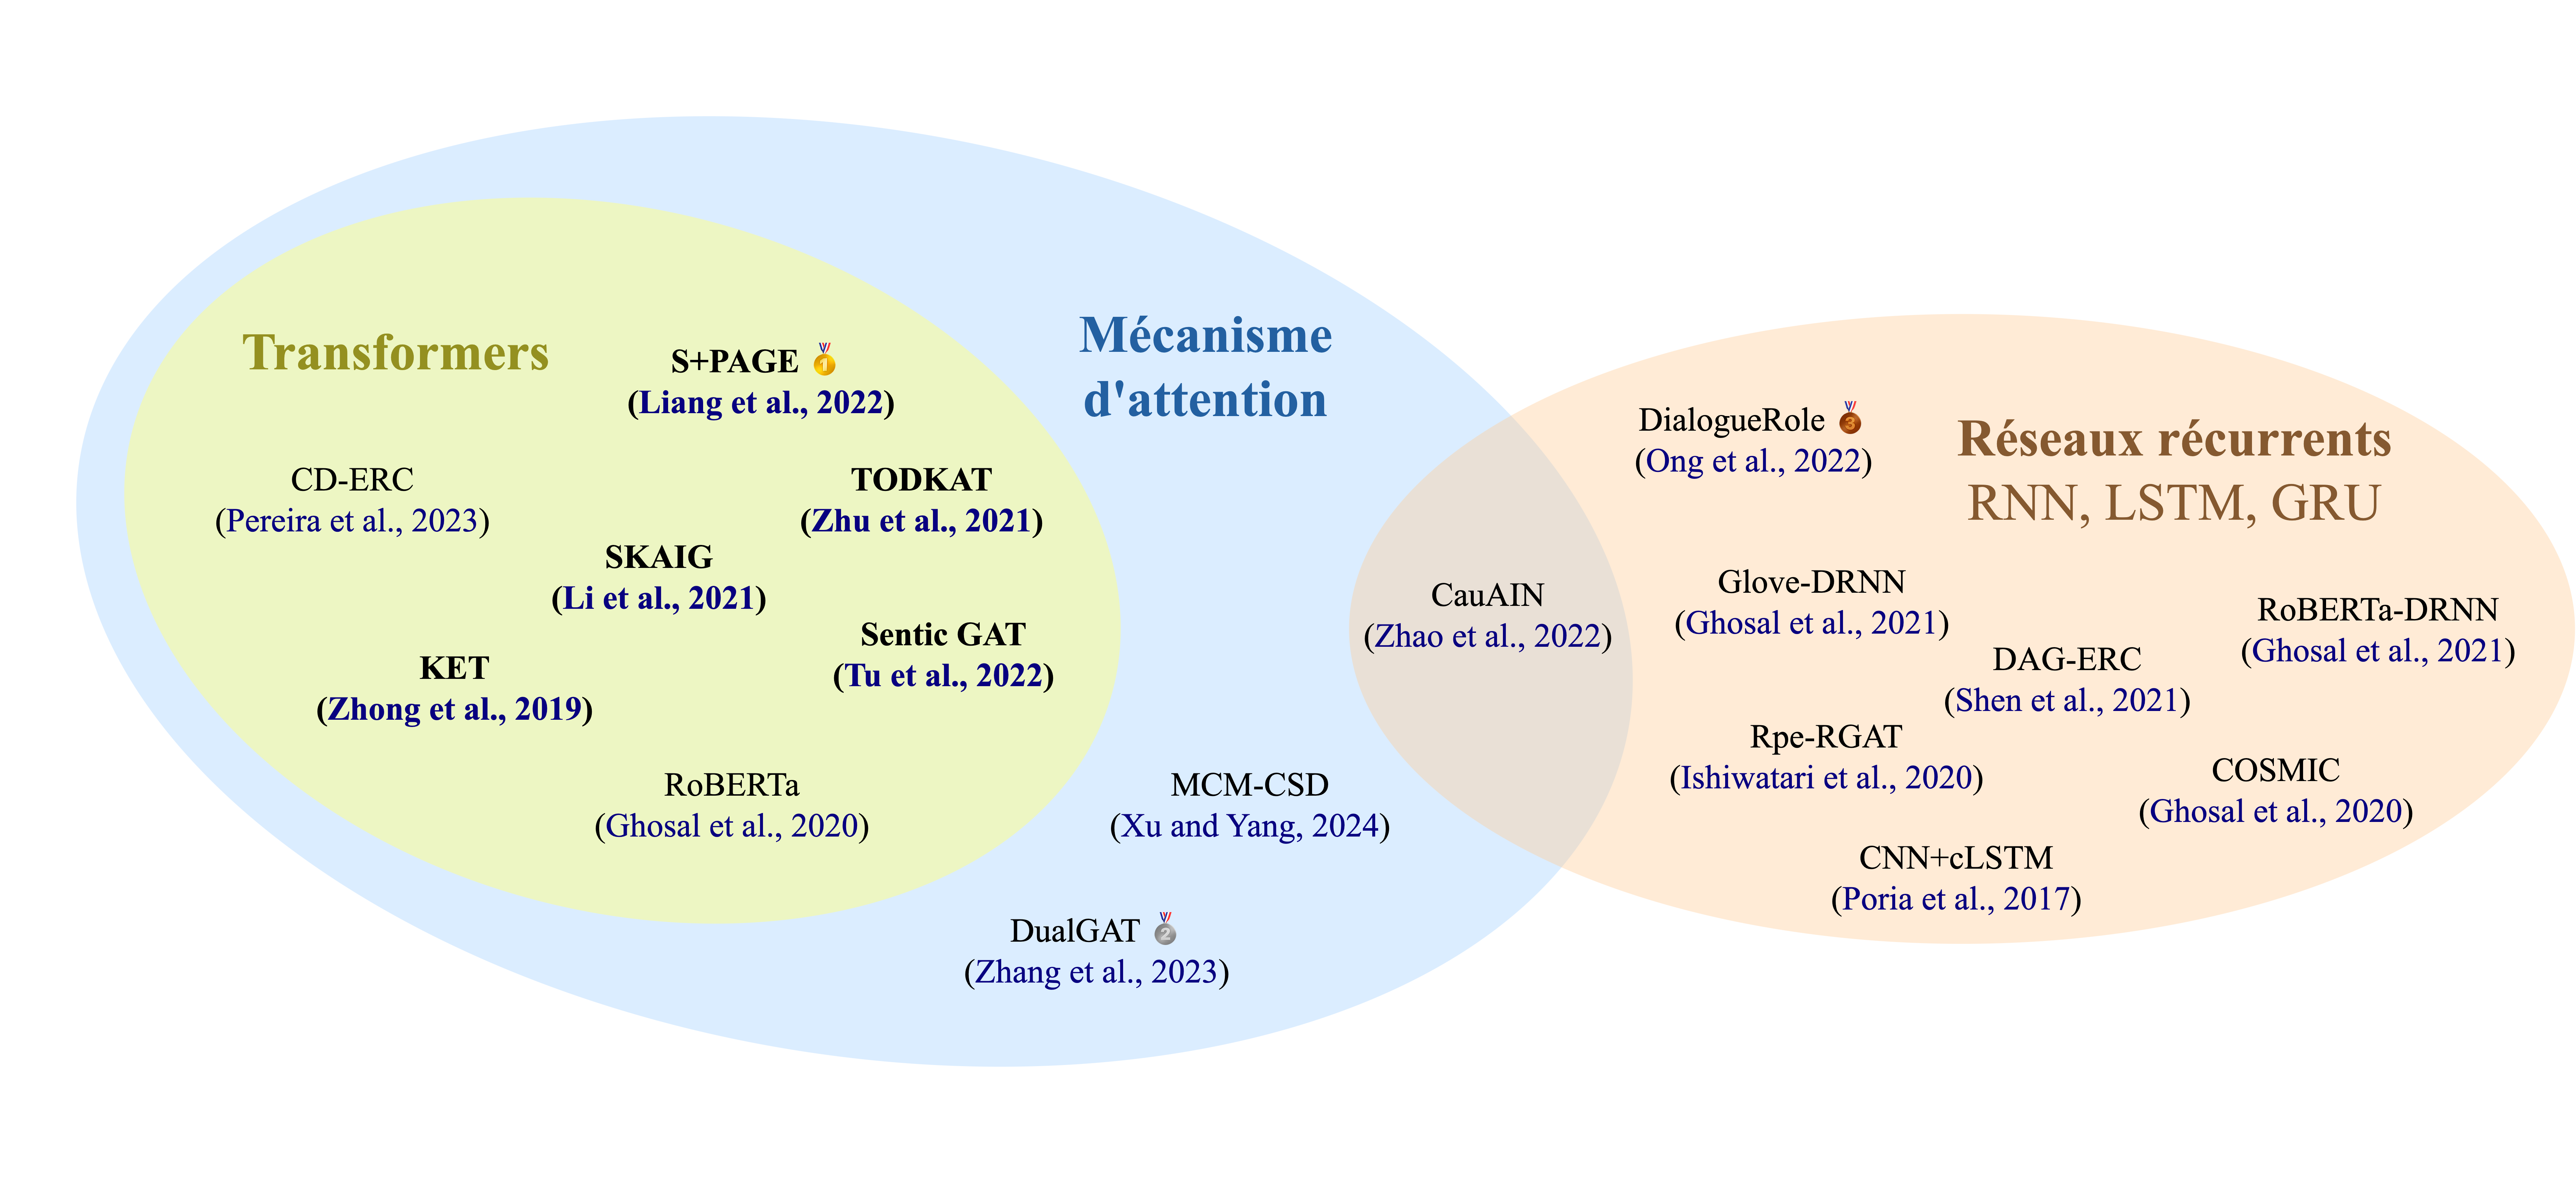
\includegraphics[width=0.9\textwidth]{sota-chrono-graph.png}
    \end{figure}
\end{frame}

\begin{frame}{Apports du \textsl{deep learning} et du \textsl{metric learning}}
    Les modèles neuronaux obtiennent des résultats état-de-l'art en ERC.~\manualcite{Poria et al., 2019, Pereira et al., 2022}\\
    %     \item Apprentissage sur le contexte grâce à l'\textcolor{roose}{\bf attention}~\footfullcite{Bahdanau:2014} et aux architectures associées~\footfullcite{Vaswani:2017}
    \vspace*{8pt}
    \visible<2->{
    Le \textsl{deep learning} par \textcolor{roose}{\bf apprentissage contrastif} permet :
    \begin{itemize}
        \item Un cadre de classification souple permettant l'extraction de relations entre les labels et la prédiction sur des labels inconnus%sans avoir besoin de changer le modèle ni l'entraînement
% L'extraction de relations entre les labels de manière assez naturelle puisque c'est comme ça que le modèle a été entraîné
        \item Une adaptation intrinsèque à l'apprentissage \textsl{few-shot} pour apprendre des émotions peu représentées
        \item Un variété d'architectures : réseaux de correspondances~\manualcite{Vinyals et al., 2016}, siamois~\manualcite{Koch et al., 2015}, prototypiques~\manualcite{Snell et al., 2017, Guibon et al., 2021}
    \end{itemize}
    }
\end{frame}

\begin{frame}{Réseaux siamois}
    \only<1>{
        \begin{figure}
            \centering
            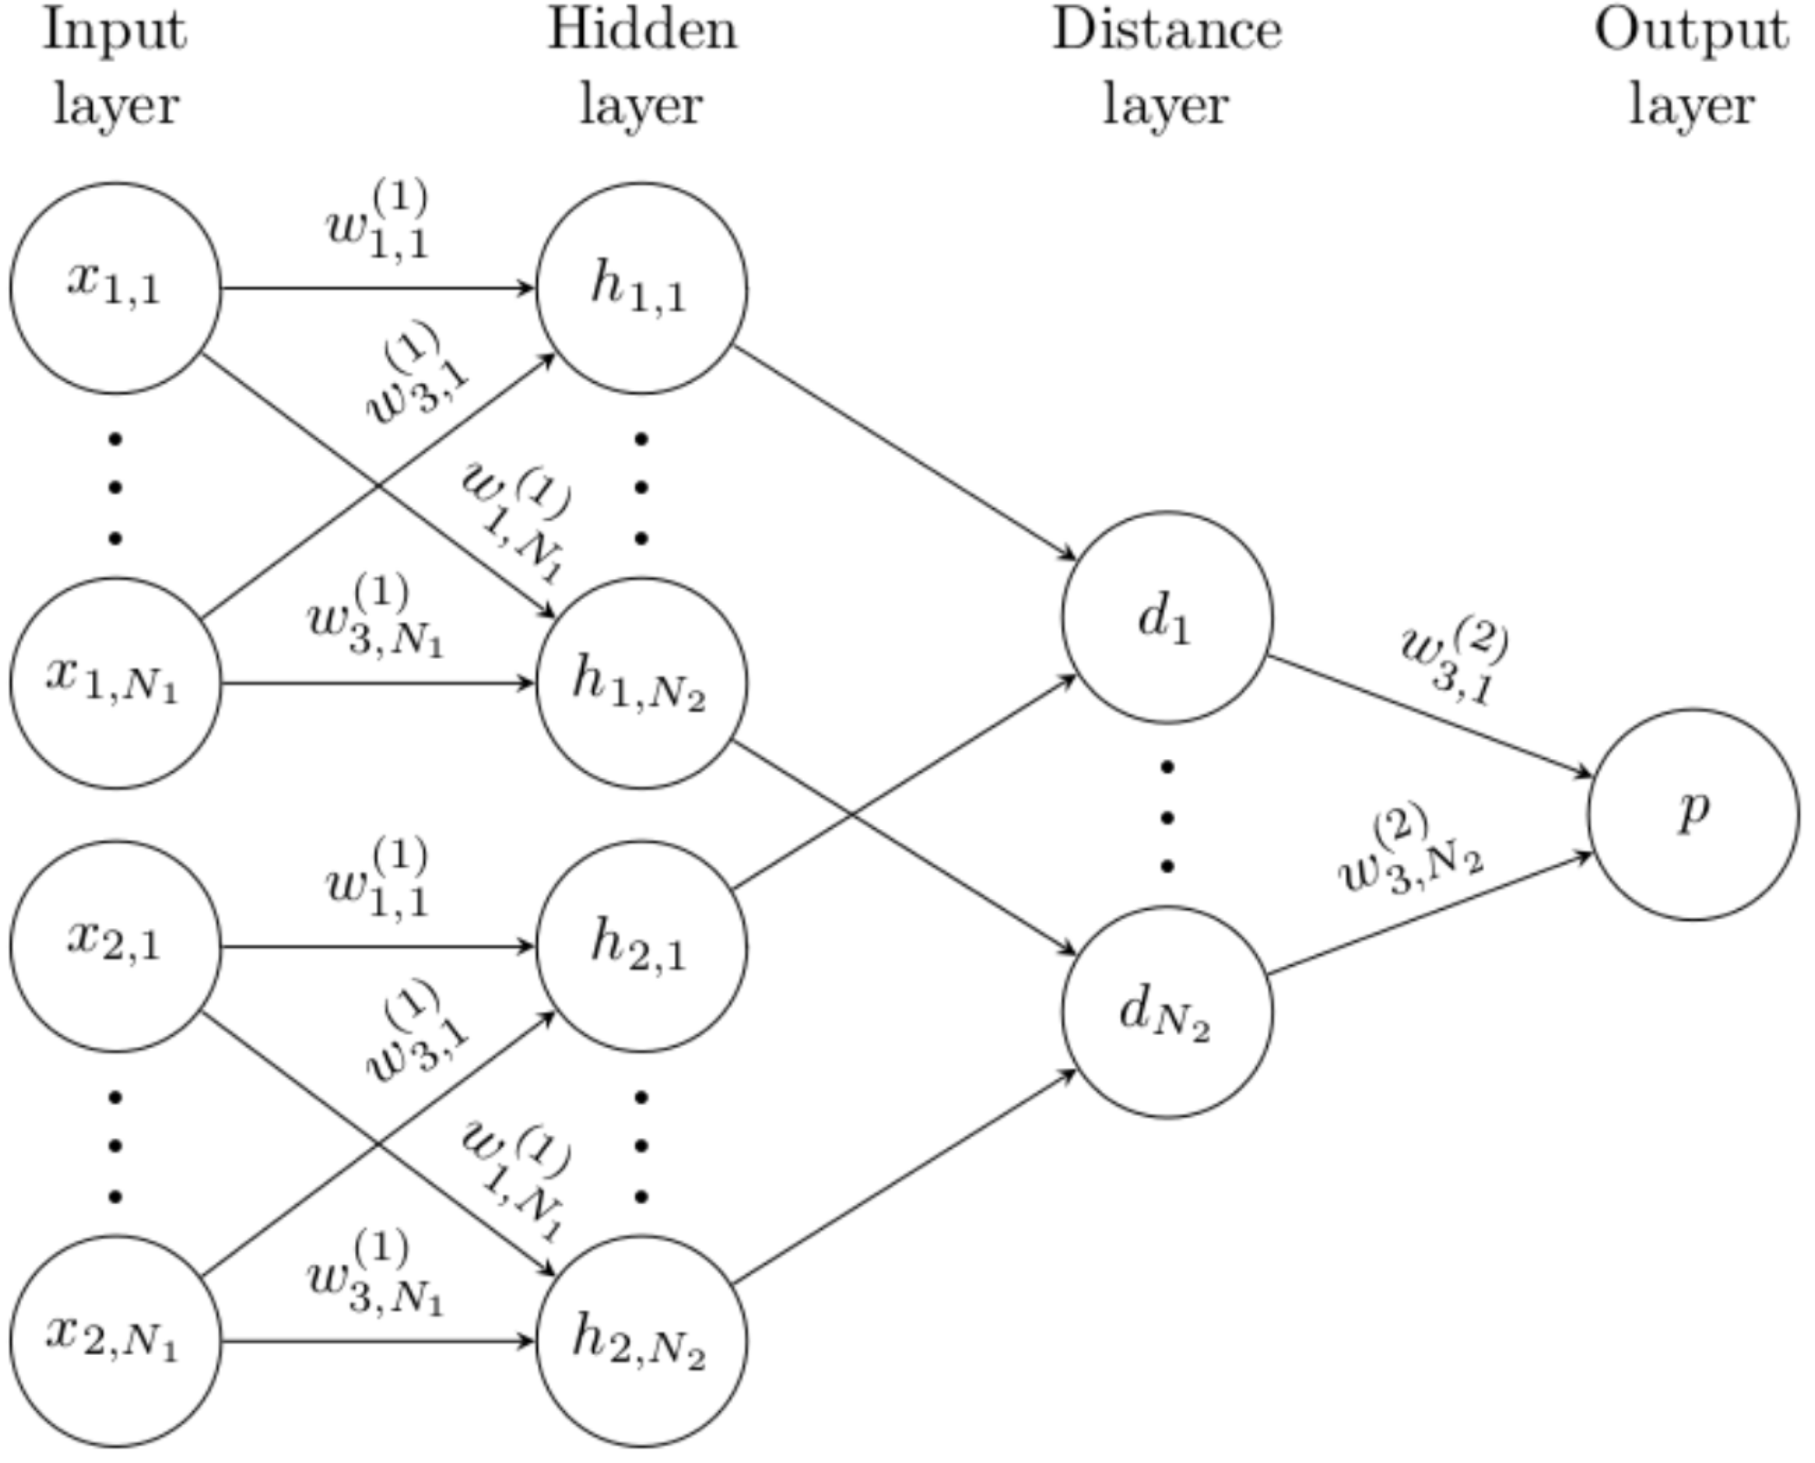
\includegraphics[width=0.52\textwidth]{koch1.png}
            \caption{\centering Architecture des réseaux siamois~\manualcite{Koch et al., 2015}}
        \end{figure}
    }
    \only<2>{
        \begin{figure}
            \centering
            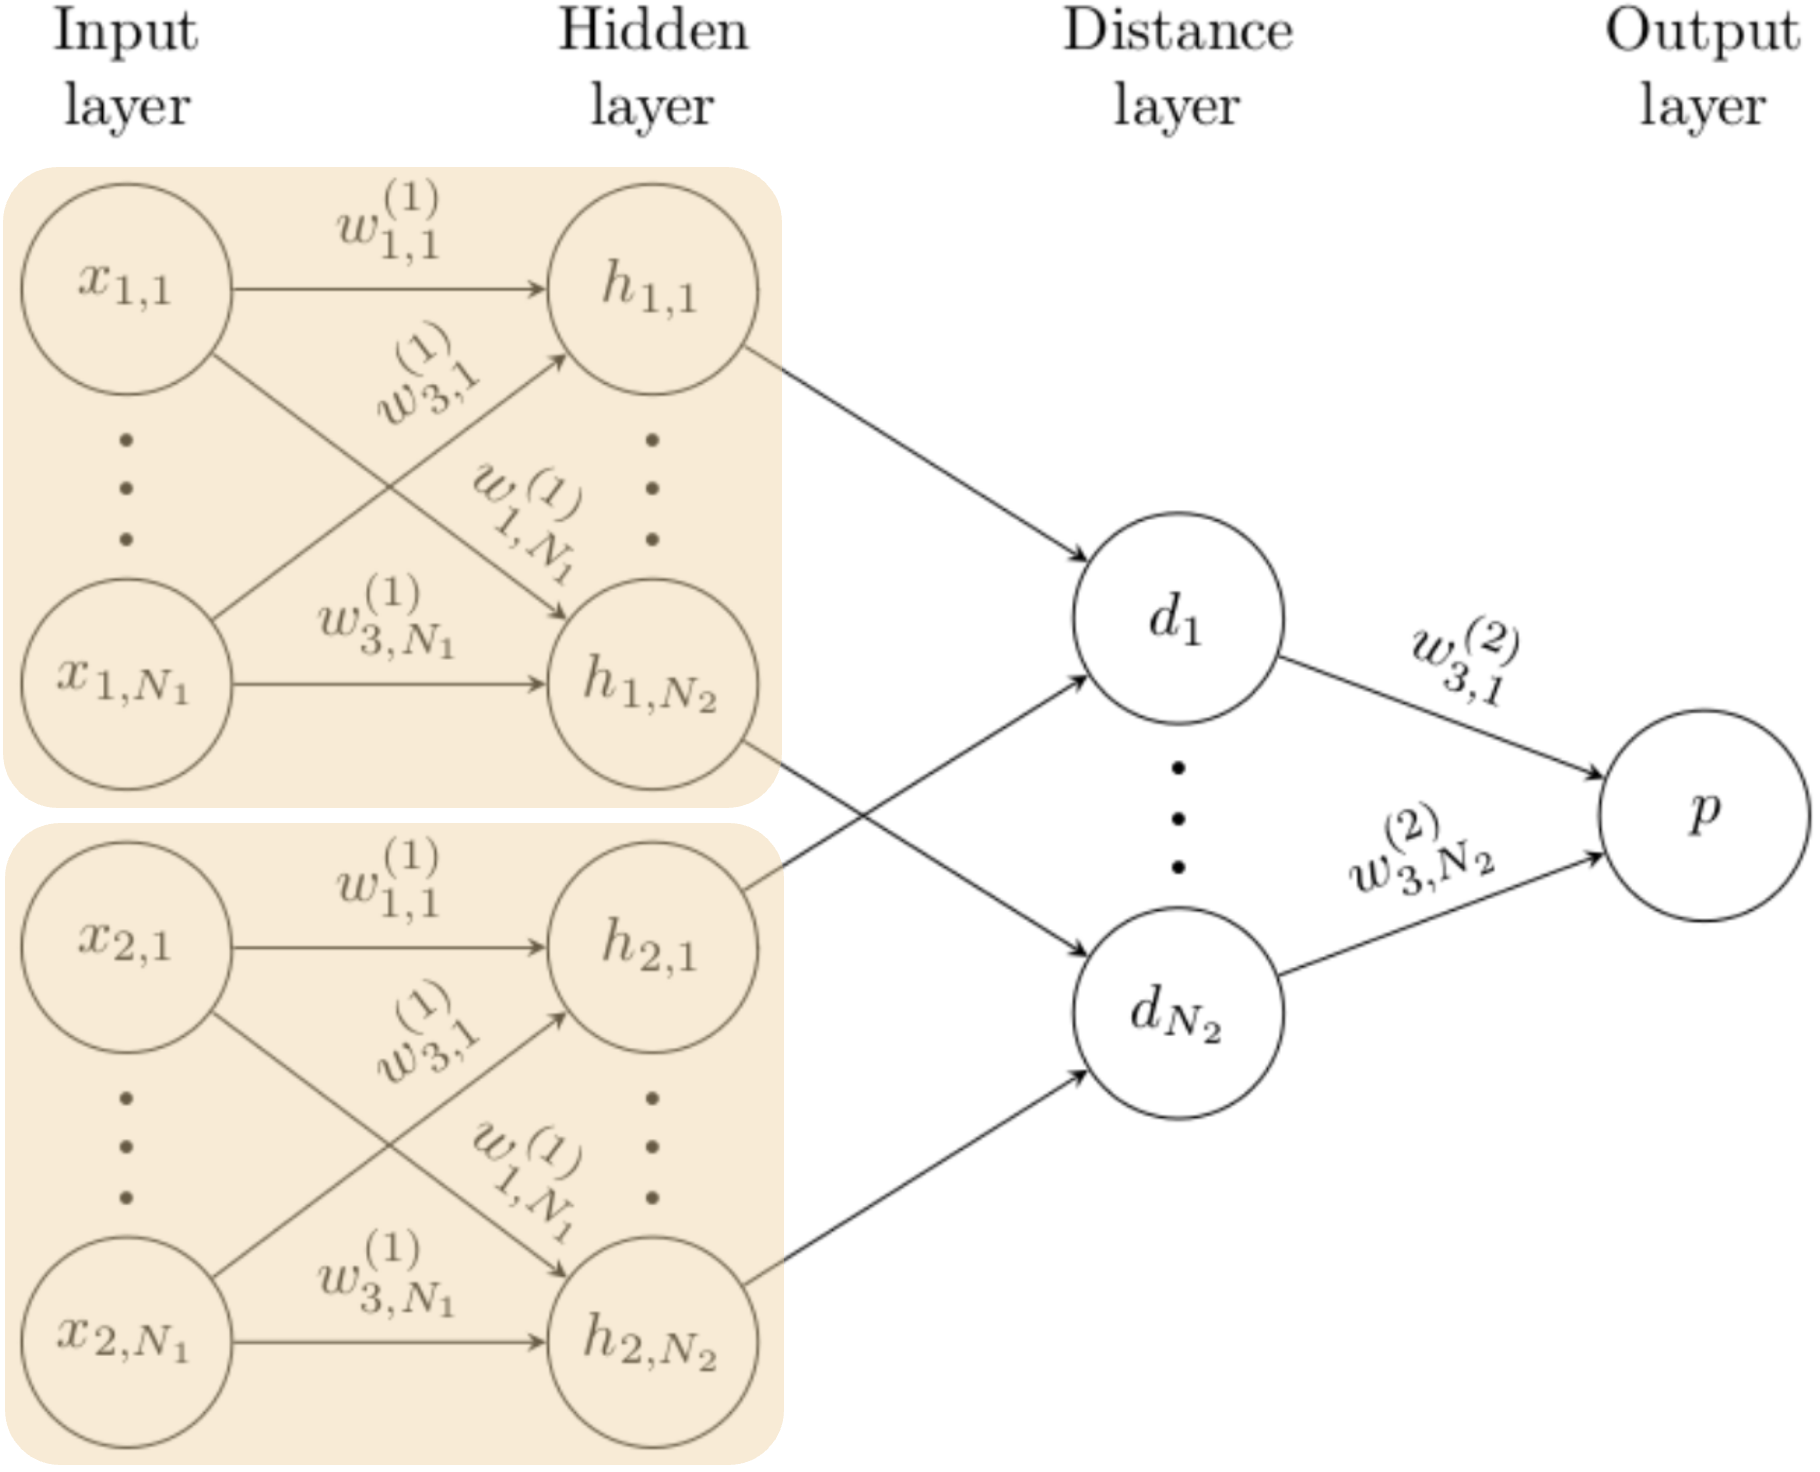
\includegraphics[width=0.52\textwidth]{koch2.png}
            \caption{\centering Architecture des réseaux siamois~\manualcite{Koch et al., 2015}}
        \end{figure}
    }
    \only<3>{
        \begin{figure}
            \centering
            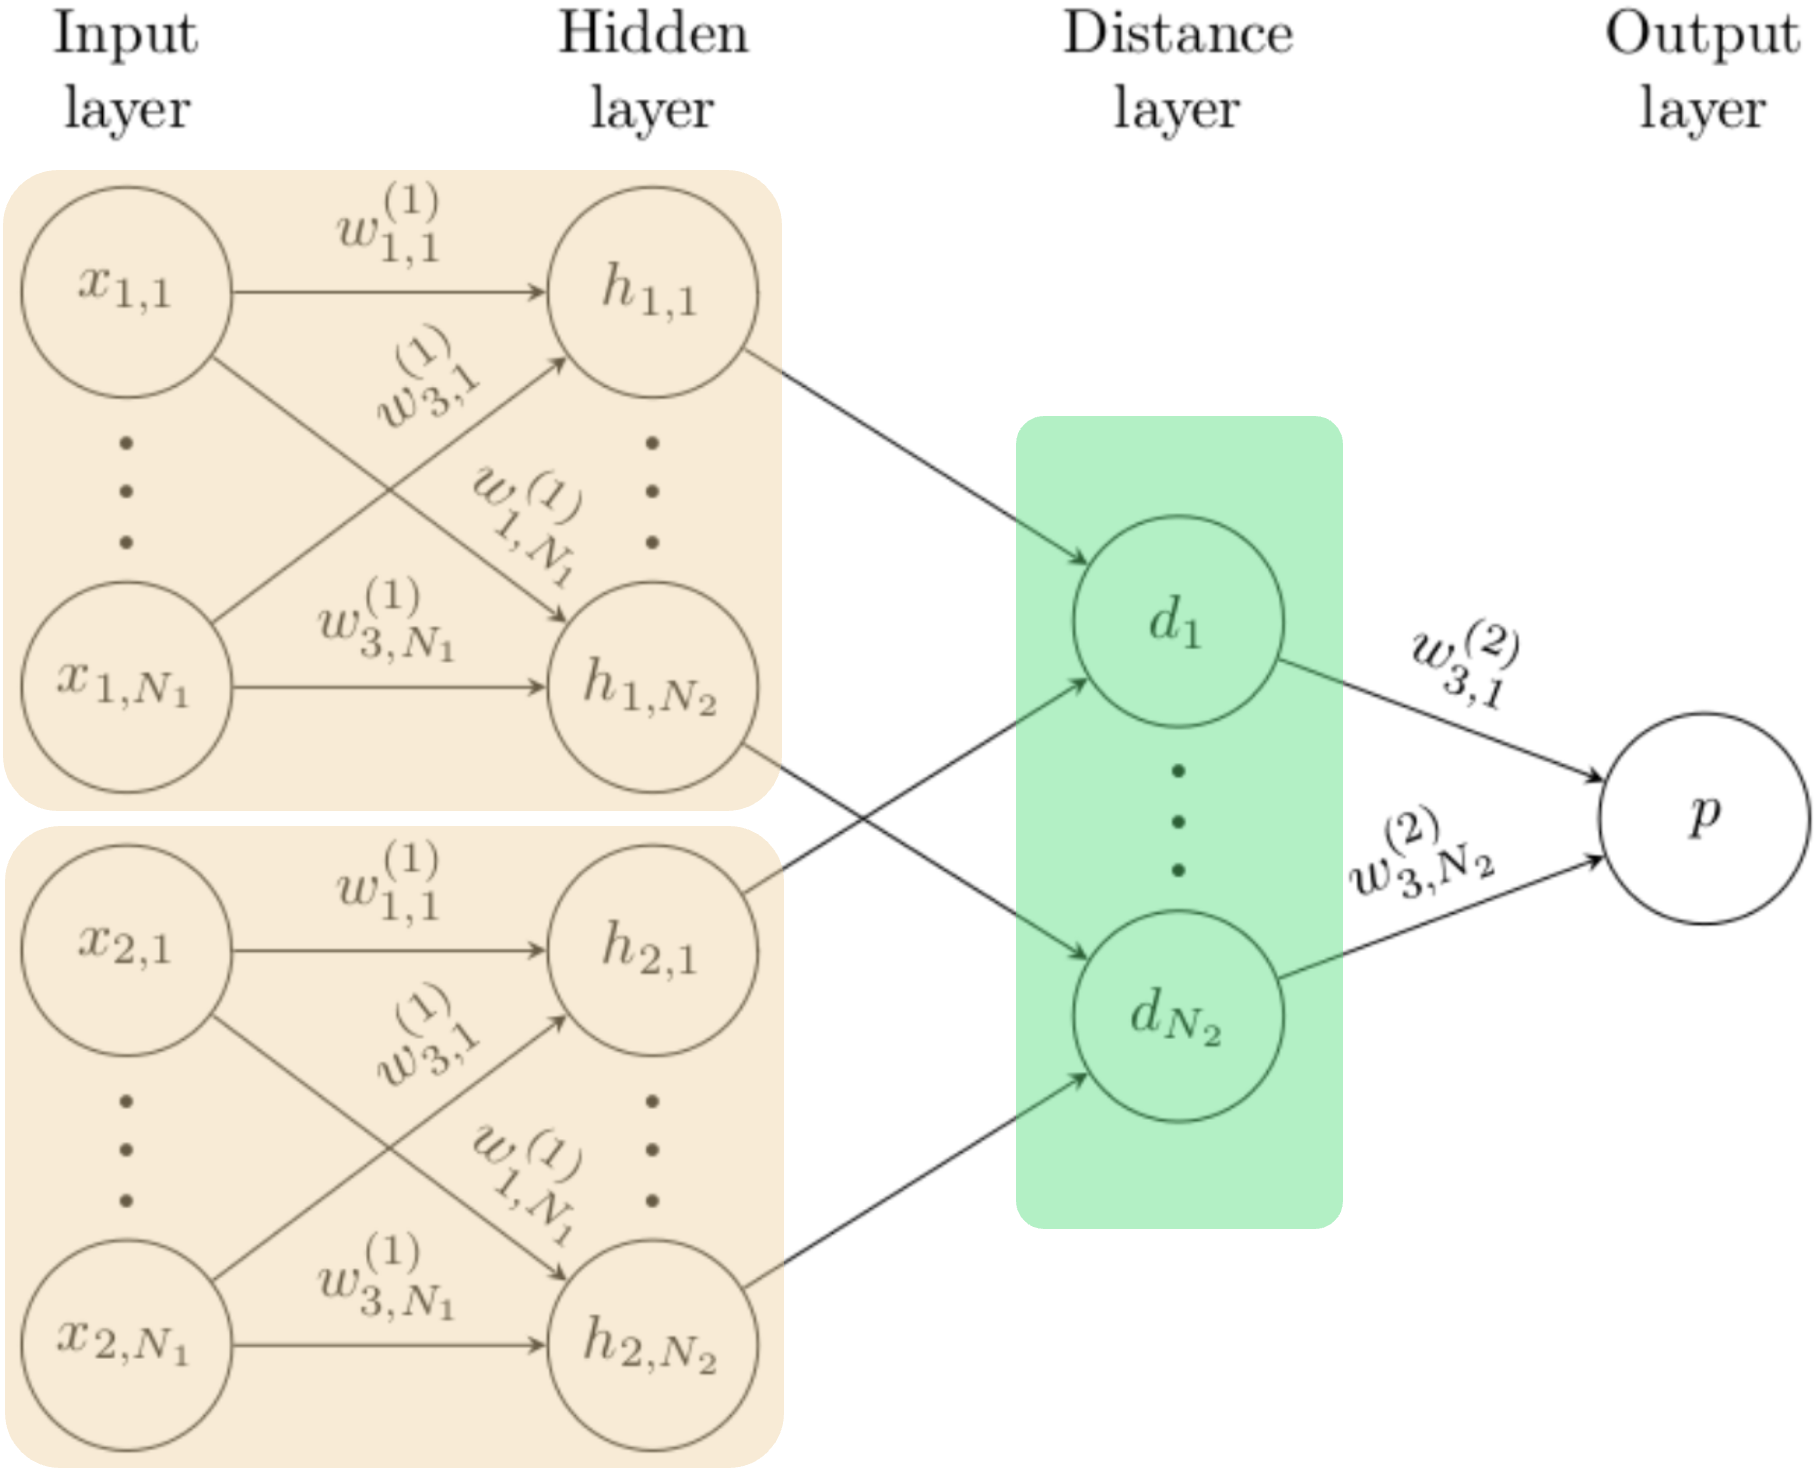
\includegraphics[width=0.52\textwidth]{koch3.png}
            \caption{\centering Architecture des réseaux siamois~\manualcite{Koch et al., 2015}}
        \end{figure}
    }
\end{frame}

\begin{frame}{\textsl{Triplet loss} : fonction de coût par triplets}

\begin{columns}
    \begin{column}{0.3\linewidth}
        Un triplet de propos:
            \begin{itemize}
                \item Ancre ($A$)
                \item Positif ($P$)
                \item Négatif ($N$)
            \end{itemize}
        \vspace{0.5cm}

        $A$ et $P$ sont de la même classe, $N$ est d'une autre.\\

        \vspace{0.5cm}
        Objectif de la \textsl{triplet loss}: 
        \begin{itemize}
        \item Minimiser \textcolor{roose}{$d(A,P)$}
        \item Maximiser \textcolor{roose}{$d(A,N)$}
        \end{itemize}
    \end{column}
    \begin{column}{0.65\linewidth}
\visible<2->{
        \begin{equation*}
            \mathcal{L}(a, p, n) = \text{max}\left\{ \textcolor<3>{roose}{d(a, p) - d(a, n)} + \textcolor<4>{blue}{\texttt{marge}}, 0\right\}
        \end{equation*}
        
        \only<2-3>{
            \begin{figure}
                \centering
                
\includegraphics[width=0.8\textwidth]{triplet_loss_no_margin.png}
                \caption{\centering Illustration du principe de la \textsl{triplet loss}}
            \end{figure}
        }
        \only<4>{
            \begin{figure}
                \centering
                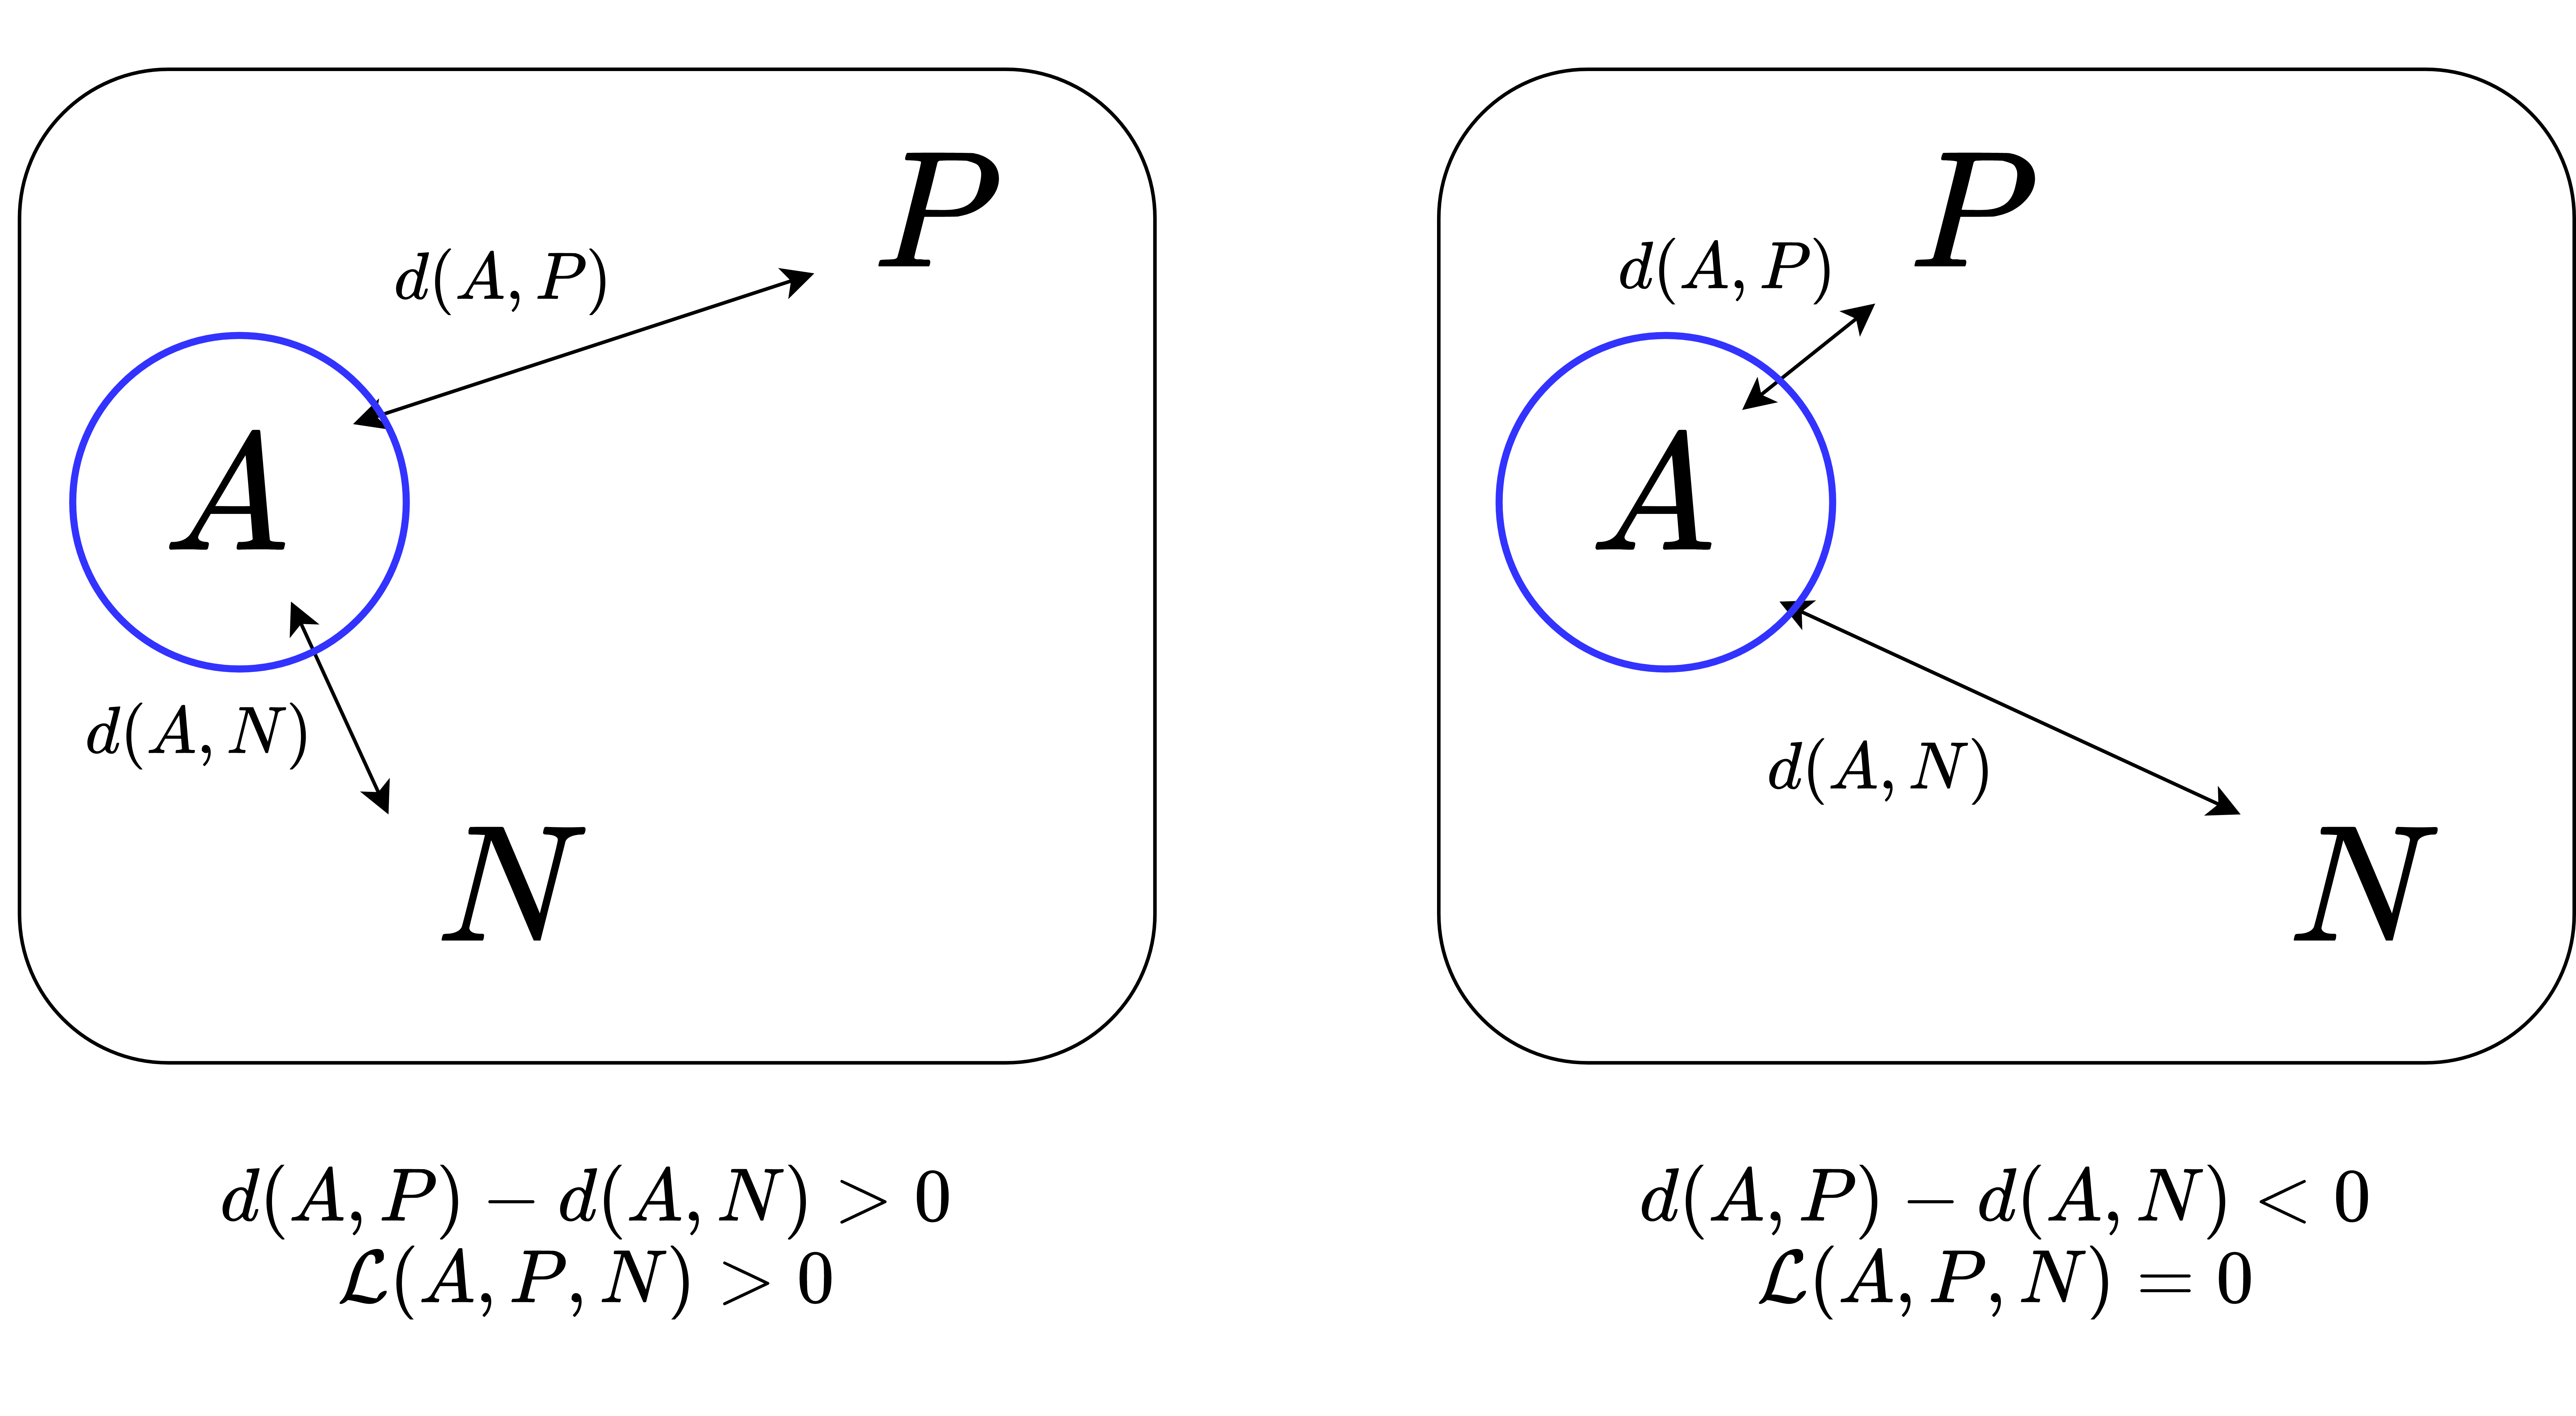
\includegraphics[width=0.8\textwidth]{triplet_loss_margin.png}
                \caption{\centering Illustration du principe de la \textsl{triplet loss}}
            \end{figure}
        }
}
    \end{column}
\end{columns}

\end{frame}

\section{Méthodologie}

\begin{frame}{Données}
    Jeu de données \texttt{DailyDialog}~\manualcite{Li et al., 2017}
    \begin{itemize}
        \item 13 118 dialogues dyadiques en anglais sur des sujets de la vie quotidienne
        \item Annotation \textcolor{roose}{\bf au niveau du tour de parole} : \texttt{happiness}, \texttt{anger}, \texttt{disgust}, \texttt{fear}, \texttt{surprise}, \texttt{sadness} et \texttt{no emotion}
    \end{itemize}
\vspace*{5pt}
\visible<2->{
    \begin{figure}[h]
        \centering
        % \caption{\centering Description des données de \texttt{DailyDialog}}
        \begin{subfigure}[t]{0.45\textwidth}
            \centering
            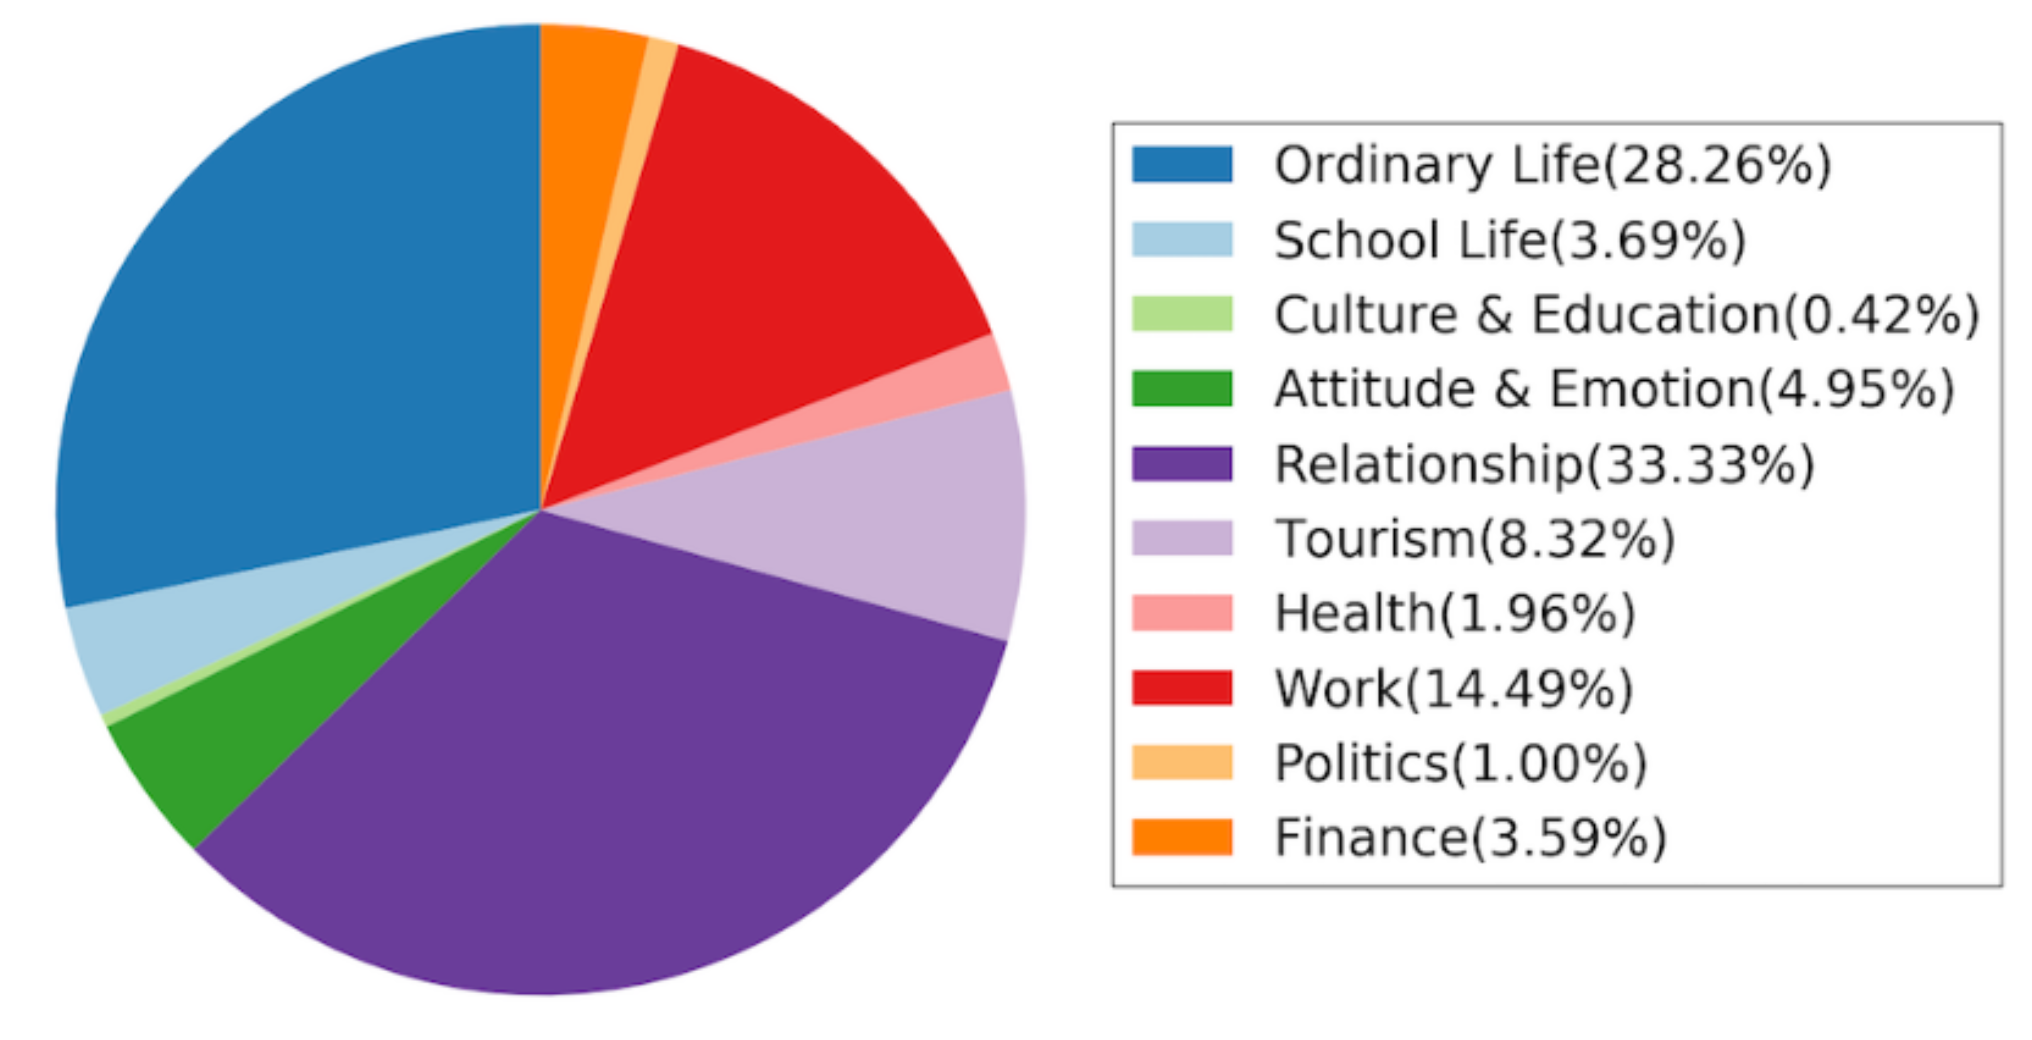
\includegraphics[width=\textwidth]{topic-distib.png}
            \caption{\centering Répartition des sujets des dialogues}
            \label{fig:topics}
        \end{subfigure}
        \hfill
        \begin{subfigure}[t]{0.45\textwidth}
            \centering
            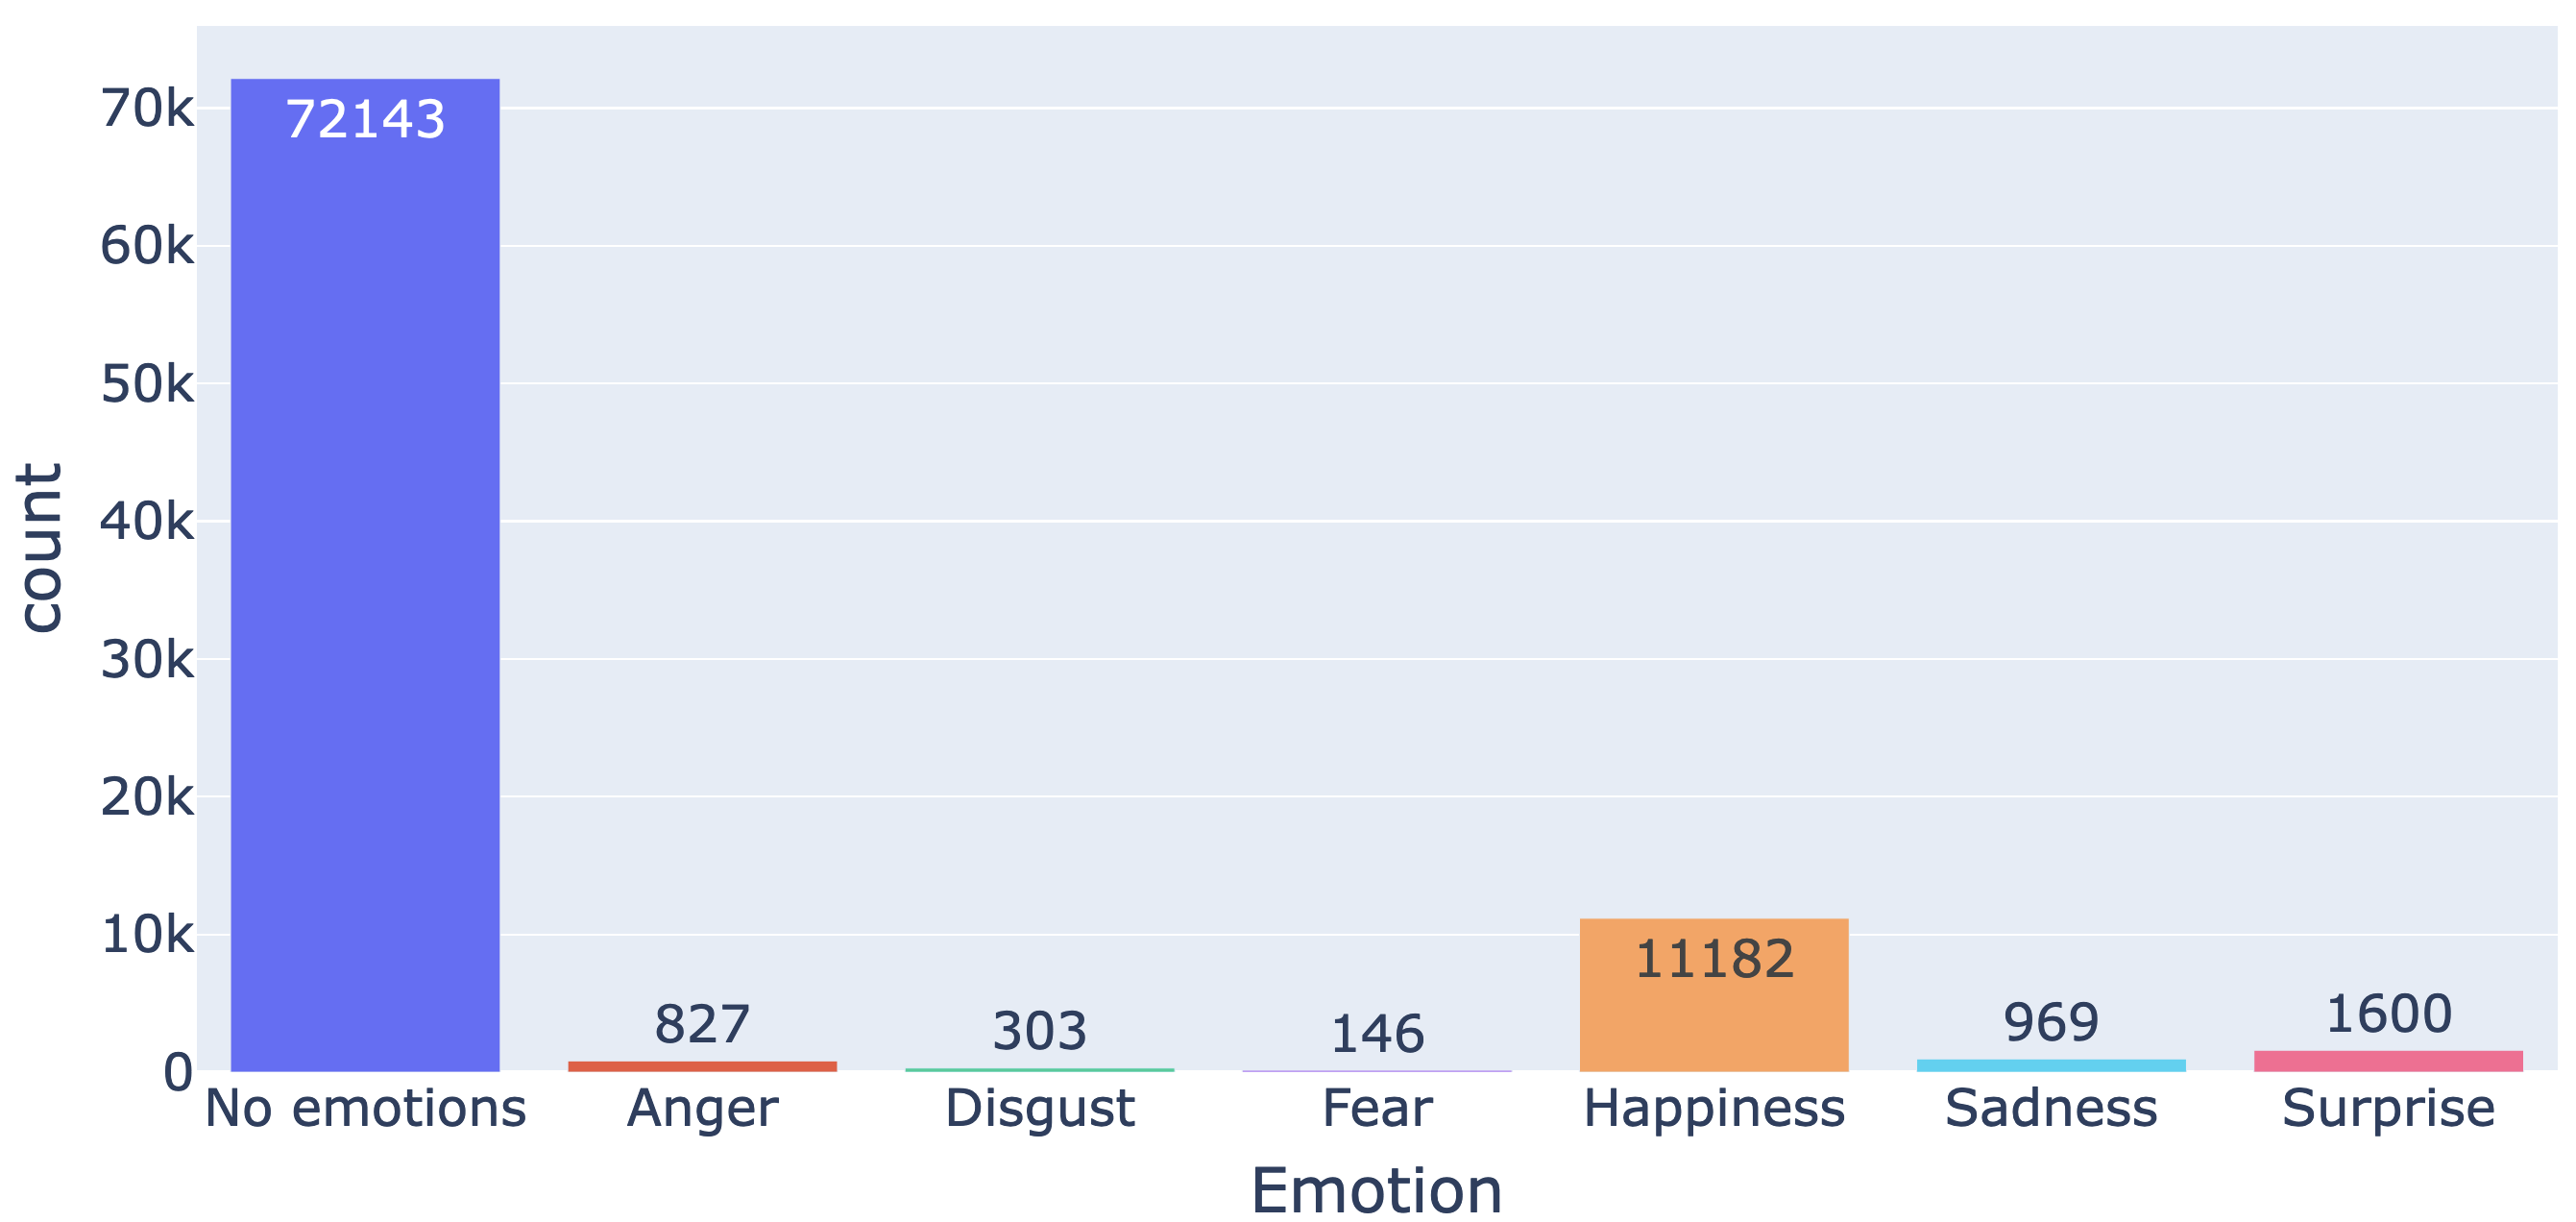
\includegraphics[width=\textwidth]{train-pretty.png}
            \caption{\centering Distribution des émotions dans les données d'entraînement}
            \label{fig:emotions}
        \end{subfigure}
        \label{fig:dd-desc}
    \end{figure}
}
\end{frame}

\begin{frame}{Procédure d'entraînement - prédictions d'émotions avec contexte}
    \begin{figure}
        \centering
        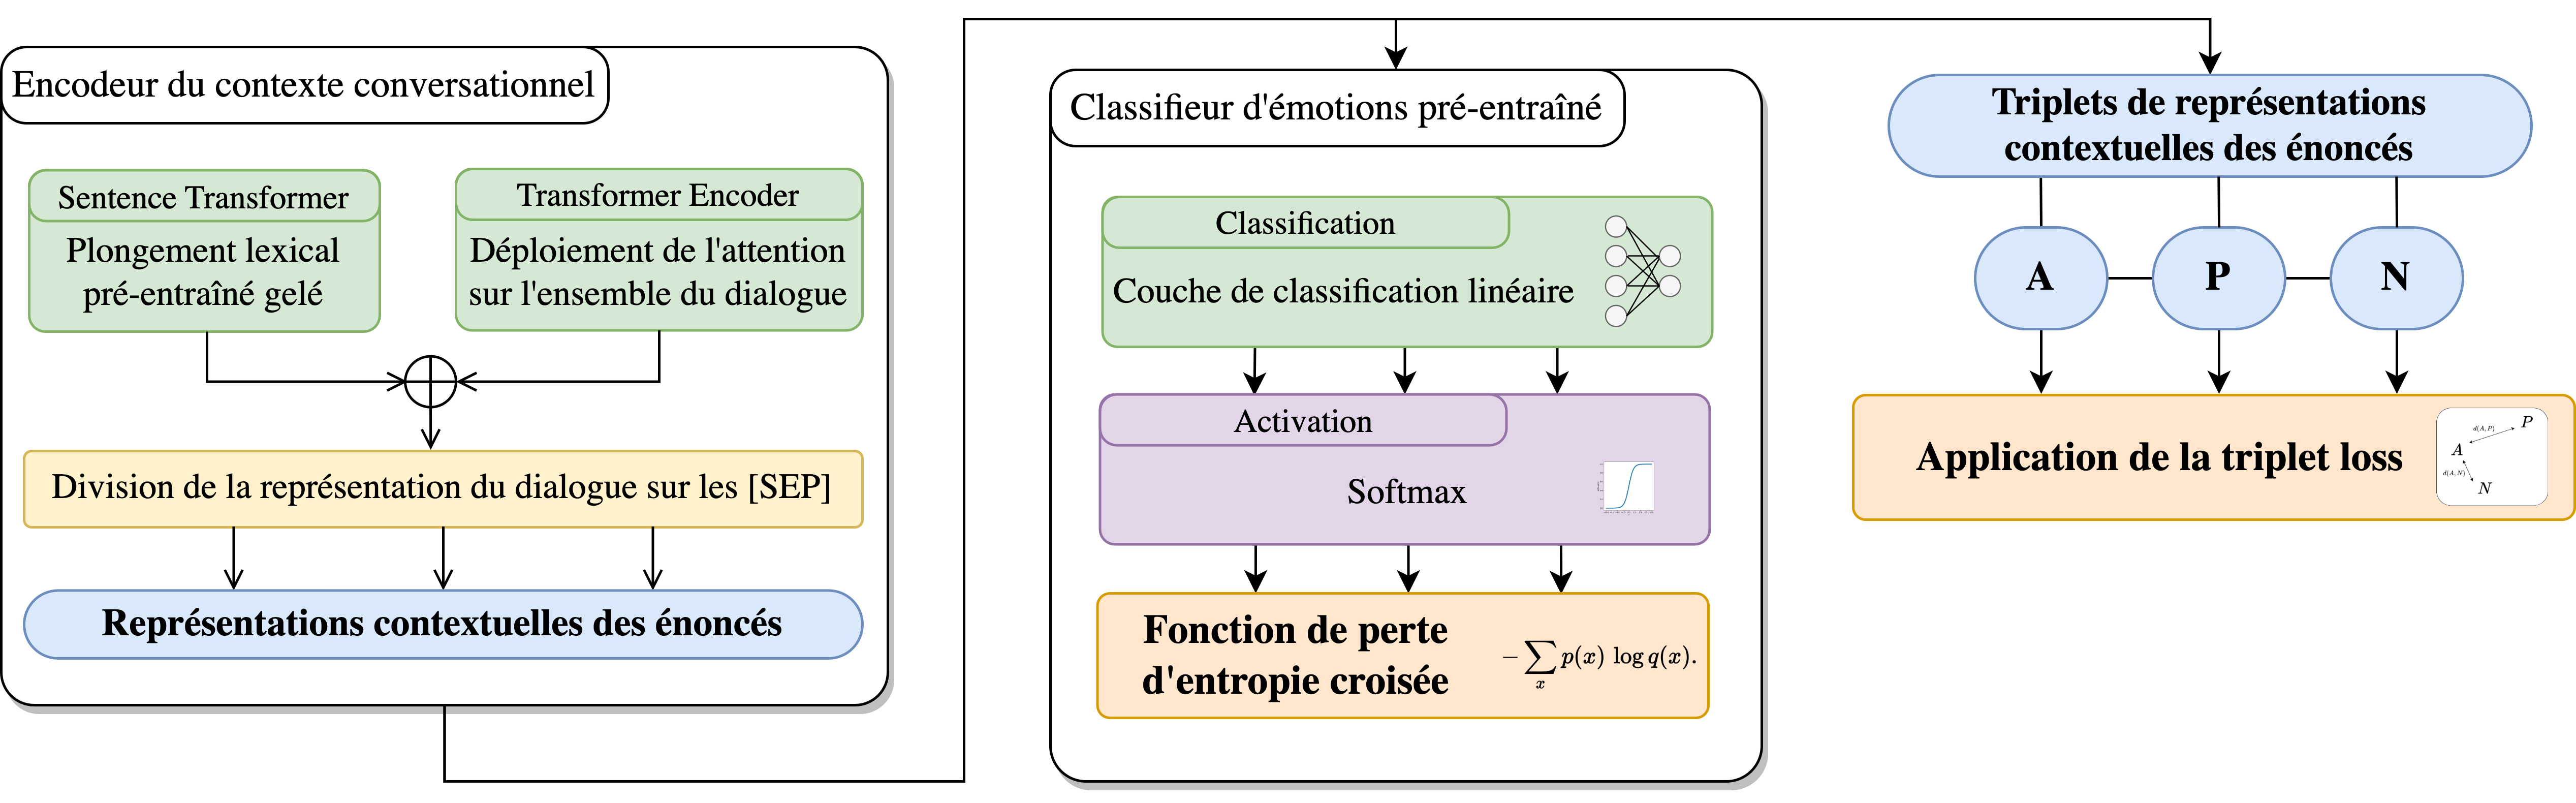
\includegraphics[width=\textwidth]{contextual_utterances_training_fr.png}
        \caption{\centering Prédiction d'émotions sur des représentations de propos contextuelles.}
    \end{figure}
\end{frame}

\begin{frame}{Métriques d'évaluation}
\begin{itemize}
    \item MicroF1 : choix historiquement privilégié par la littérature
    \item MacroF1 : métrique plus exigeante qui favorise une \textcolor{roose}{\bf reconnaissance émotionnelle polyvalente}
    \item MCC (\textsl{Matthews Correlation Coefficient}) : métrique plus contraignante utilisée pour des classes fortement déséquilibrées
\end{itemize}
\visible<2->{
Le MCC est défini comme suit~\manualcite{Matthews, 1975} :
\begin{equation}
    \text{MCC} = \frac{\mathit{TP}/ N-S \times P}{\sqrt{P S(1-S)(1-P)}}
\end{equation}
Où $TP$ est le nombre de vrais positifs, $N$ la taille des données, $P$ la précision et $S$ le rappel (pour \textsl{sensitivity}).
}
\end{frame}

\section{Résultats}

\begin{frame}{Résultats quantitatifs}
    % Préciser que c'est sur le jeu de test d'origine, et que l'astérisque signifie qu'on exclut l'étiquette neutre
    \begin{minipage}{0.6\textwidth}
        \centering
        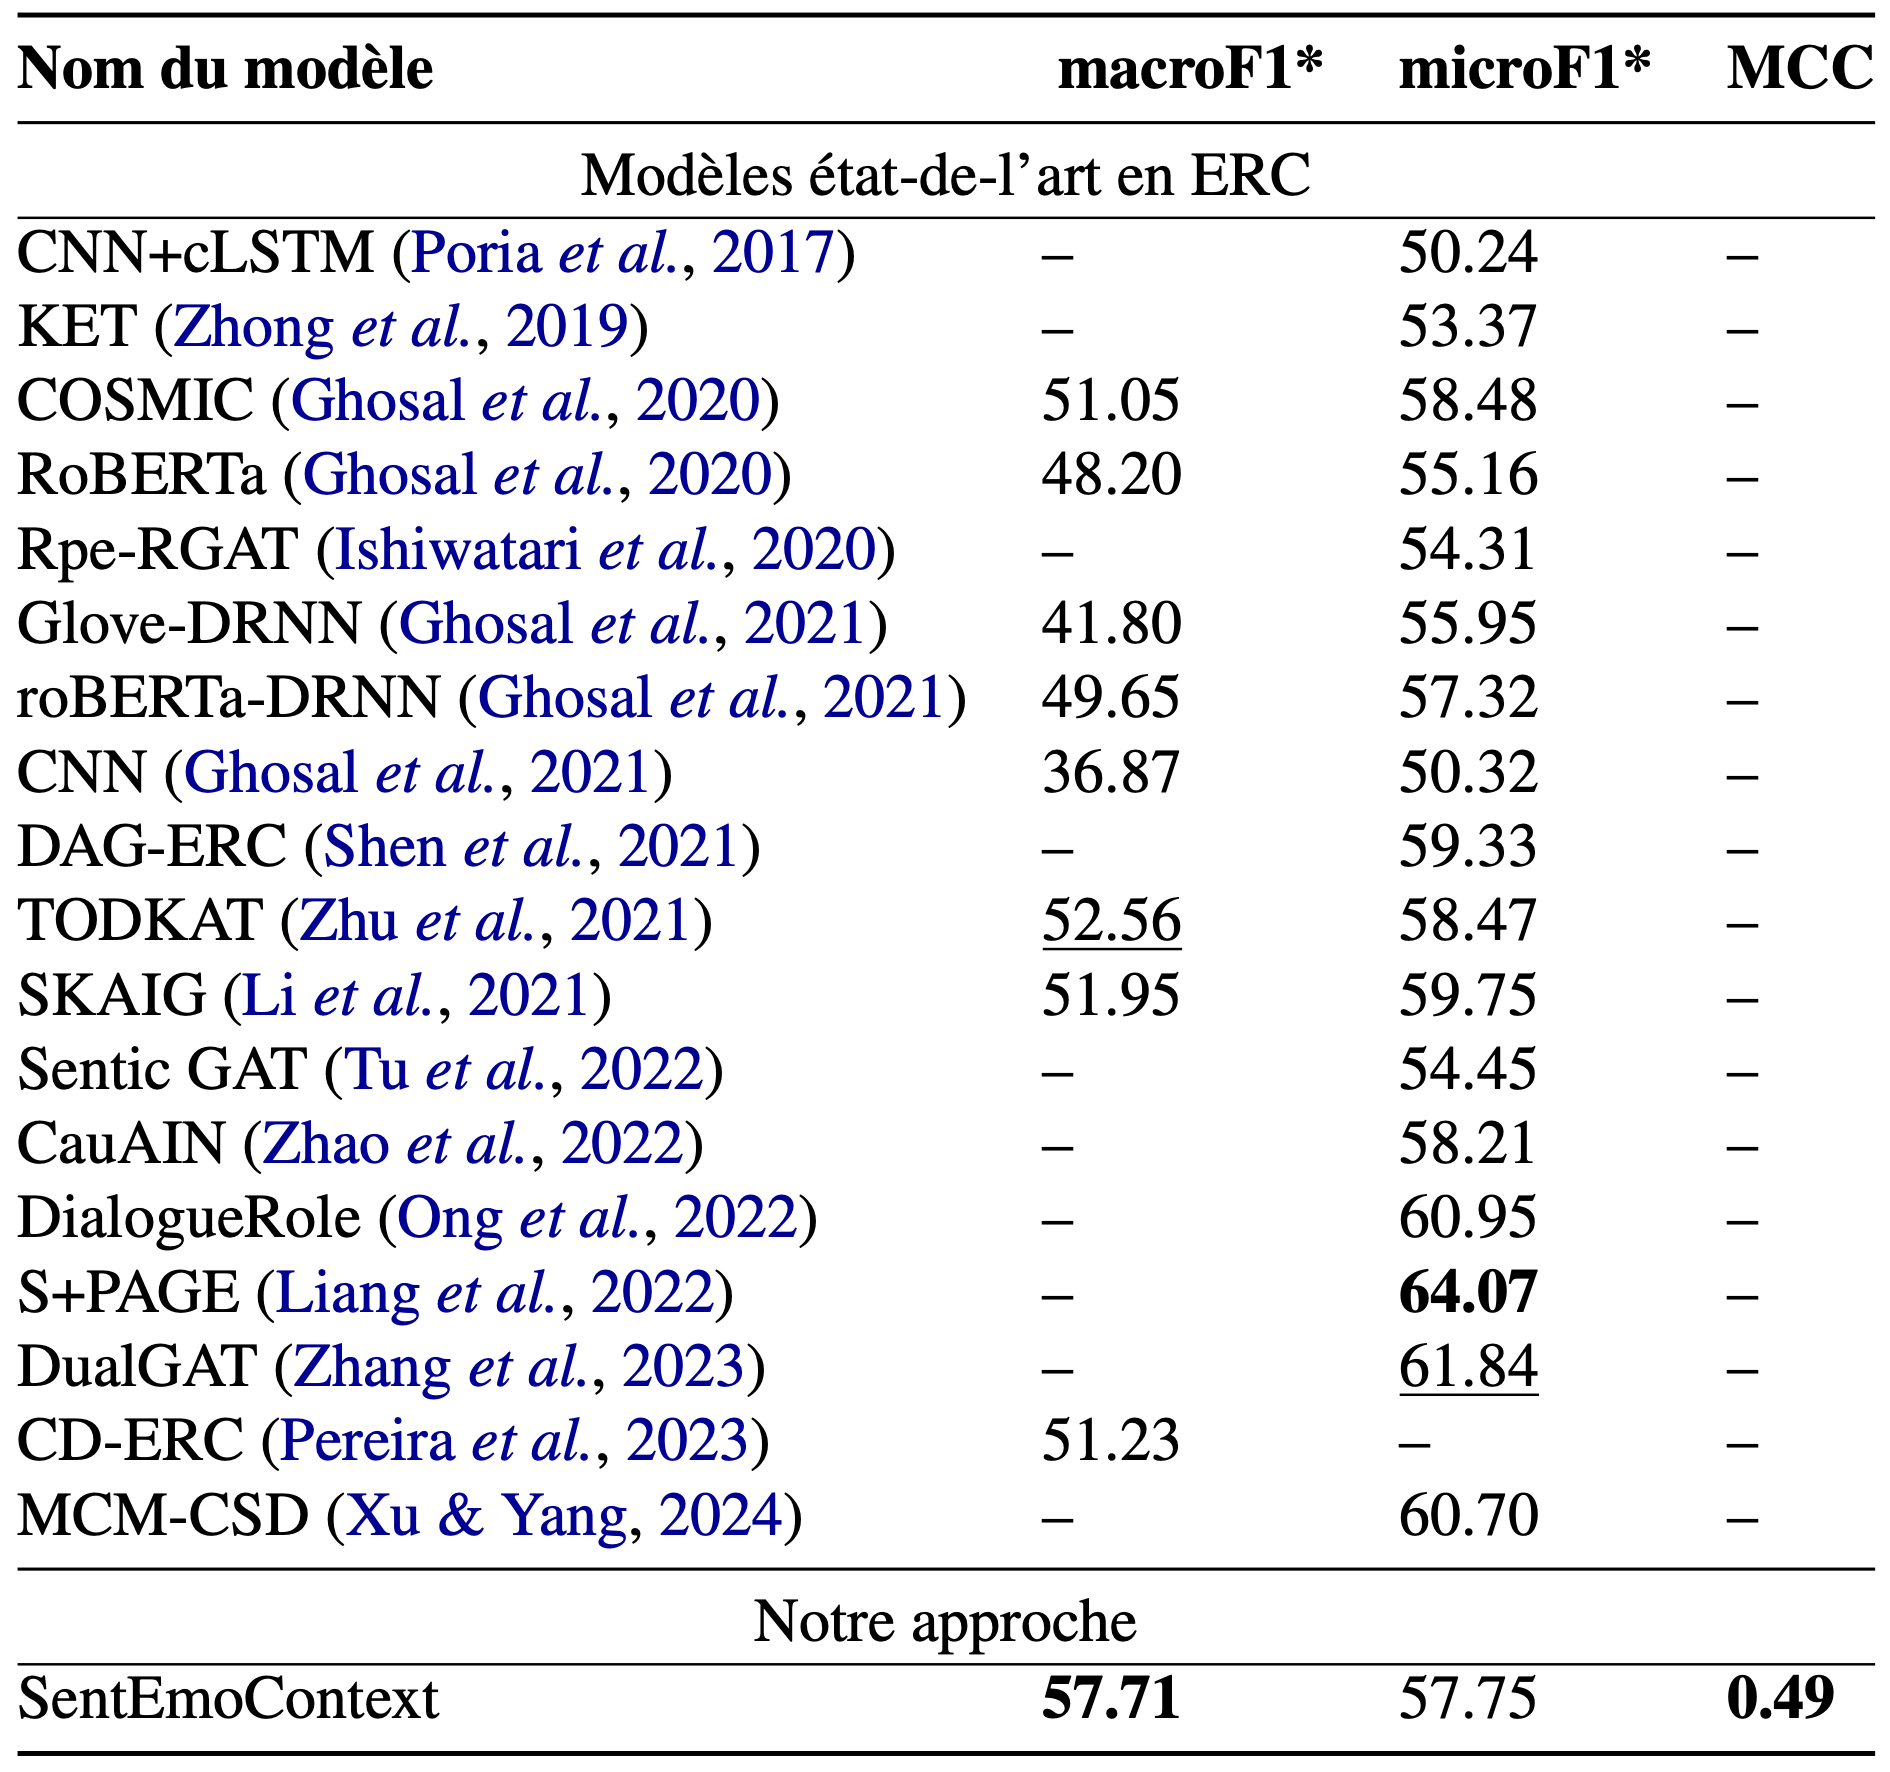
\includegraphics[scale=0.23]{results-2024.png}
    \end{minipage}%
    \begin{minipage}{0.4\textwidth}
        \centering
        \captionof{figure}{Résultats en ERC sur \texttt{DailyDialog}}
    \end{minipage}
\end{frame}

\begin{frame}{Évaluation qualitative}
    \begin{itemize}
        \item Impact de l'information contextuelle
    \end{itemize}
    % Montre à quel point il est difficile de tirer partie positivement du contexte conversationnel. Si on a des éxemples ou le contexte peut aider (CDH), il y en a aussi ou le contexte est vecteur d'une information importante qui ne semble pas réussir à se transferer
    \begin{figure}[h]
        \centering
        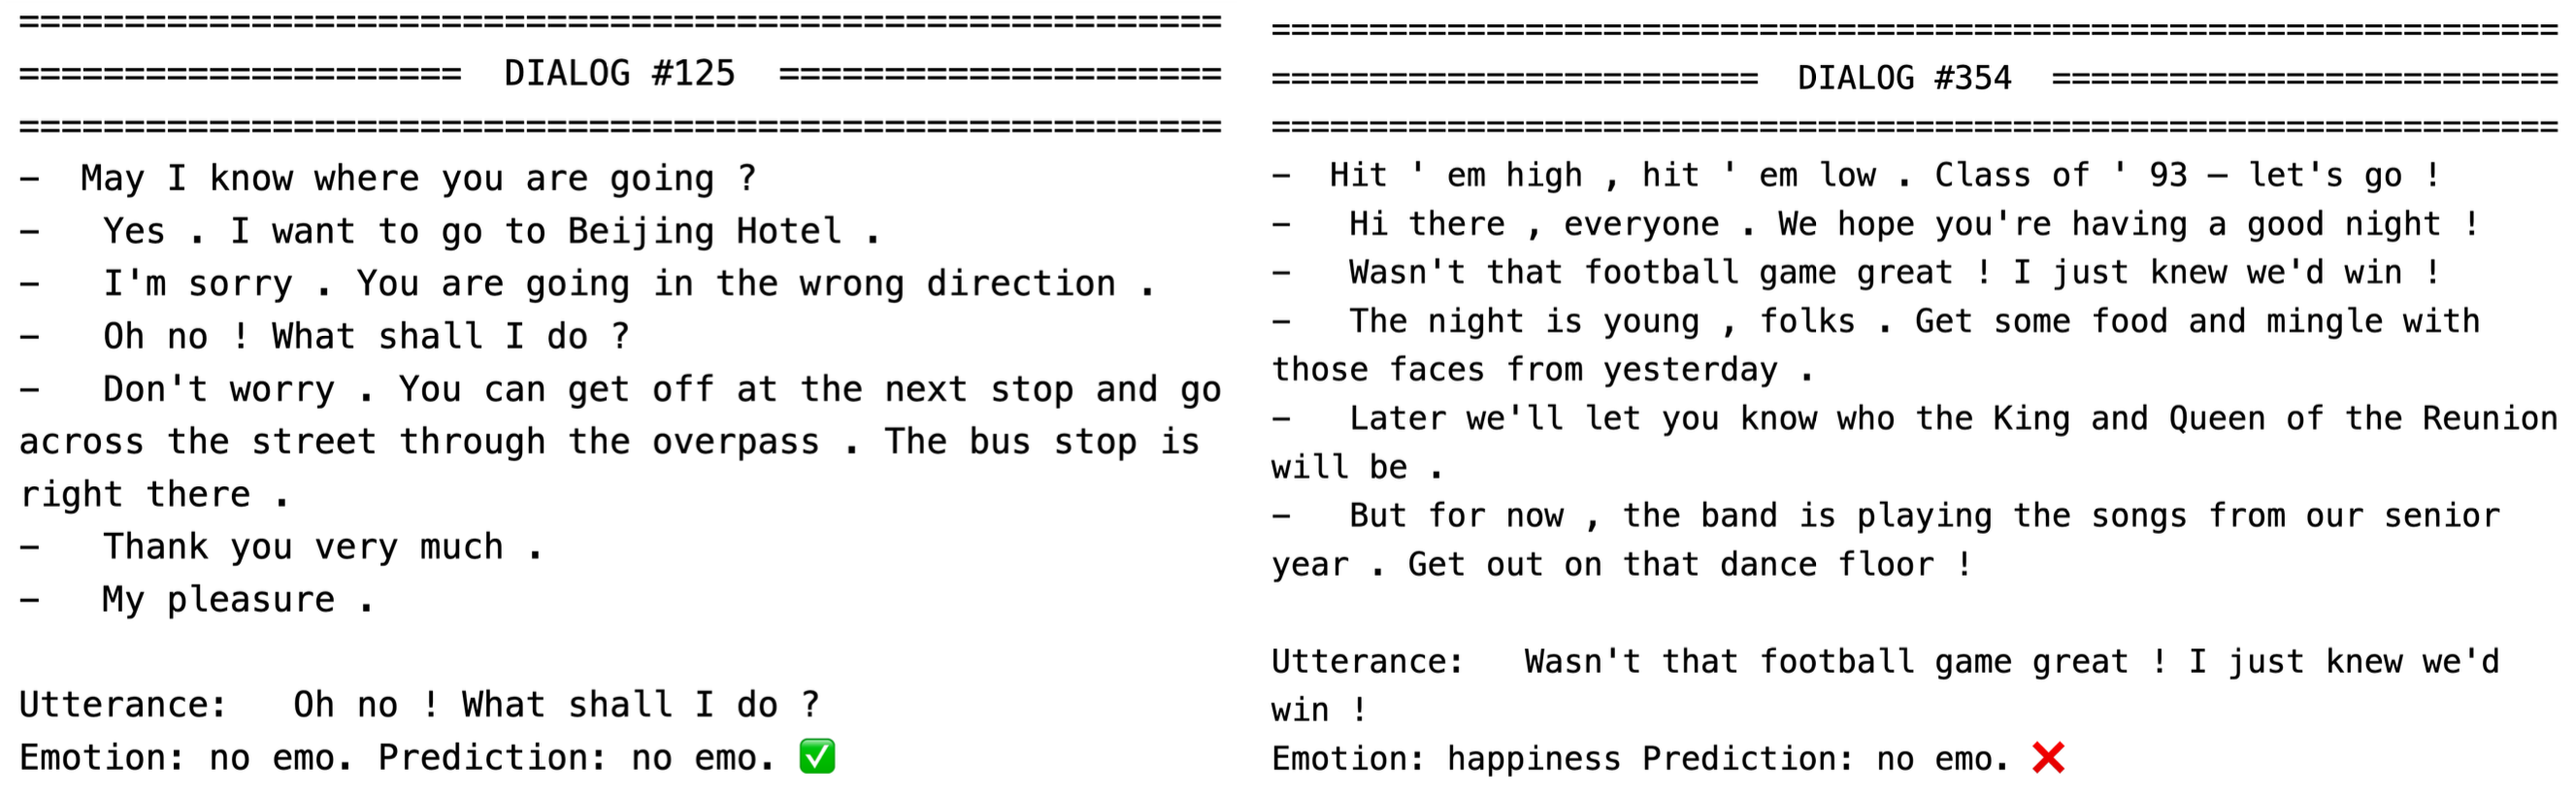
\includegraphics[width=\textwidth]{hsh.png}
        \caption{\centering Deux exemples de prédictions sur des dialogues où le contexte semble être pris en compte (\textsl{à gauche}) et ne pas être utilisé (\textsl{à droite})}
    \end{figure}
\end{frame}

\begin{frame}{Évaluation qualitative}
    \begin{itemize}
        \item Pertinence des prédictions
    \end{itemize}
    % Cela revoie directement à la subjectivité de l'annotation
    \begin{figure}[h]
        \centering
        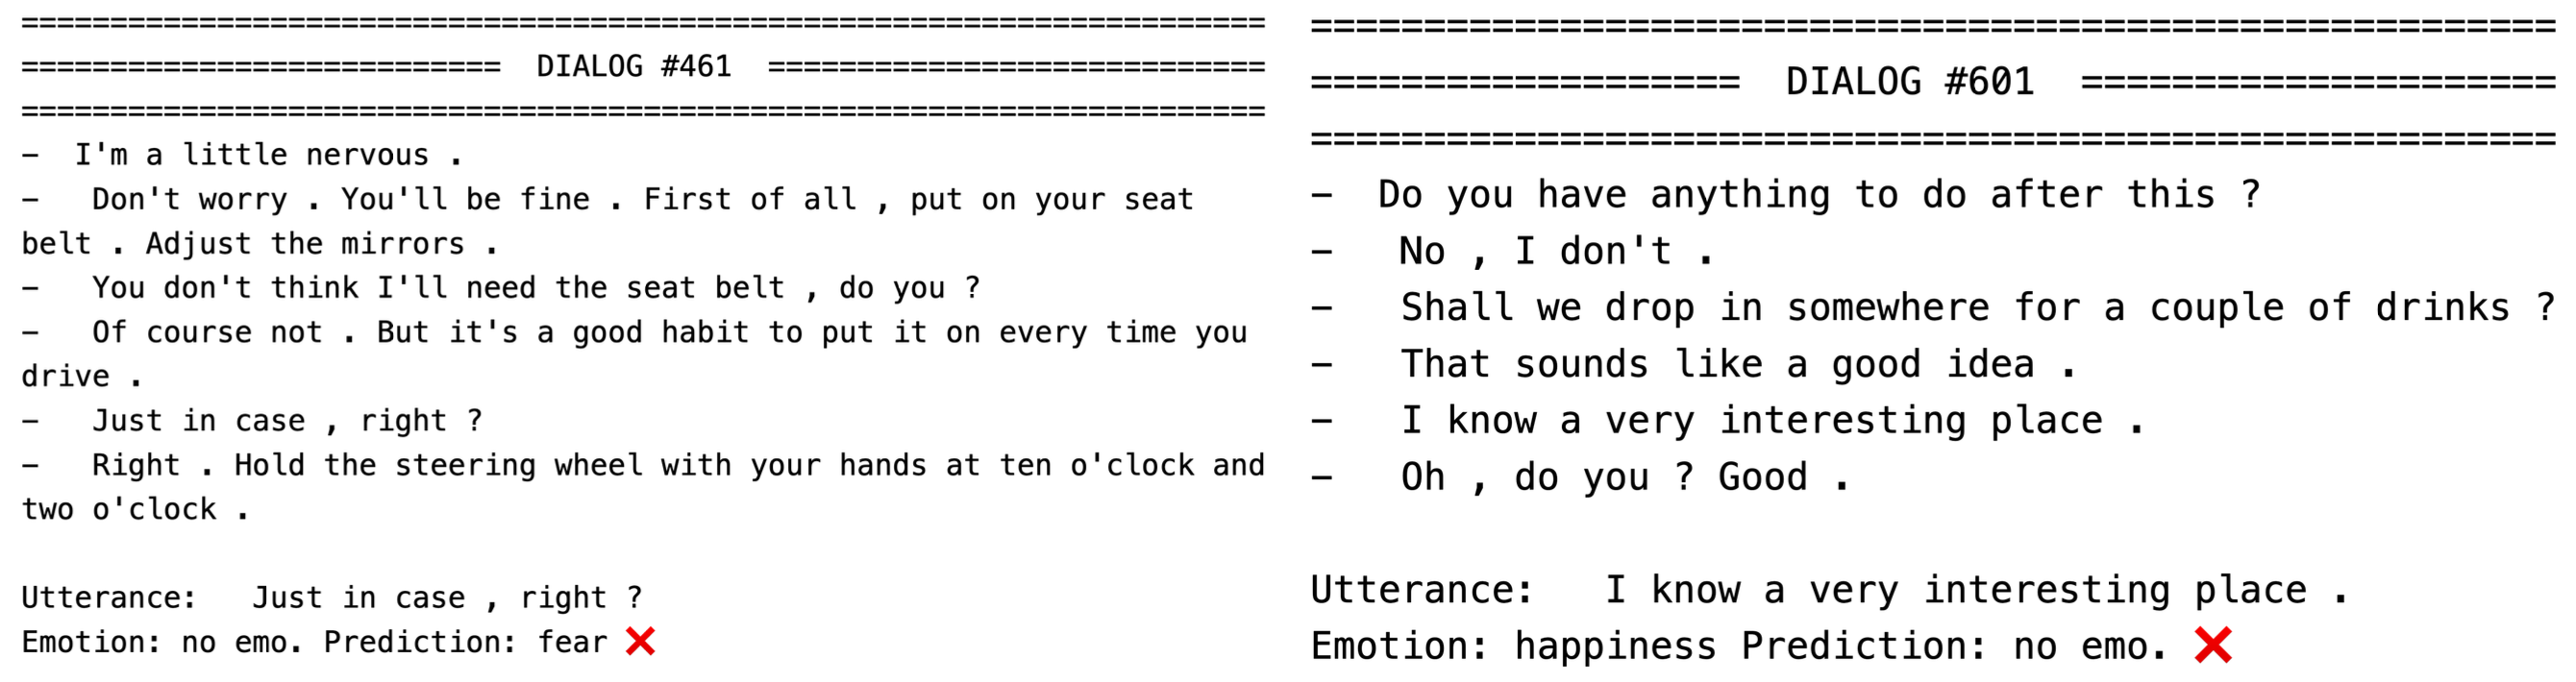
\includegraphics[width=\textwidth]{gp.png}
        \caption{\centering Un exemple de dialogue où une prédiction incorrecte paraît légitime}
    \end{figure}
\end{frame}

\begin{frame}{Comparaison avec les LLMs}
    \begin{figure}
        \centering
        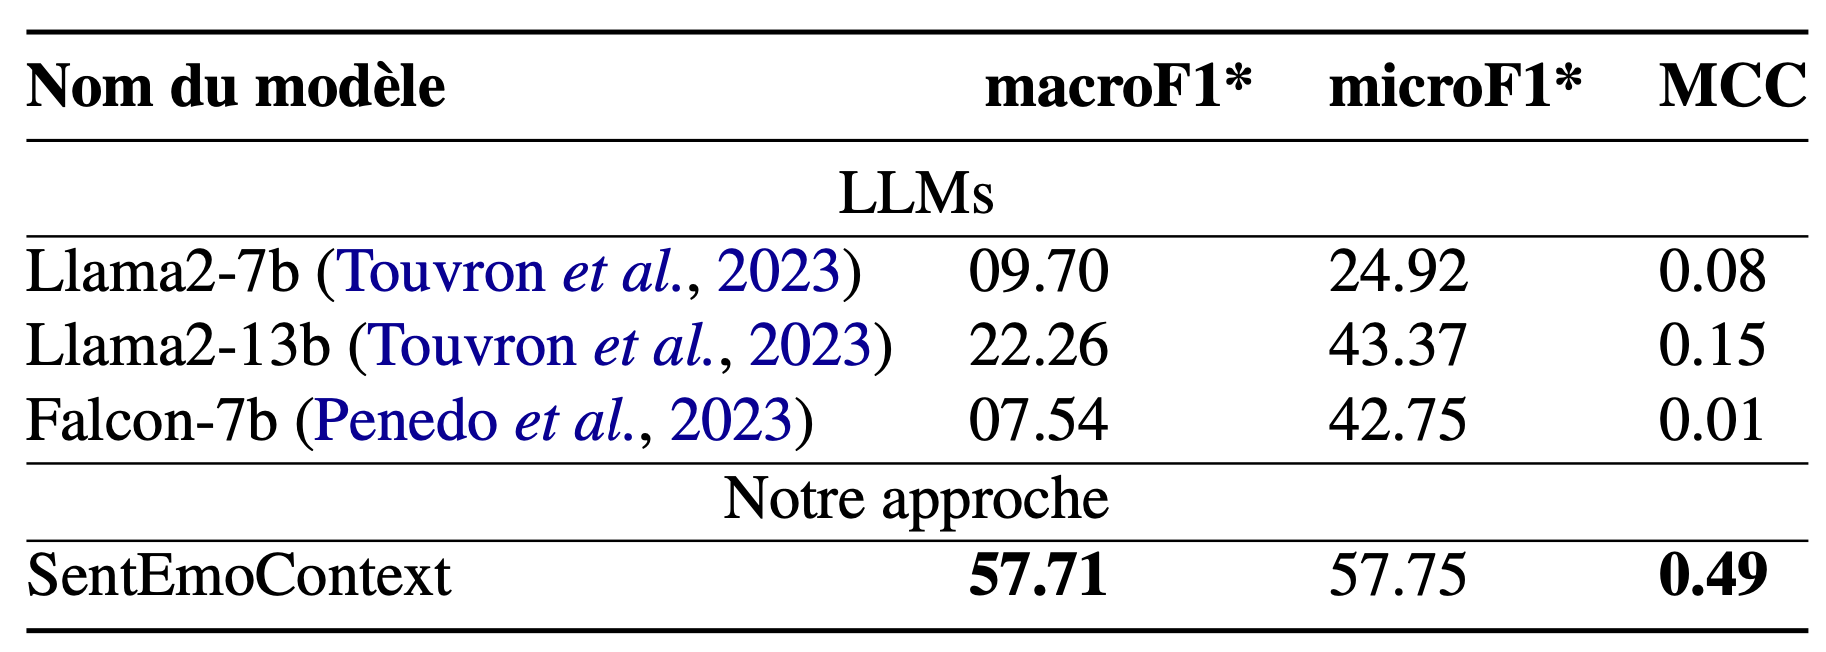
\includegraphics[width=0.6\textwidth]{resultats_llms.png}
        \caption{\centering Résultats avec les LLMs et comparaison avec \texttt{SentEmoContext}}
    \end{figure}
    \begin{figure}
        \centering
        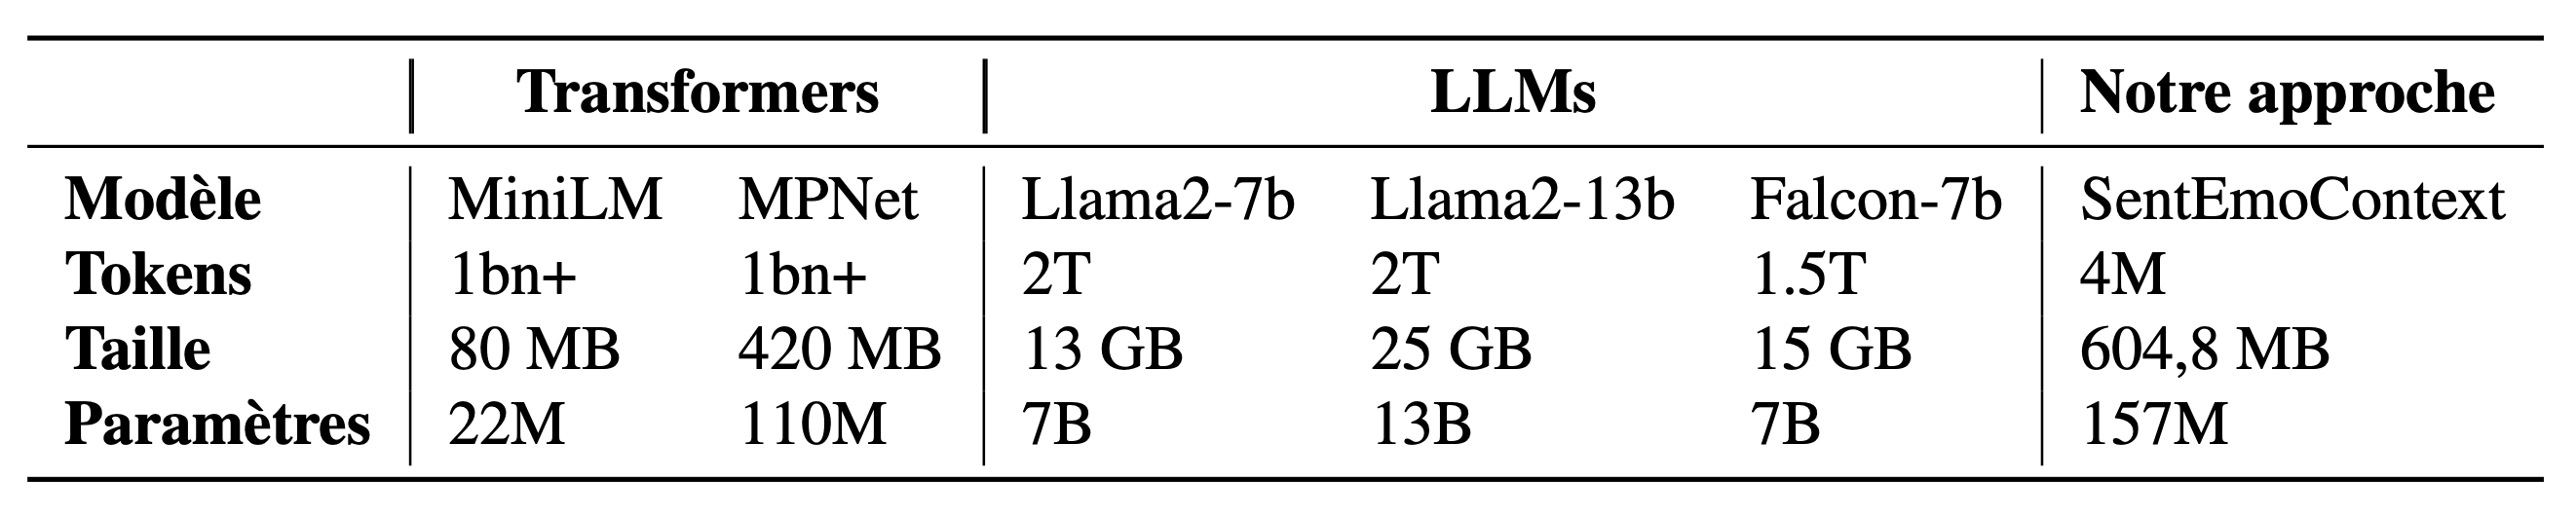
\includegraphics[width=0.7\textwidth]{taille_llms.png}
        \caption{\centering Aperçu de la taille des modèles et comparaison avec \texttt{SentEmoContext}}
    \end{figure}
\end{frame}

\section{Conclusion}

\begin{frame}{Conclusion}
% Retour sur les questions de recherche :    
\textcolor{roose}{\bf RQ1:} Comment utiliser l'information provenant du contexte conversationnel pour guider la détection d'émotions en conversation ?
    \begin{itemize}
        \item Déployer de l'attention à l'échelle du dialogue
        \item Modification des représentations des propos
    \end{itemize}
\vspace{10pt}
\visible<2->{
\textcolor{roose}{\bf RQ2:} Est-ce que la prise en compte du contexte conversationnel permet d'améliorer la détection d'émotions en conversation dans le cas dyadique ?
    \begin{itemize}
        \item Enjeu de la stabilité du modèle
        \item Déployer l'attention engendre du bruit et propage les émotions
    \end{itemize}
}
\end{frame}

\begin{frame}{Perspectives}
    \begin{columns}
        \begin{column}[c]{0.4\linewidth}
            \begin{itemize}
                \item Prédictions sur des étiquettes émotionnelles inconnues du modèle
                \item Enrichissement des données d'entraînement pour améliorer la stabilité du modèle (exemple: \texttt{EmpatheticDialogues}~\manualcite{Rashkin et al., 2019}) 
            \end{itemize}
        \end{column}
        \begin{column}[c]{0.5\linewidth}
            \begin{figure}
                \centering
                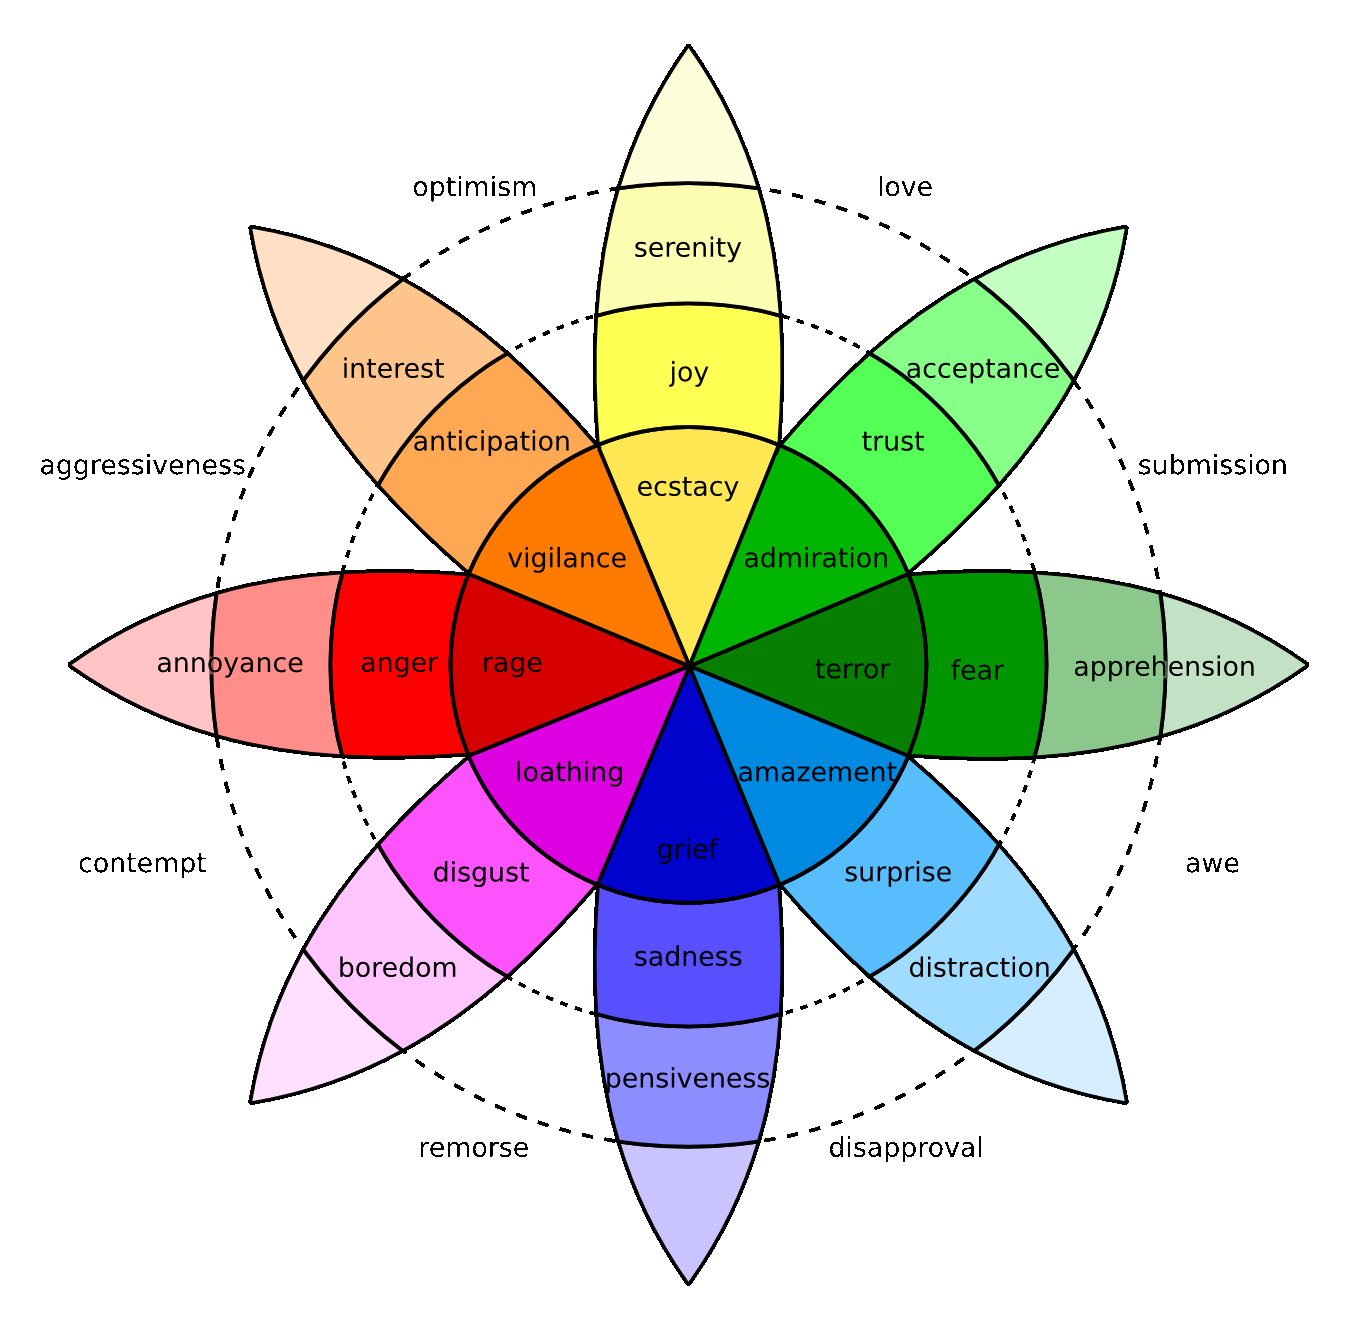
\includegraphics[width=0.6\textwidth]{emotion_wheel.png}
                \caption{\centering Roue des émotions de Plutchik~\manualcite{Plutchik, 2001}}
            \end{figure}
        \end{column}
    \end{columns}
\end{frame}


\begin{frame}[plain]
    \begin{center}
        \vspace{0.2cm}
        {\color{deepblue}\Huge Merci pour votre attention !}
        
        \vspace{0.5cm}
        
        \begin{figure}[h]
            \centering
            \begin{minipage}{0.45\textwidth}
                \centering
                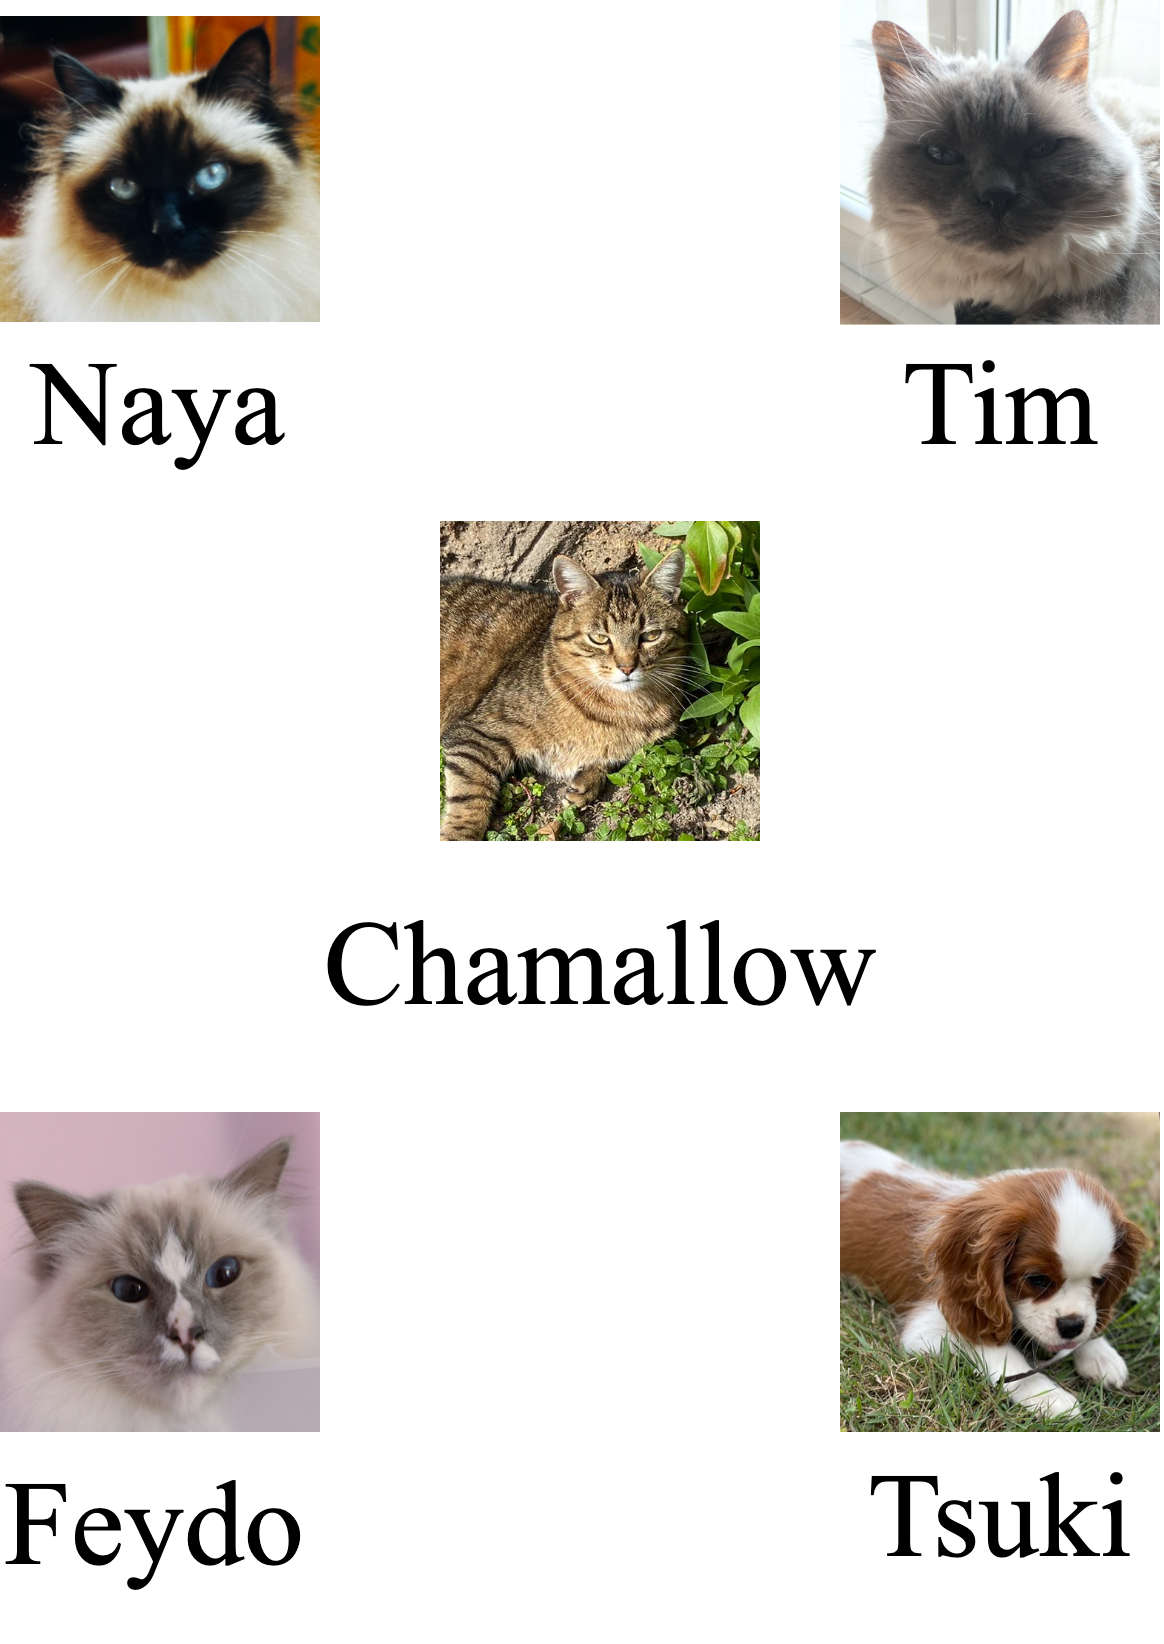
\includegraphics[width=0.6\textwidth]{animals.png}
                \caption{Les animaux (page 2)}
            \end{minipage}
            \hspace{0.05\textwidth}
            \begin{minipage}{0.45\textwidth}
                \centering
                
\includegraphics[width=0.8\textwidth]{code-gh.png}
                \caption{\centering Code : \url{https://github.com/B-Gendron/sentEmoContext}}
            \end{minipage}
        \end{figure}
    \end{center}
\end{frame}

\section{Références}

\begin{frame}[t,allowframebreaks,noframenumbering]
\frametitle{Références}
\printbibliography
\end{frame}

\begin{frame}[noframenumbering]
    \frametitle{Crédits illustrations}
    \textbf{Animaux en page 2}
    \begin{itemize}
        \item félins : \url{https://www.hachette.fr/livre/decouvre-le-monde-felins-9782017074717}
        \item canidés : \url{https://www.livres-medicaux.com/sante-tout-public/20544-canides-du-monde-loups-chiens-sauvages-renards-chacals-coyotes-et-apparentes.html}
        \item loup arctique : \url{https://www.josephfiler.com/photo/canada-arctic-wolf-0348/}
        \item tigre : \url{https://evasion-online.com/tag/tigre}
        \item tigreau : \url{http://www.trouver-tout.fr/bebe-tigre-blanc/}
        \item caracal : \url{https://fr.wikipedia.org/wiki/Caracal}
        \item lionne : \url{https://www.futura-sciences.com/fonds-ecran/lion-lionne-lionceaux-1625/}
        \item renard : \url{http://eliotkitty.centerblog.net/27563-Magnifique-renard}
    \end{itemize}
    \end{frame}

% ========================================================
% =====================  APPENDIX  =======================
% ========================================================

\appendix

\begin{frame}[plain, noframenumbering]{About Classification Metrics}
    Given:
    \begin{itemize}
        \item $P$ the quantity of positive predictions
        \item $N$ the quantity of negative predictions
        \item $\mathit{TP}$, $\mathit{TN}$, $\mathit{FP}$ and $\mathit{FN}$ the True Positives, True Negatives, False Positives and False Negatives
    \end{itemize}
        \begin{align}
        \text{Accuracy} & = \dfrac{\mathit{TP} + \mathit{TN}}{P+N} \quad
        \text{Precision} = \dfrac{\mathit{TP}}{\mathit{TP}+\mathit{FP}} \\[0.5ex]
        \text{Recall} & = \dfrac{\mathit{TP}}{\mathit{TP}+\mathit{FN}}\quad 
        \text{F}_1 = \dfrac{2\mathit{TP}}{2\mathit{TP}+\mathit{FP}+\mathit{FN}}
    \end{align}
    \end{frame}
    
    \begin{frame}[plain, noframenumbering]{About Matthews Correlation Coefficient (MCC) \textcolor{gray}{\footnotesize (Cramér, 1946)}}
        Given:
        \begin{equation}
    N = \mathit{TN}+\mathit{TP}+\mathit{FN}+\mathit{FP} \enspace \text{,} \quad S = \frac{\mathit{TP}+\mathit{FN}}{N} \enspace \text{and} \quad P = \frac{\mathit{TP}+\mathit{FP}}{N}
    \end{equation}
    
    MCC has been defined in \textcolor{gray}{\footnotesize (Matthews,~1975)} as:
    
    \begin{equation}
        \text{MCC} = \frac{\mathit{TP}/ N-S \times P}{\sqrt{P S(1-S)(1-P)}}
    \end{equation}
    \end{frame}
        
    
    \begin{frame}[plain, noframenumbering]{Distribution of emotions within the dialog}
        \begin{figure}
        \centering
        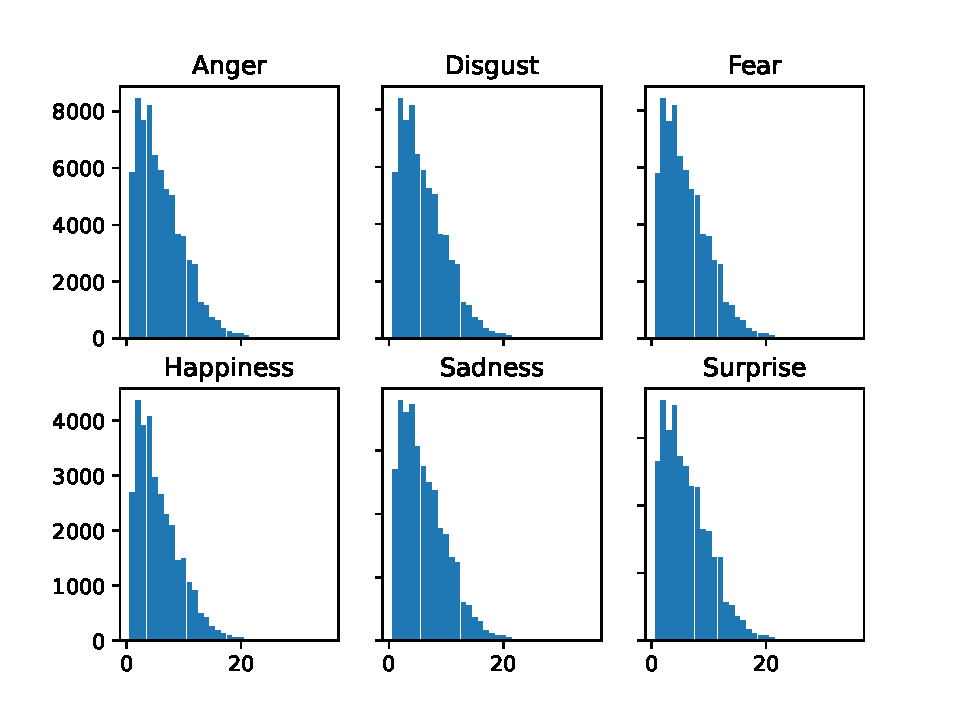
\includegraphics[scale=0.55]{figures/emo_dist_sp_6_labelled.pdf}
        \caption{\centering Cumulative number of expressed emotions \textit{w.r.t.} the utterance index}
        \label{fig:emo_dist_6}
    \end{figure}
    \end{frame}

    \begin{frame}[plain, noframenumbering]{Prompt examples}
        \begin{figure}
            \centering
            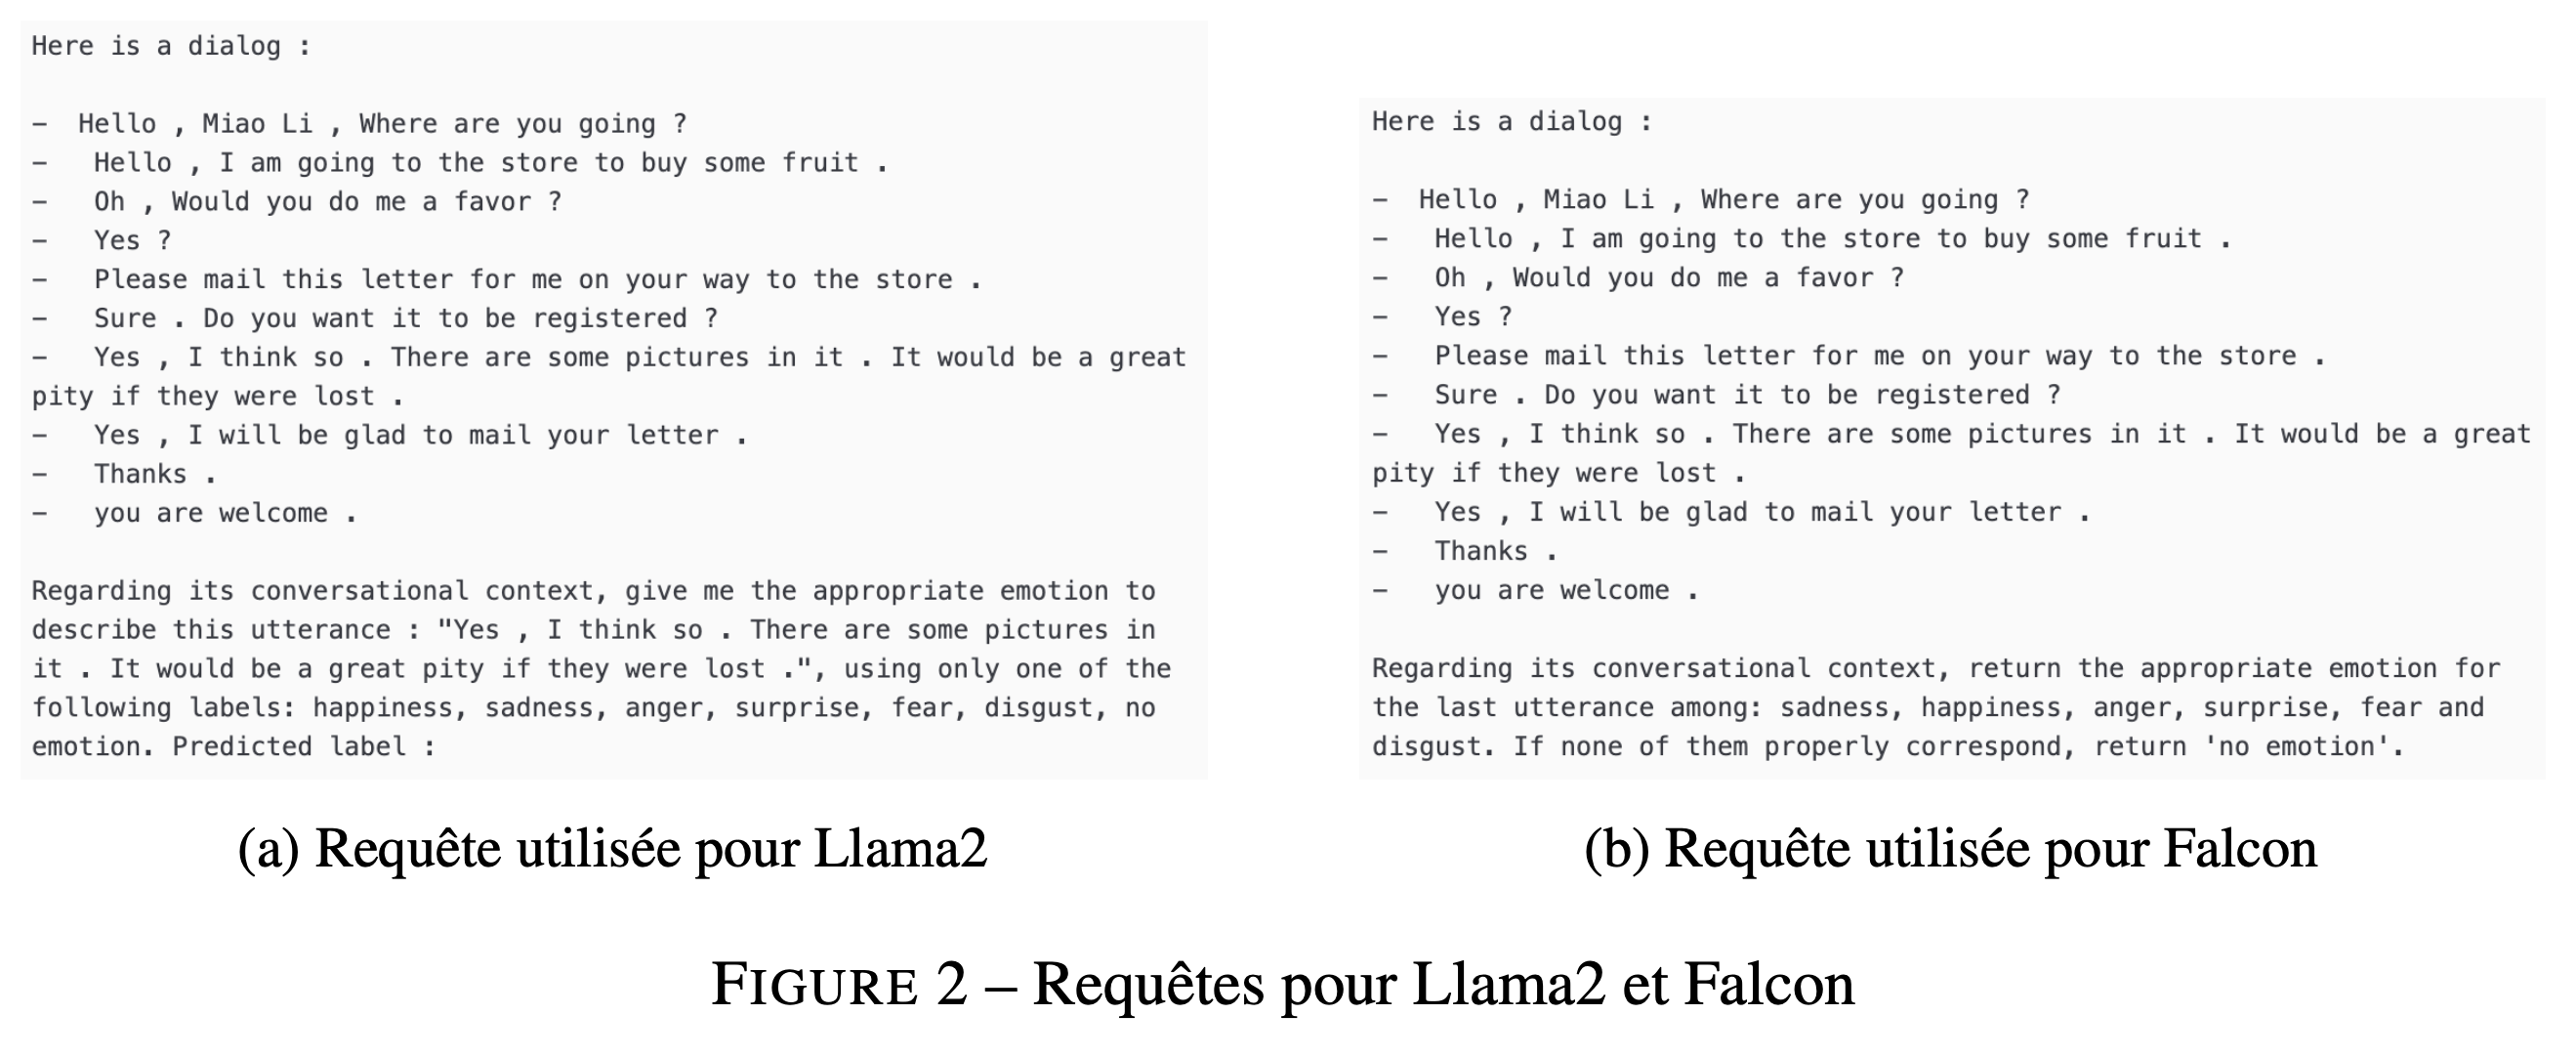
\includegraphics[width=\textwidth]{prompts.png}
        \end{figure}
    \end{frame}
    
    \begin{frame}[plain, noframenumbering]{Some unexplainable predictions}
        \begin{figure}
            \centering
            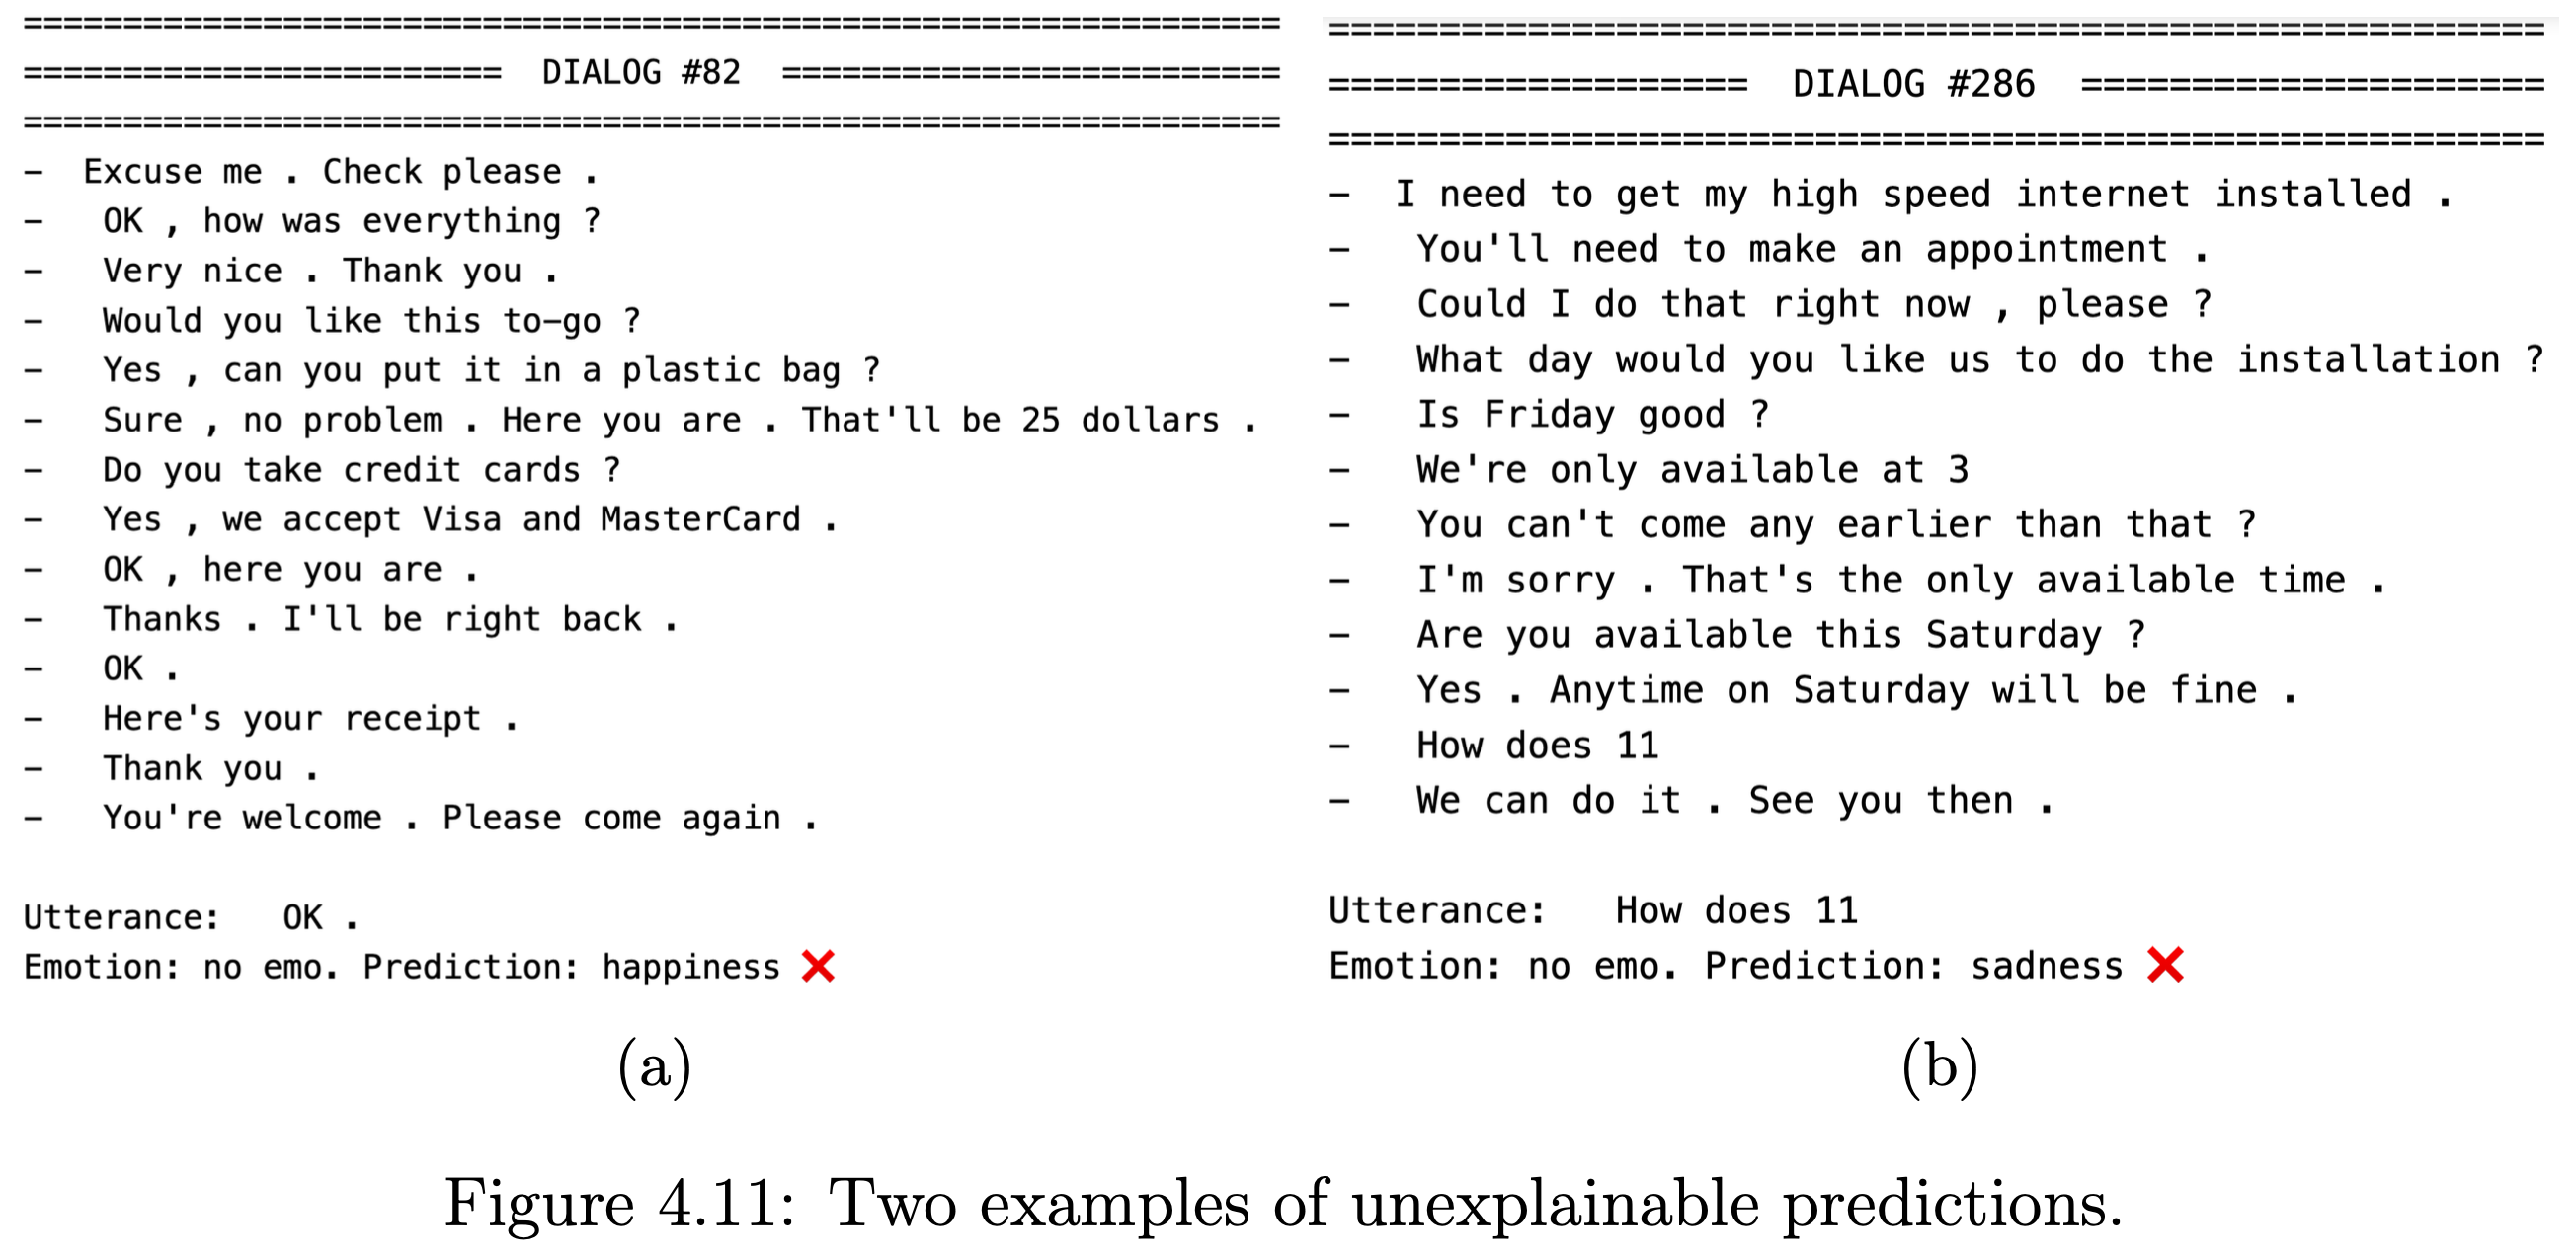
\includegraphics[width=\textwidth]{figures/wtf.png}
            \label{fig:wtf}
        \end{figure}
    \end{frame}
    
    \begin{frame}[plain, noframenumbering]{Preprocessing Pipeline}
        \begin{figure}
        \centering
        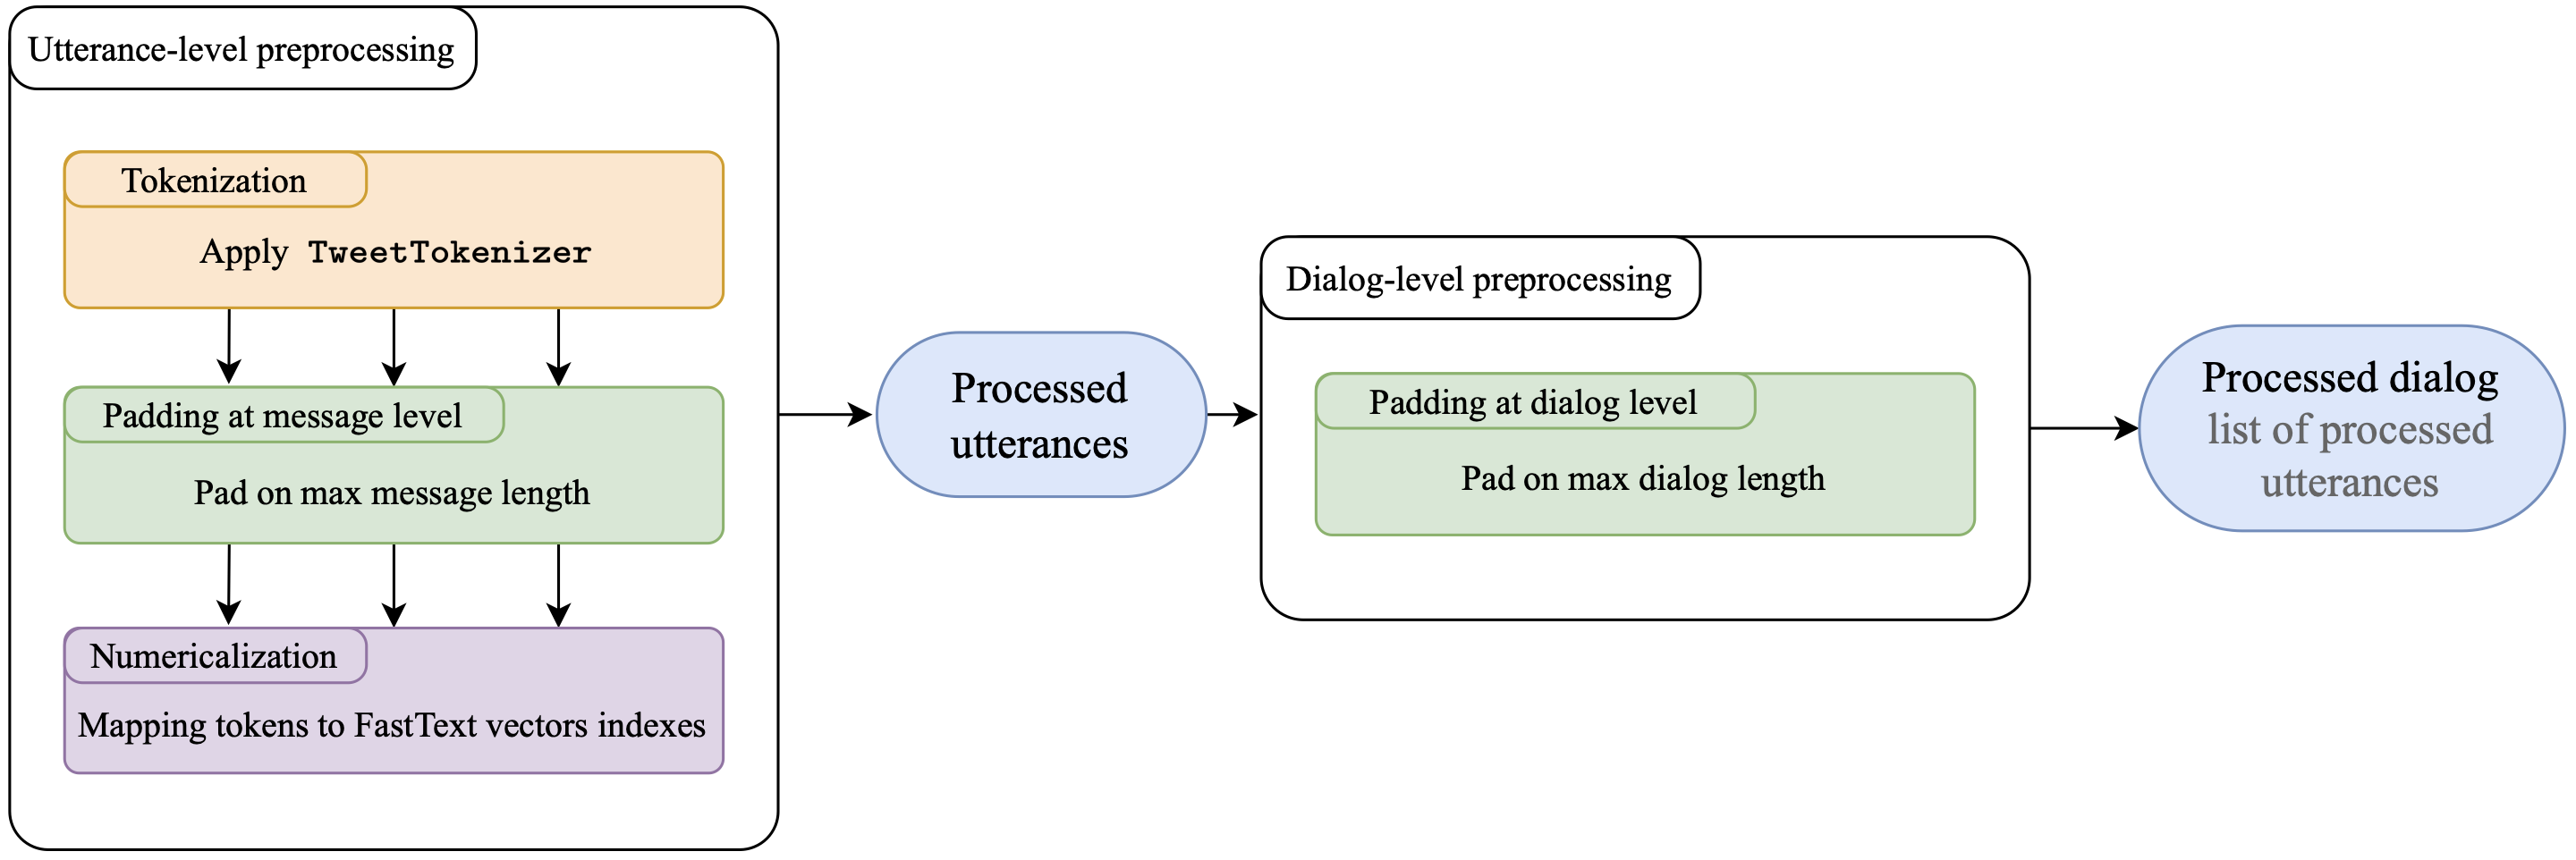
\includegraphics[width=\textwidth]{figures/preproc_static2.png}
        \label{fig:preproc_pipeline_isolated2}
        \caption{\centering Preprocessing steps for isolated utterance representations}
    \end{figure}
    \end{frame}
    
    \begin{frame}[plain, noframenumbering]{Preprocessing Pipeline}
        \begin{figure}
        \centering
        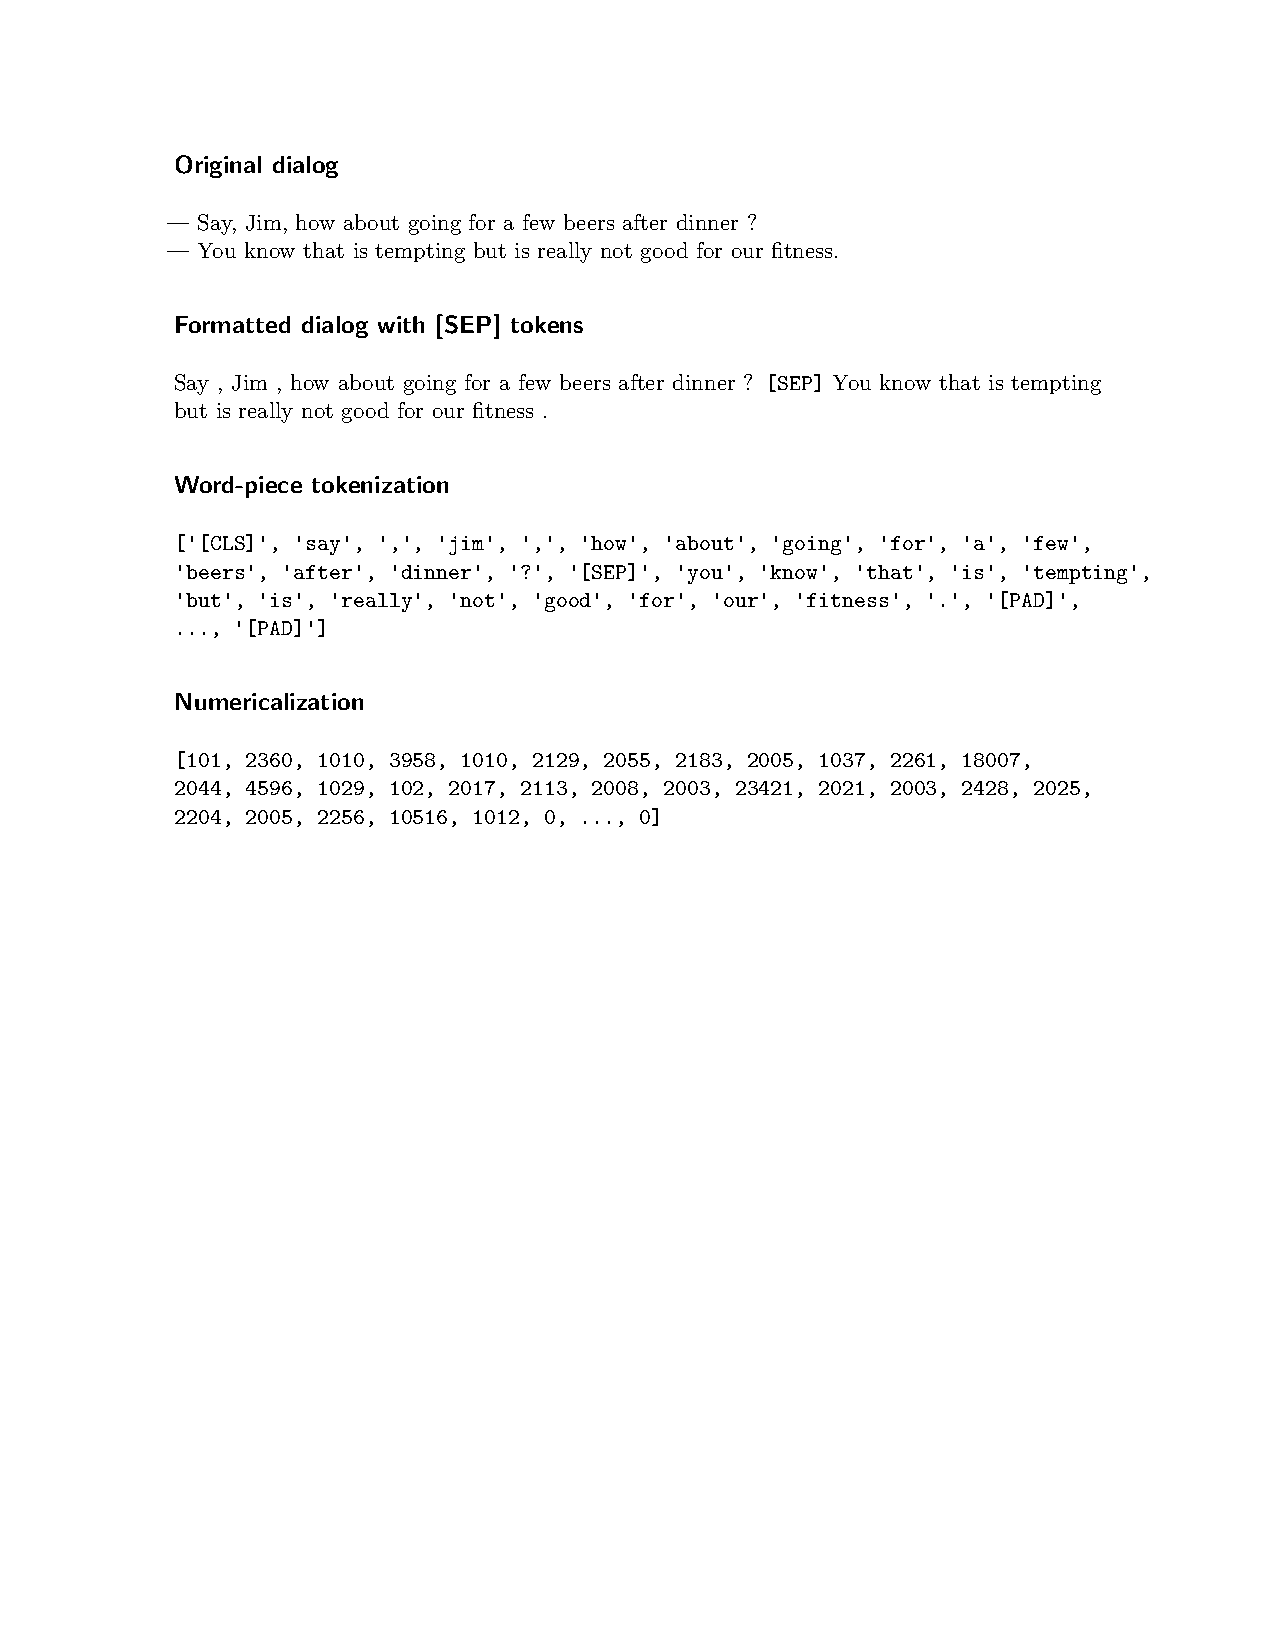
\includegraphics[scale=0.56]{figures/bert-output-simple.pdf}
        \label{fig:preproc_context_example4}
    \end{figure}
    \end{frame}
    
    \begin{frame}[plain, noframenumbering]{Prediction Distributions - Isolated Utterances}
        \begin{figure}[!ht]
        \centering
    \begin{subfigure}{0.18\textwidth}
      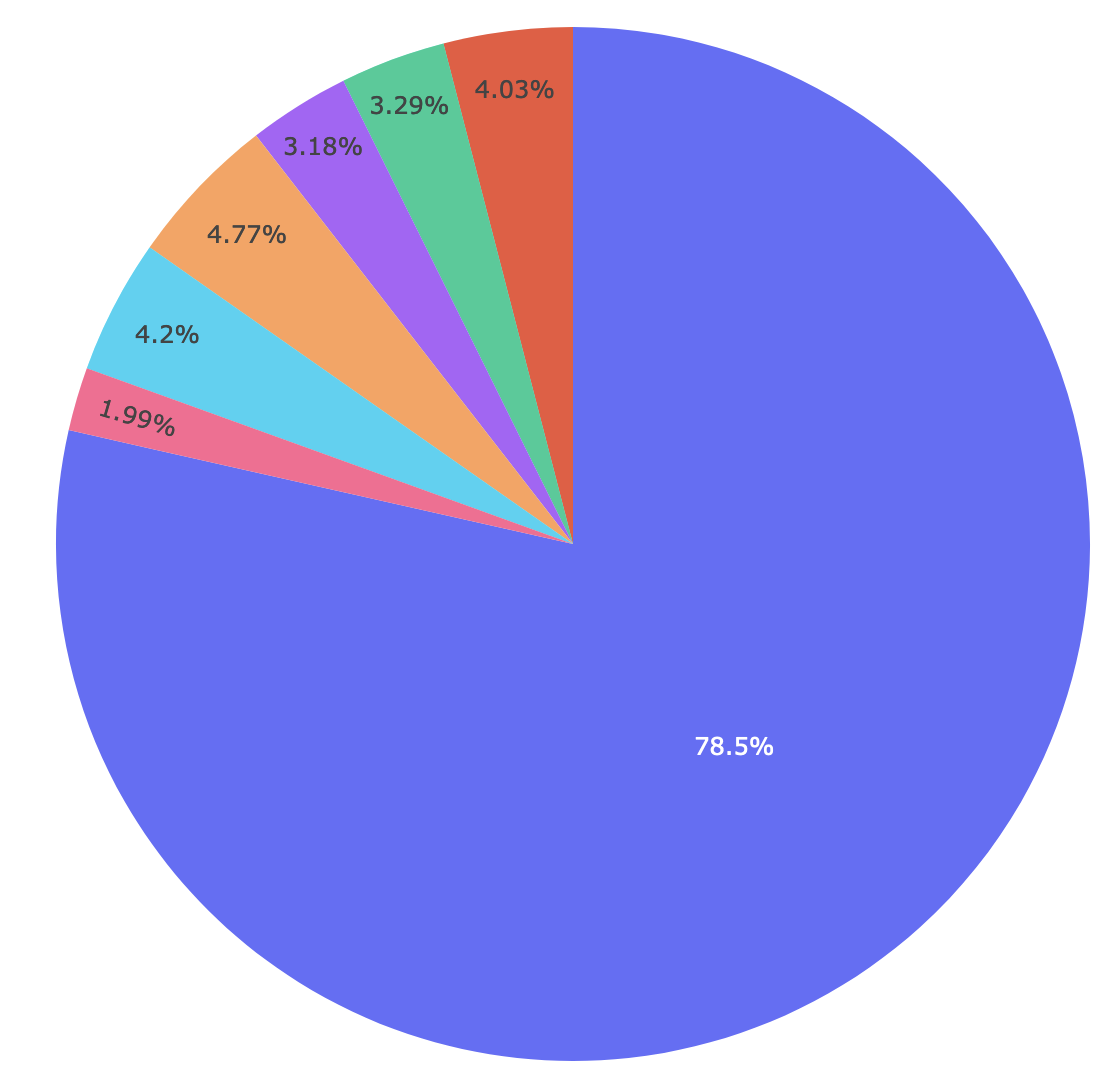
\includegraphics[width=\linewidth]{figures/no-emotion.png}
      \caption*{No emotion}
    \end{subfigure}\hfil
    \begin{subfigure}{0.18\textwidth}
      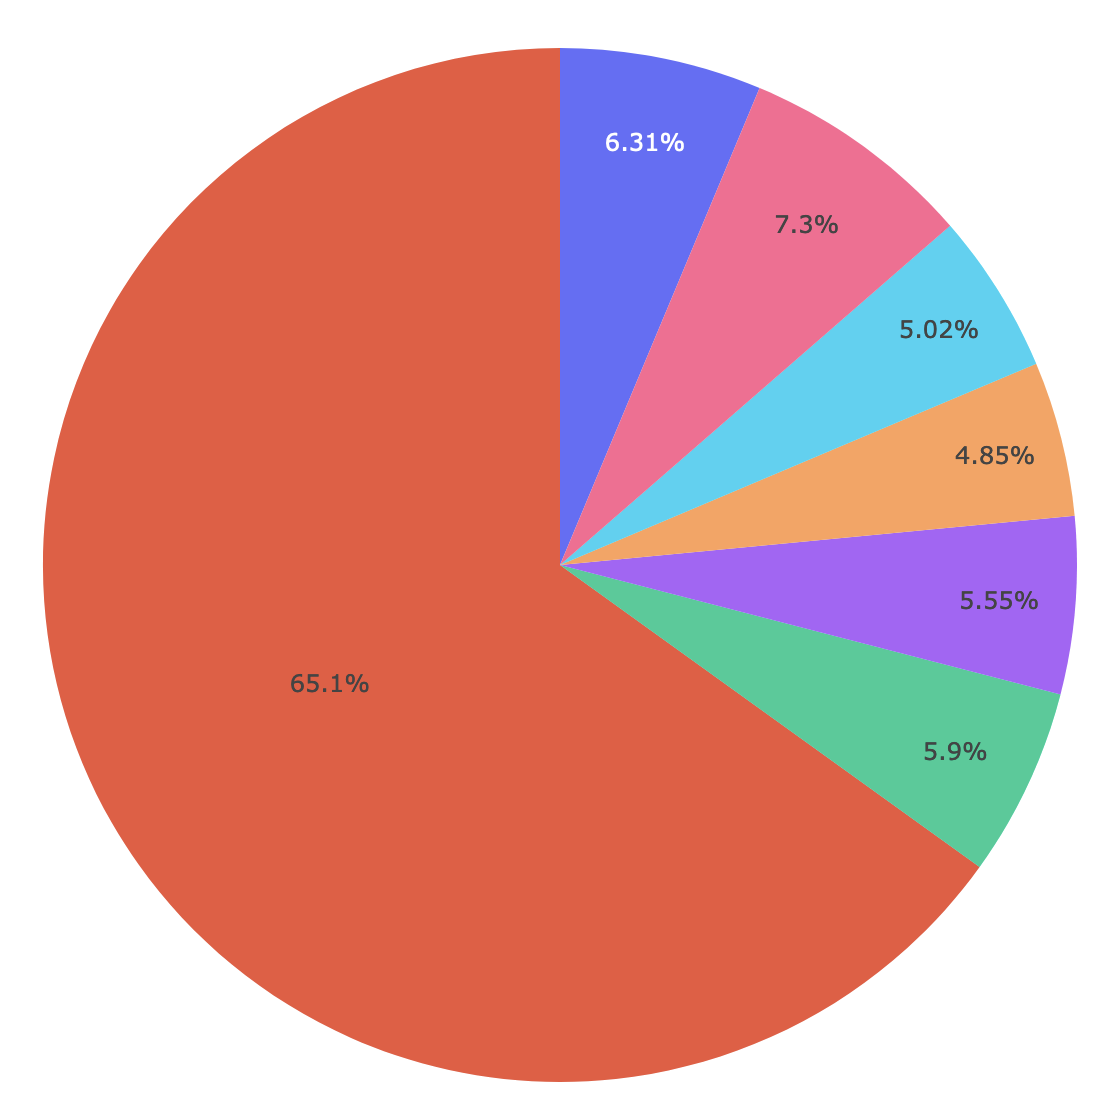
\includegraphics[width=\linewidth]{figures/anger.png}
      \caption*{Anger}
    \end{subfigure}\hfil
    \begin{subfigure}{0.18\textwidth}
      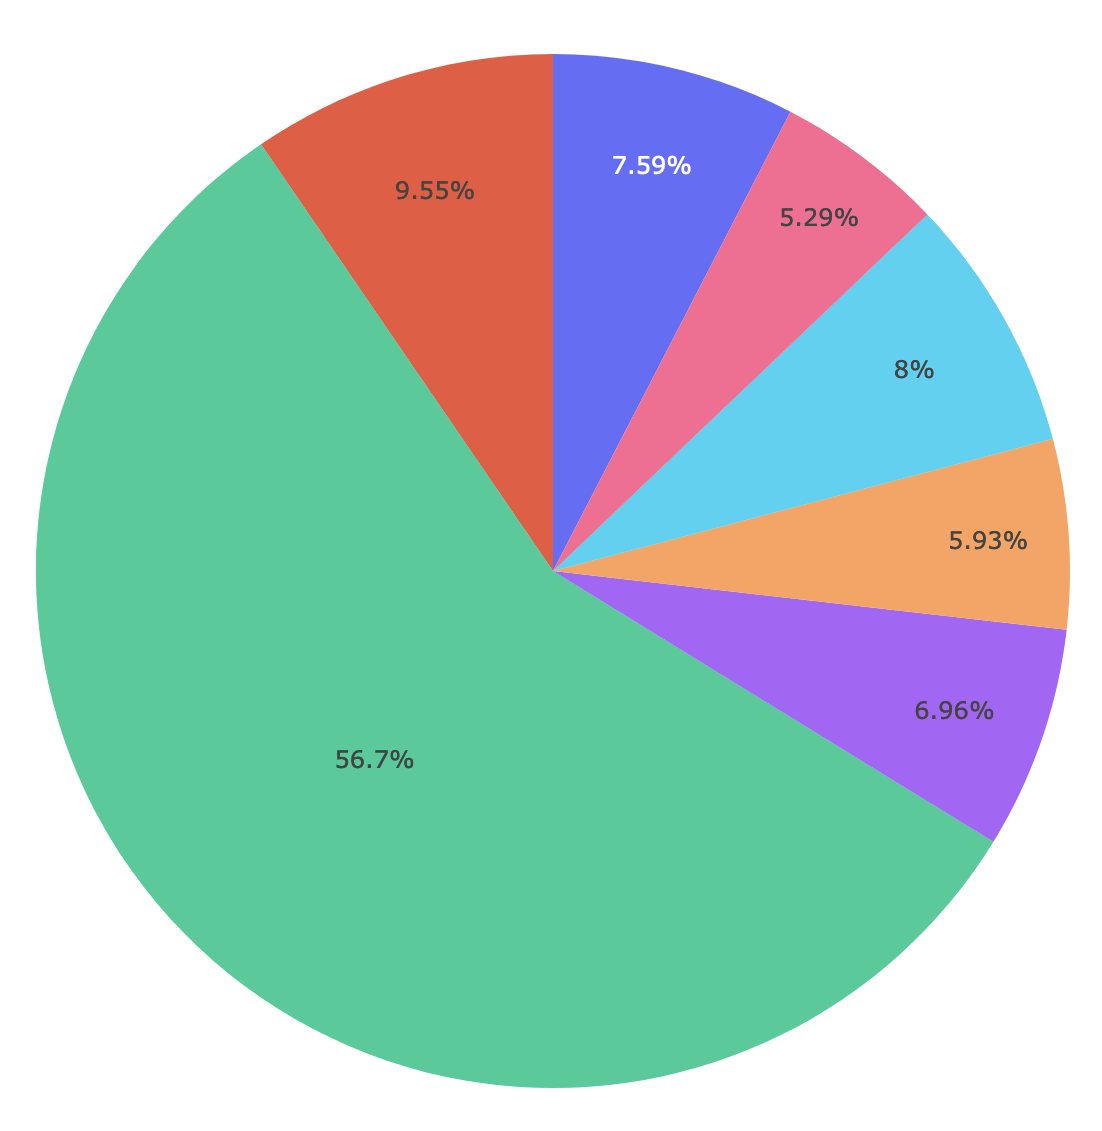
\includegraphics[width=\linewidth]{figures/disgust.png}
      \caption*{Disgust}
    \end{subfigure}\hfil
    \begin{subfigure}{0.18\textwidth}
      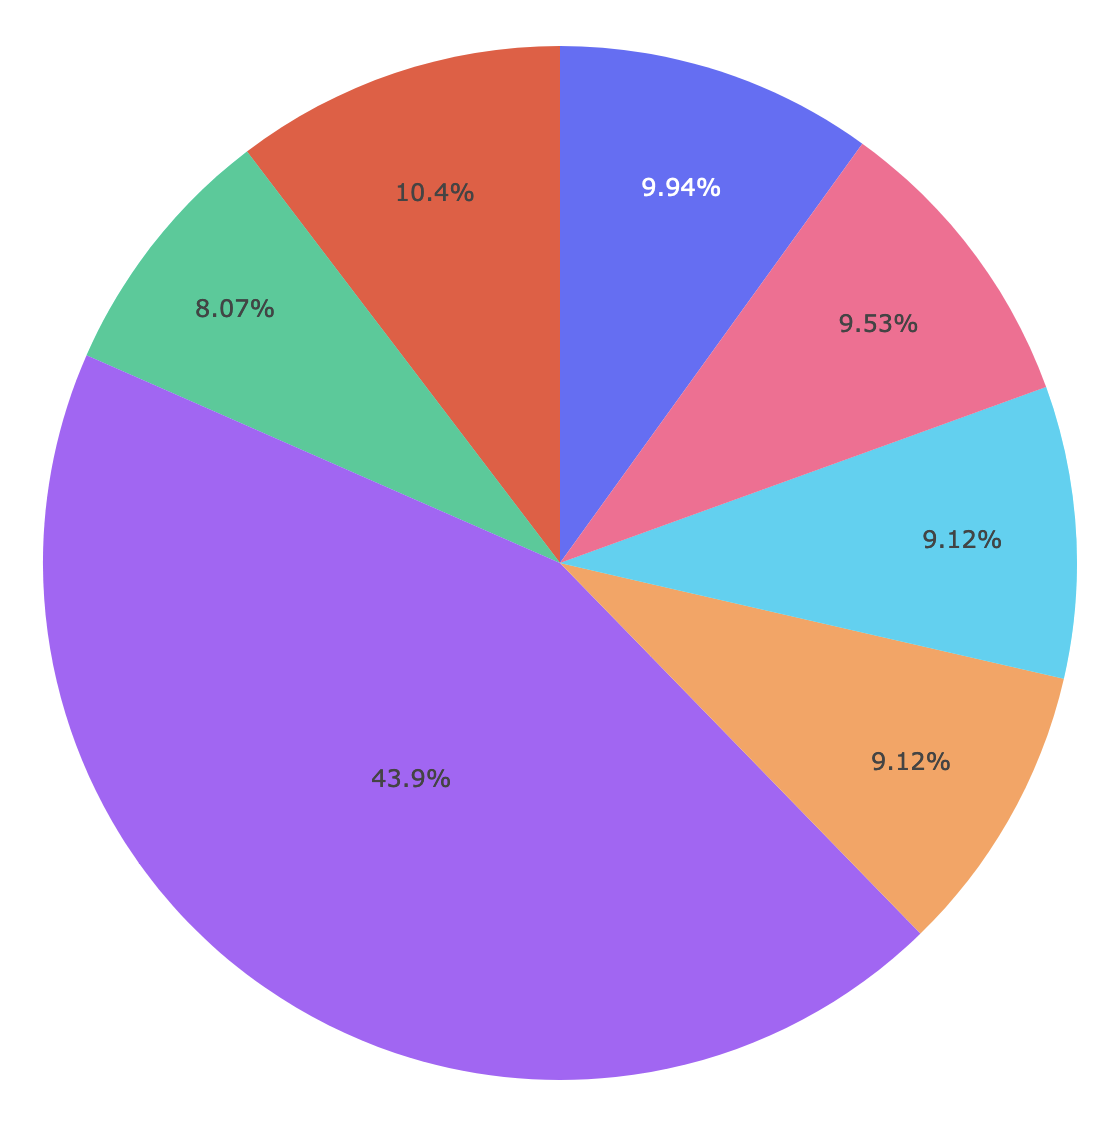
\includegraphics[width=\linewidth]{figures/fear.png}
      \caption*{Fear}
    \end{subfigure}
    
    \medskip
    \begin{subfigure}{0.18\textwidth}
      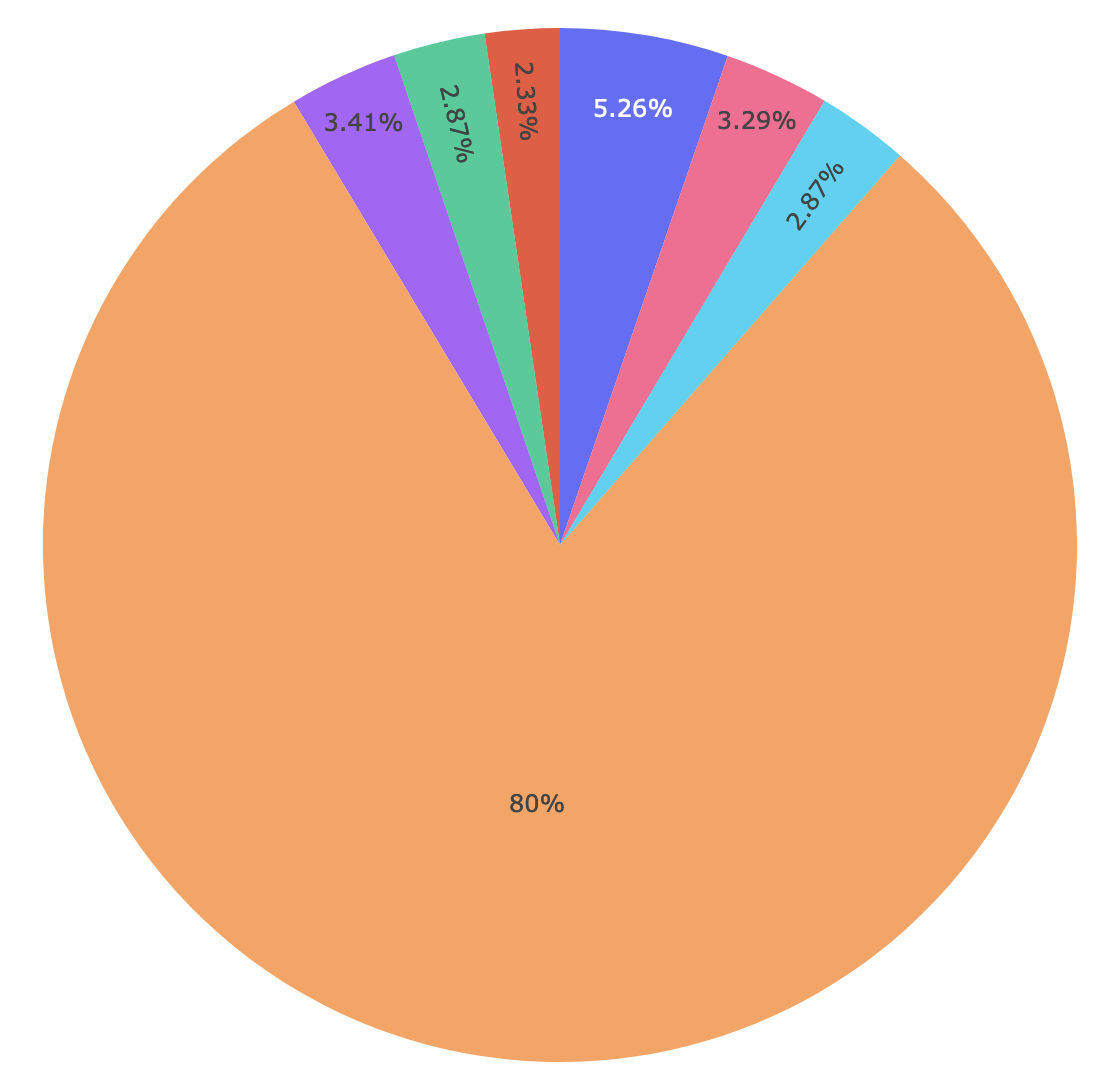
\includegraphics[width=\linewidth]{figures/happiness.png}
      \caption*{Happiness}
    \end{subfigure}\hfil 
    \begin{subfigure}{0.18\textwidth}
      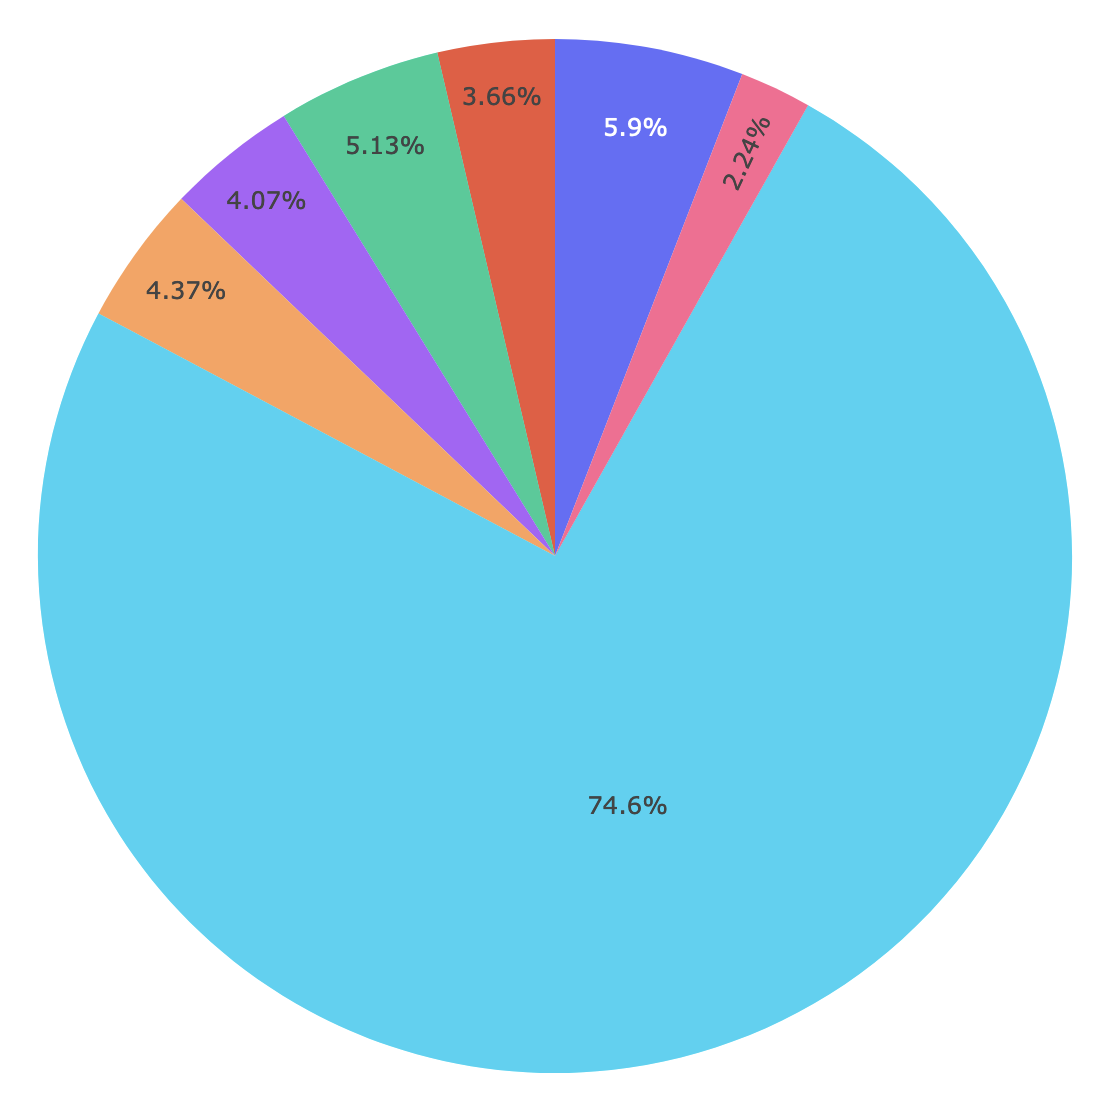
\includegraphics[width=\linewidth]{figures/sadness.png}
      \caption*{Sadness}
    \end{subfigure}\hfil 
    \begin{subfigure}{0.18\textwidth}
      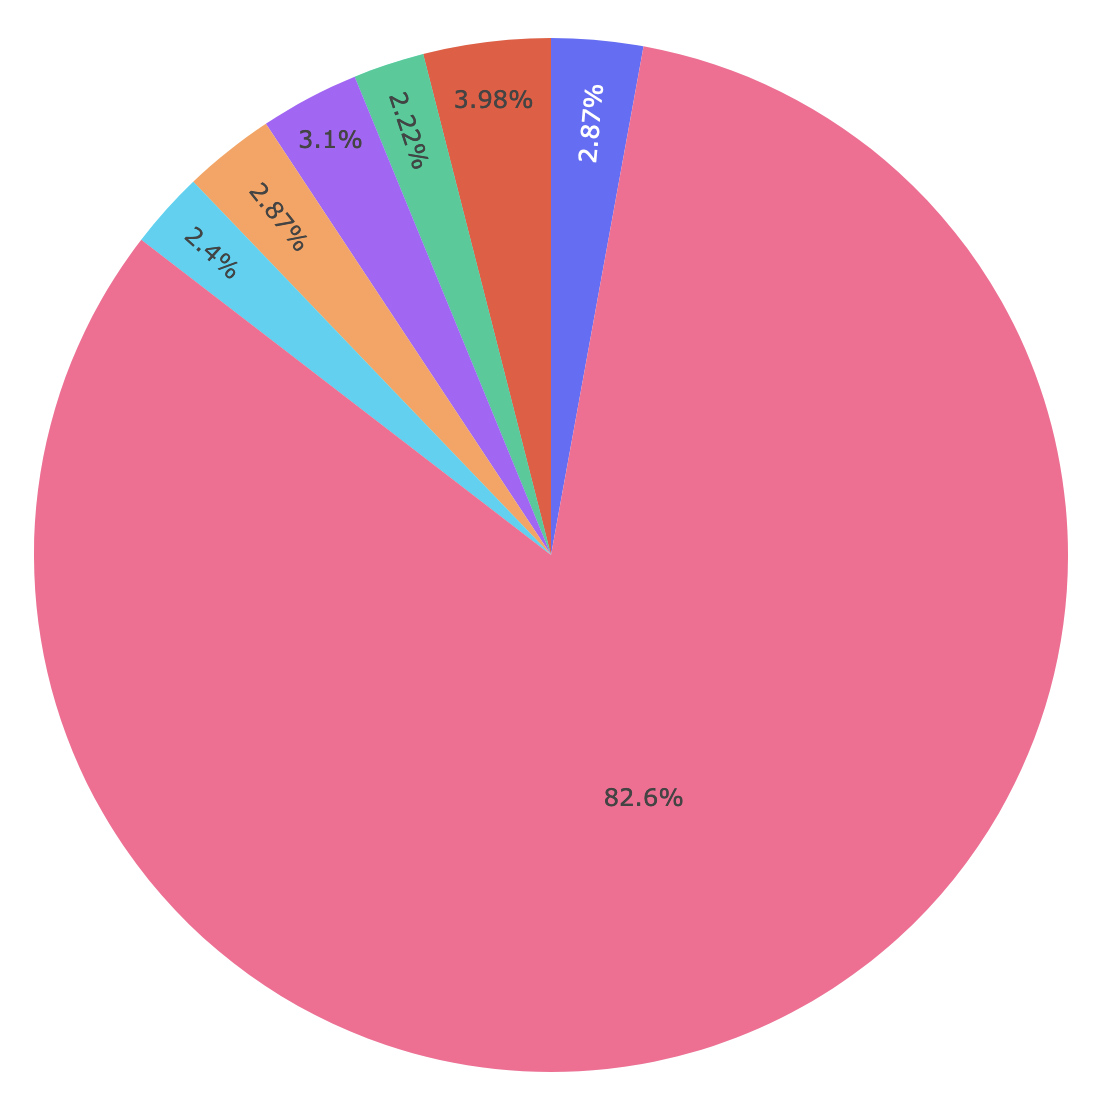
\includegraphics[width=\linewidth]{figures/surprise.png}
      \caption*{Surprise}
    \end{subfigure}\hfil
    \begin{subfigure}{0.18\textwidth}
      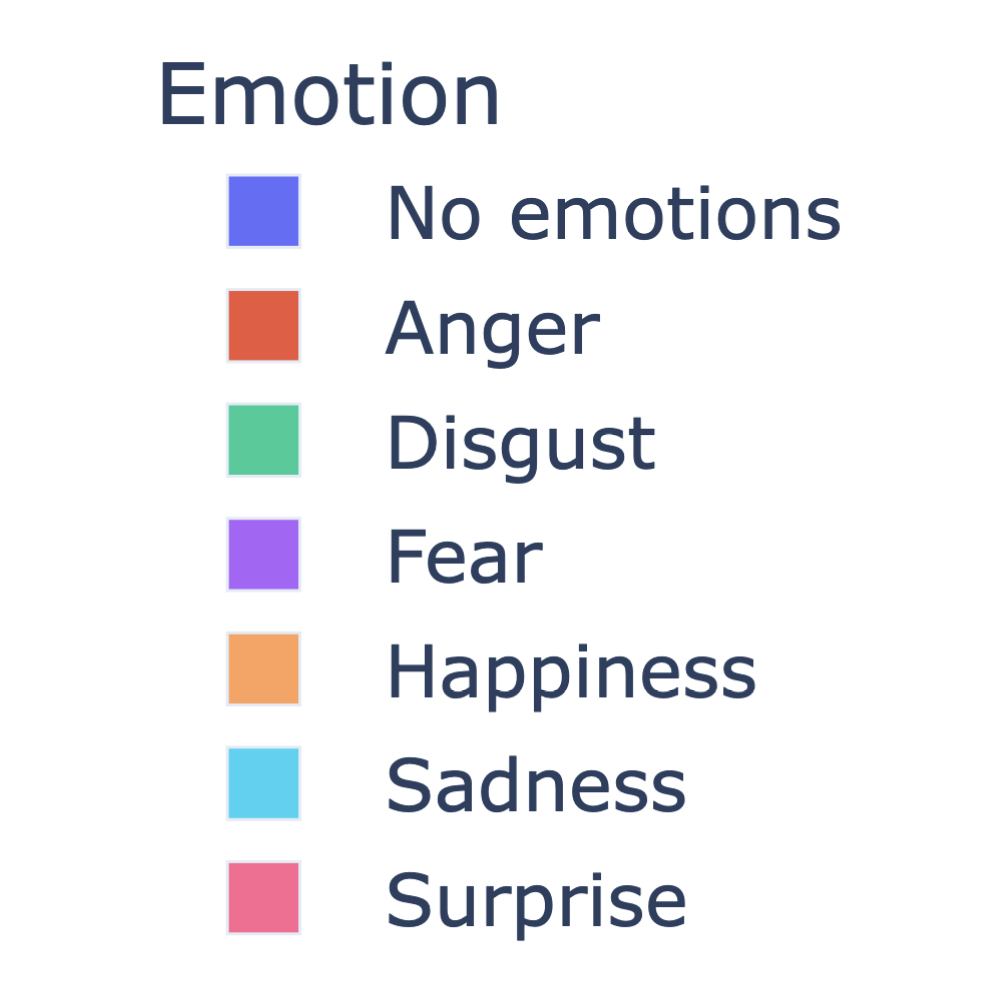
\includegraphics[width=\linewidth]{figures/legend.png}
      \caption*{}
    \end{subfigure}
    % \caption{\centering Distribution of predictions for each actual emotion in the case of isolated utterances representations.}
    \label{fig:pred_distrib}
    \end{figure}
    \end{frame}
    
    \begin{frame}[plain, noframenumbering]{Prediction Distributions - Contextual Utterances}
    \begin{figure}[!ht]
        \centering
    \begin{subfigure}{0.19\textwidth}
      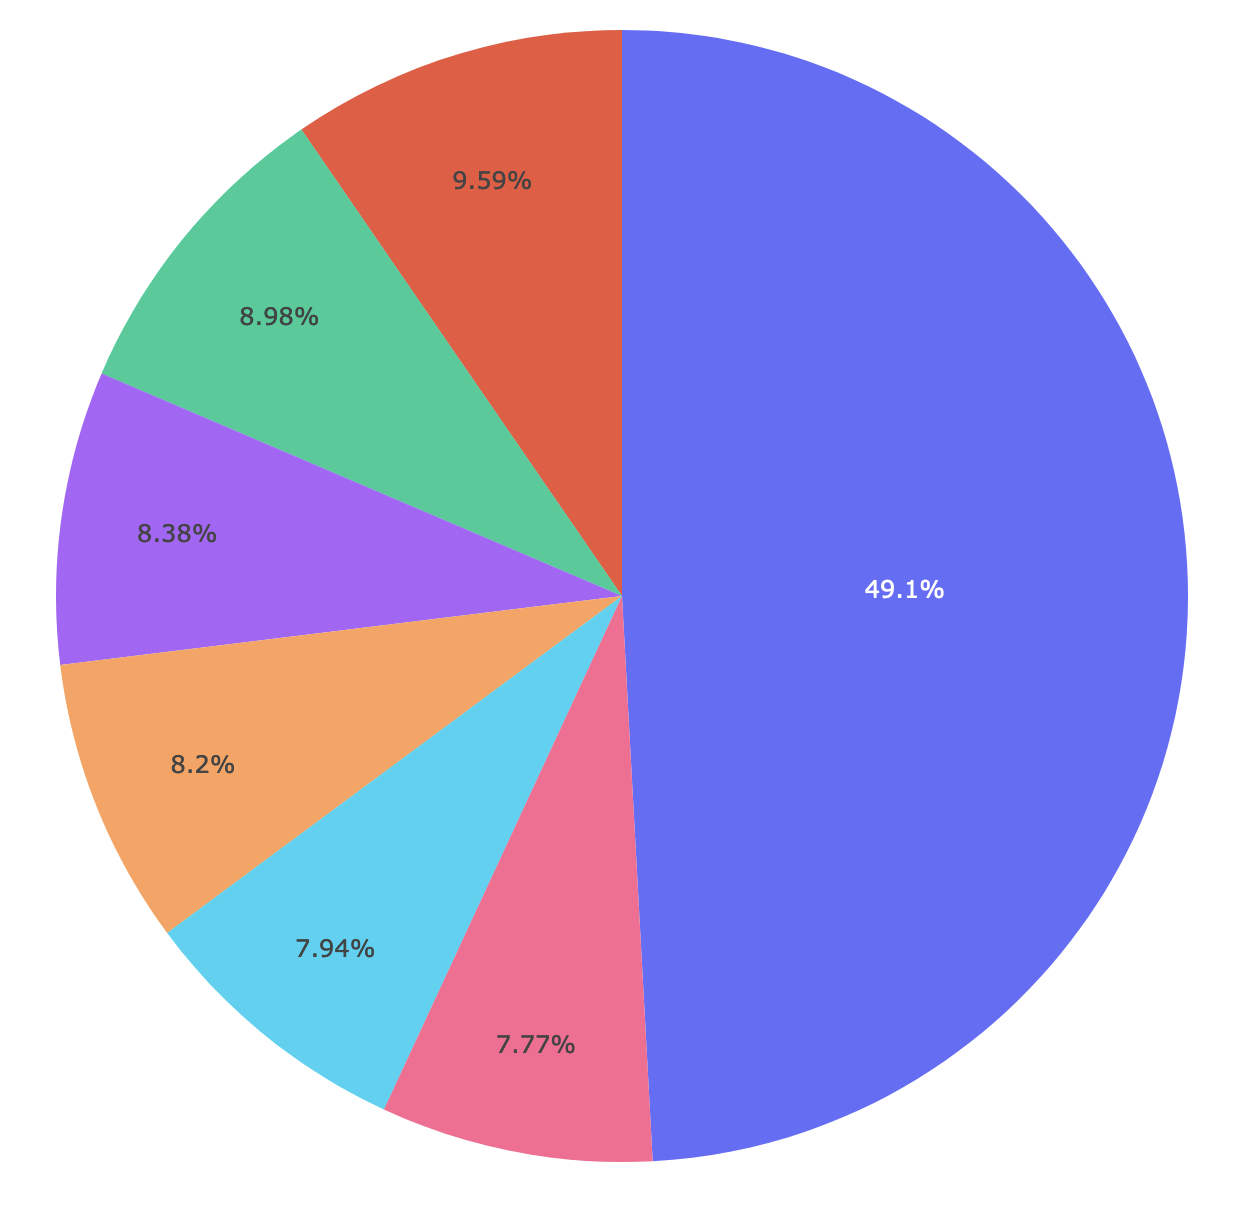
\includegraphics[width=\linewidth]{figures/no-emotion_context.png}
      \caption*{No emotion}
    \end{subfigure}\hfil
    \begin{subfigure}{0.19\textwidth}
      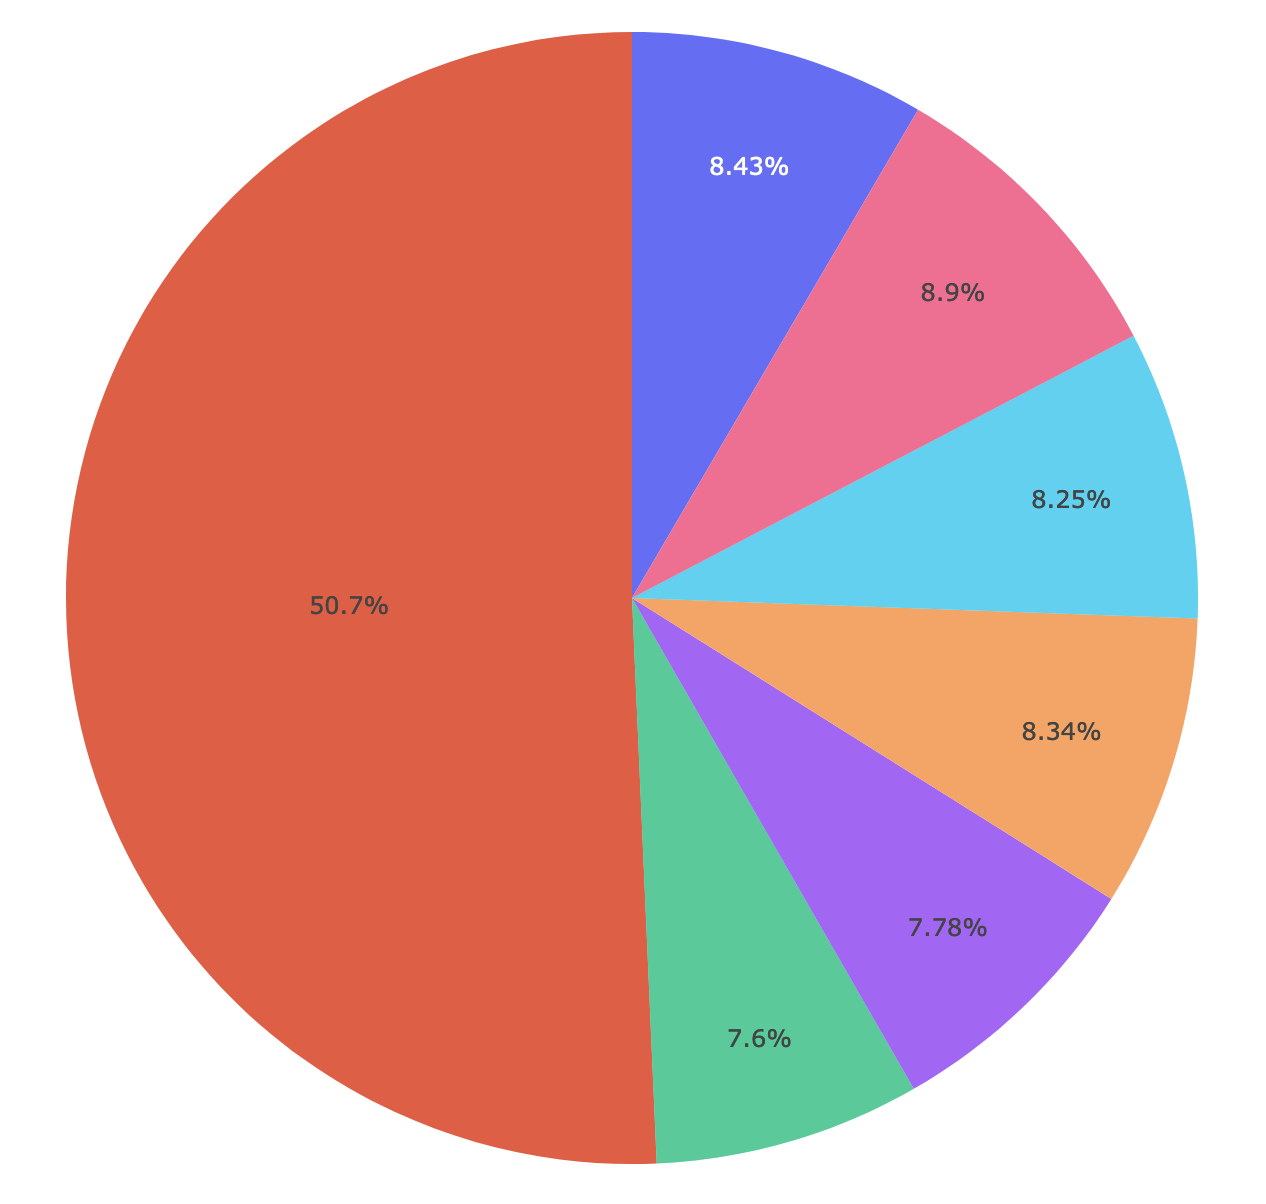
\includegraphics[width=\linewidth]{figures/anger_context.png}
      \caption*{Anger}
    \end{subfigure}\hfil
    \begin{subfigure}{0.19\textwidth}
      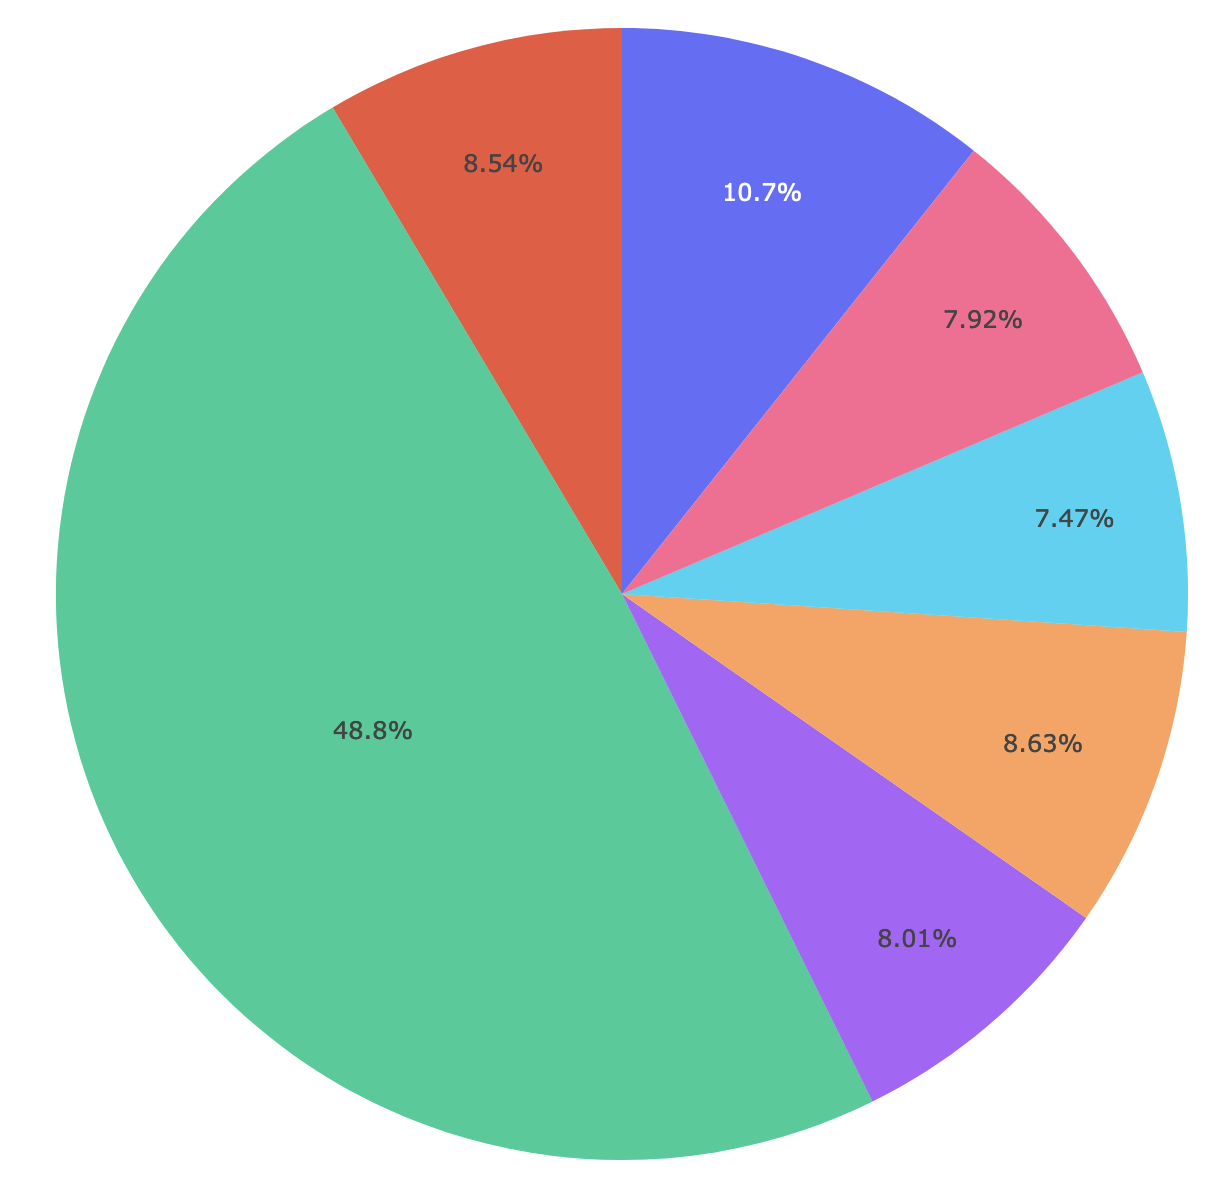
\includegraphics[width=\linewidth]{figures/disgust_context.png}
      \caption*{Disgust}
    \end{subfigure}\hfil
    \begin{subfigure}{0.19\textwidth}
      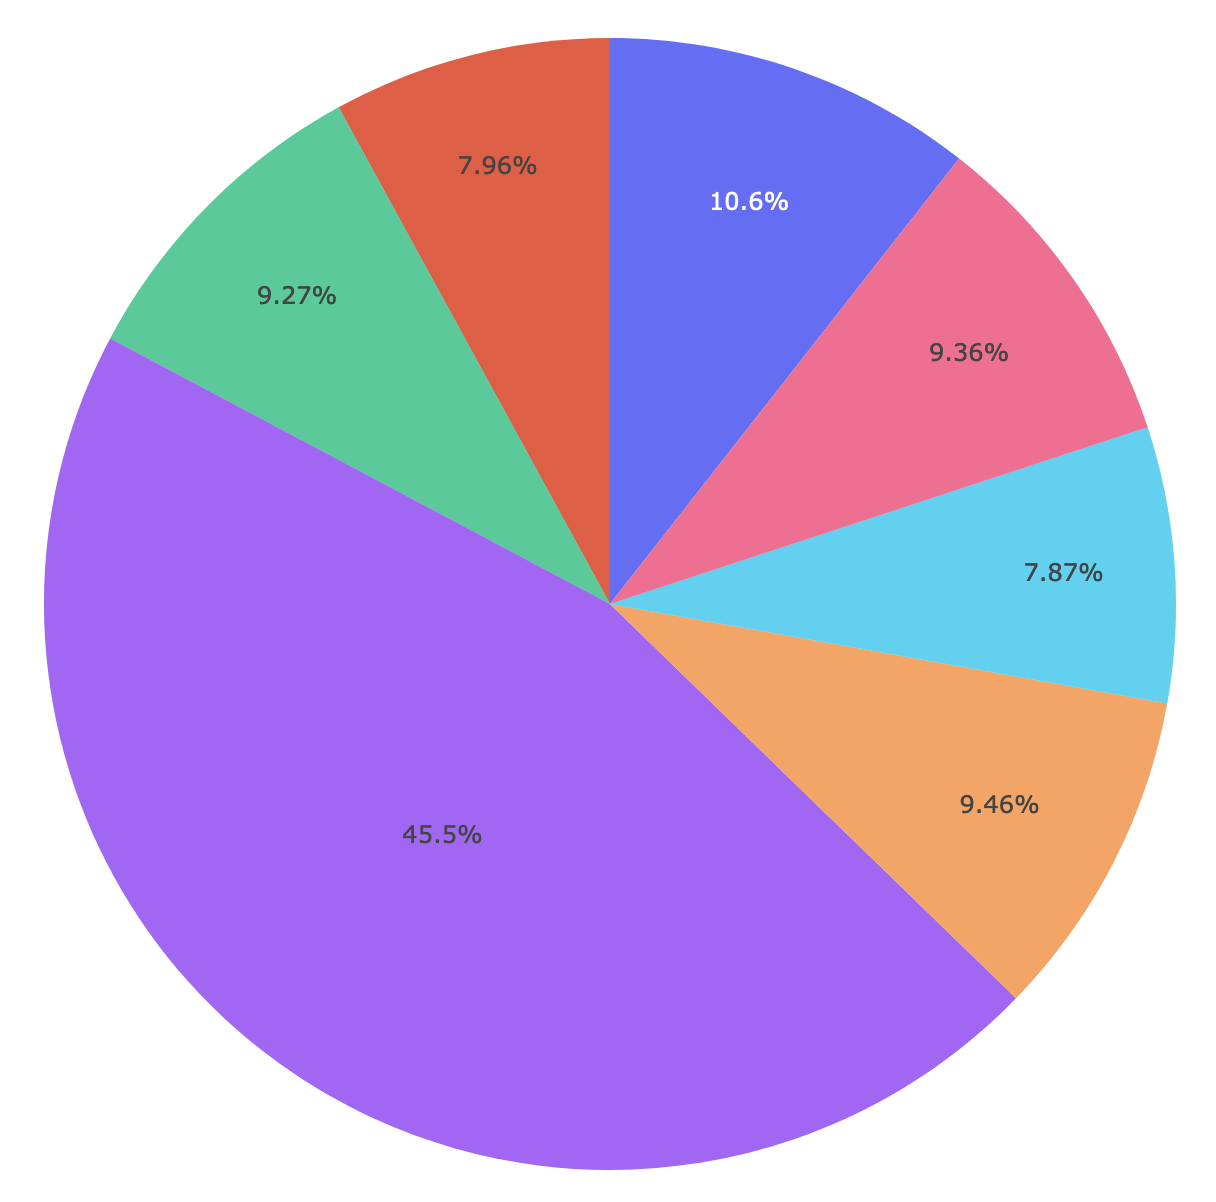
\includegraphics[width=\linewidth]{figures/fear_context.png}
      \caption*{Fear}
    \end{subfigure}
    
    \medskip
    \begin{subfigure}{0.19\textwidth}
      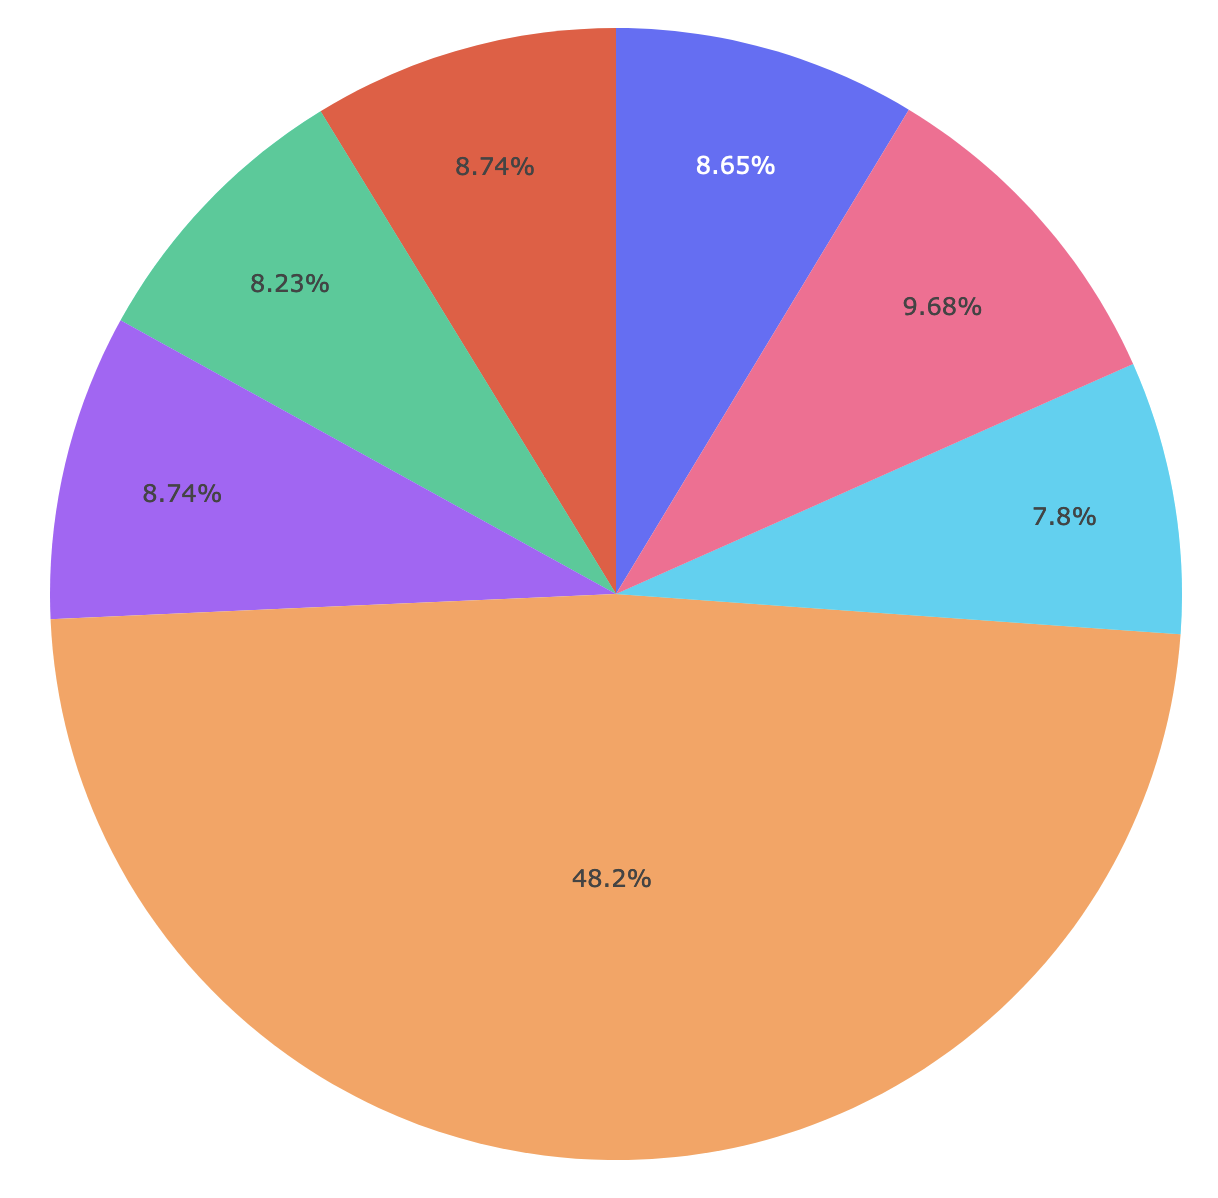
\includegraphics[width=\linewidth]{figures/happiness_context.png}
      \caption*{Happiness}
    \end{subfigure}\hfil 
    \begin{subfigure}{0.19\textwidth}
      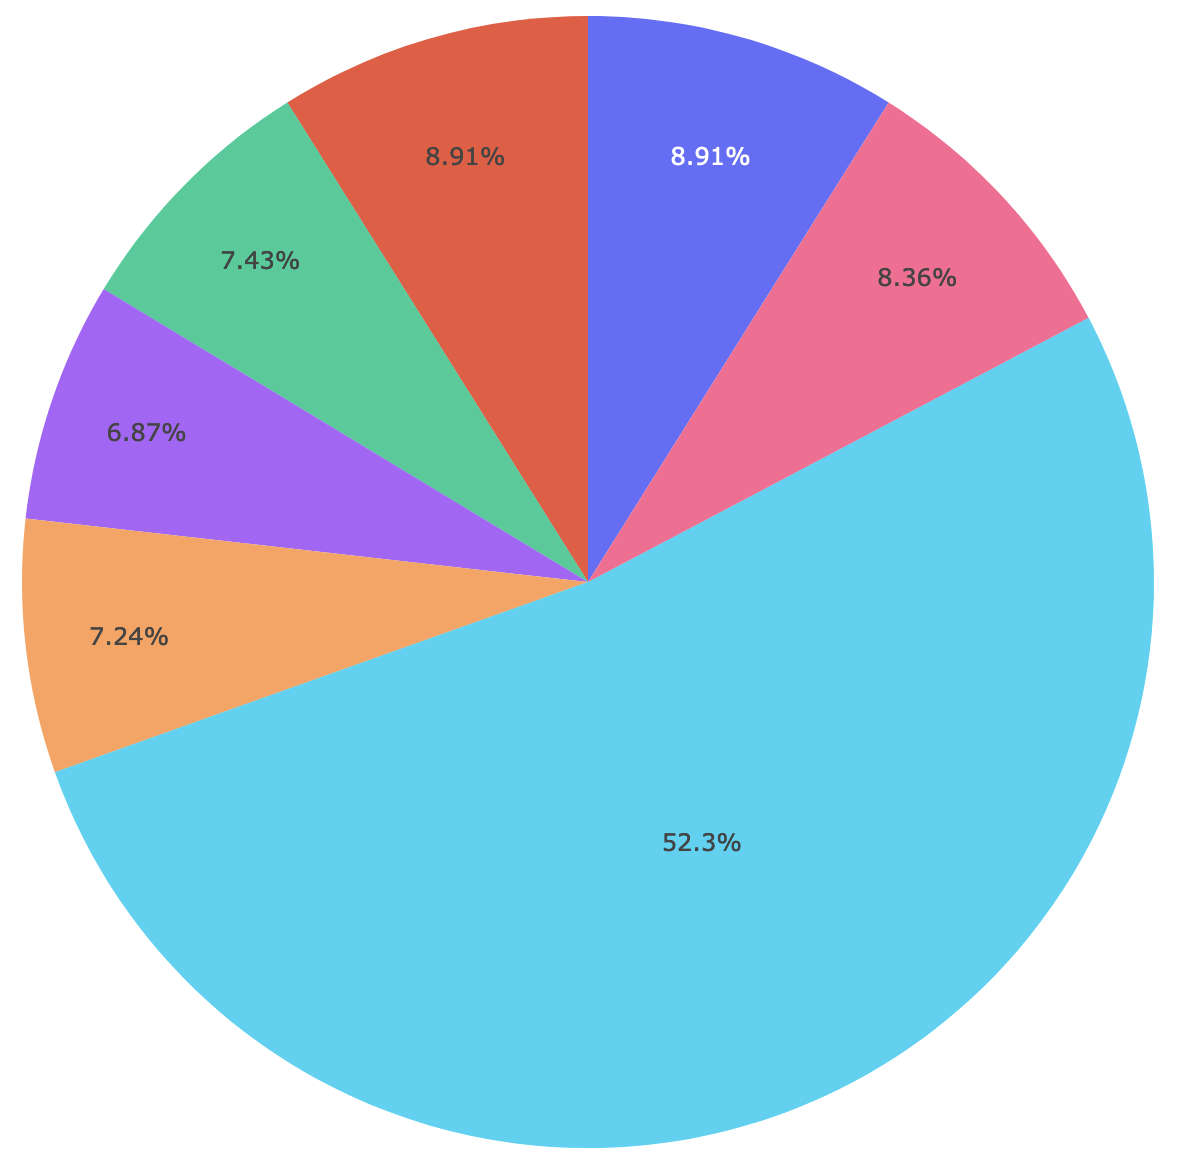
\includegraphics[width=\linewidth]{figures/sadness_context.png}
      \caption*{Sadness}
    \end{subfigure}\hfil 
    \begin{subfigure}{0.19\textwidth}
      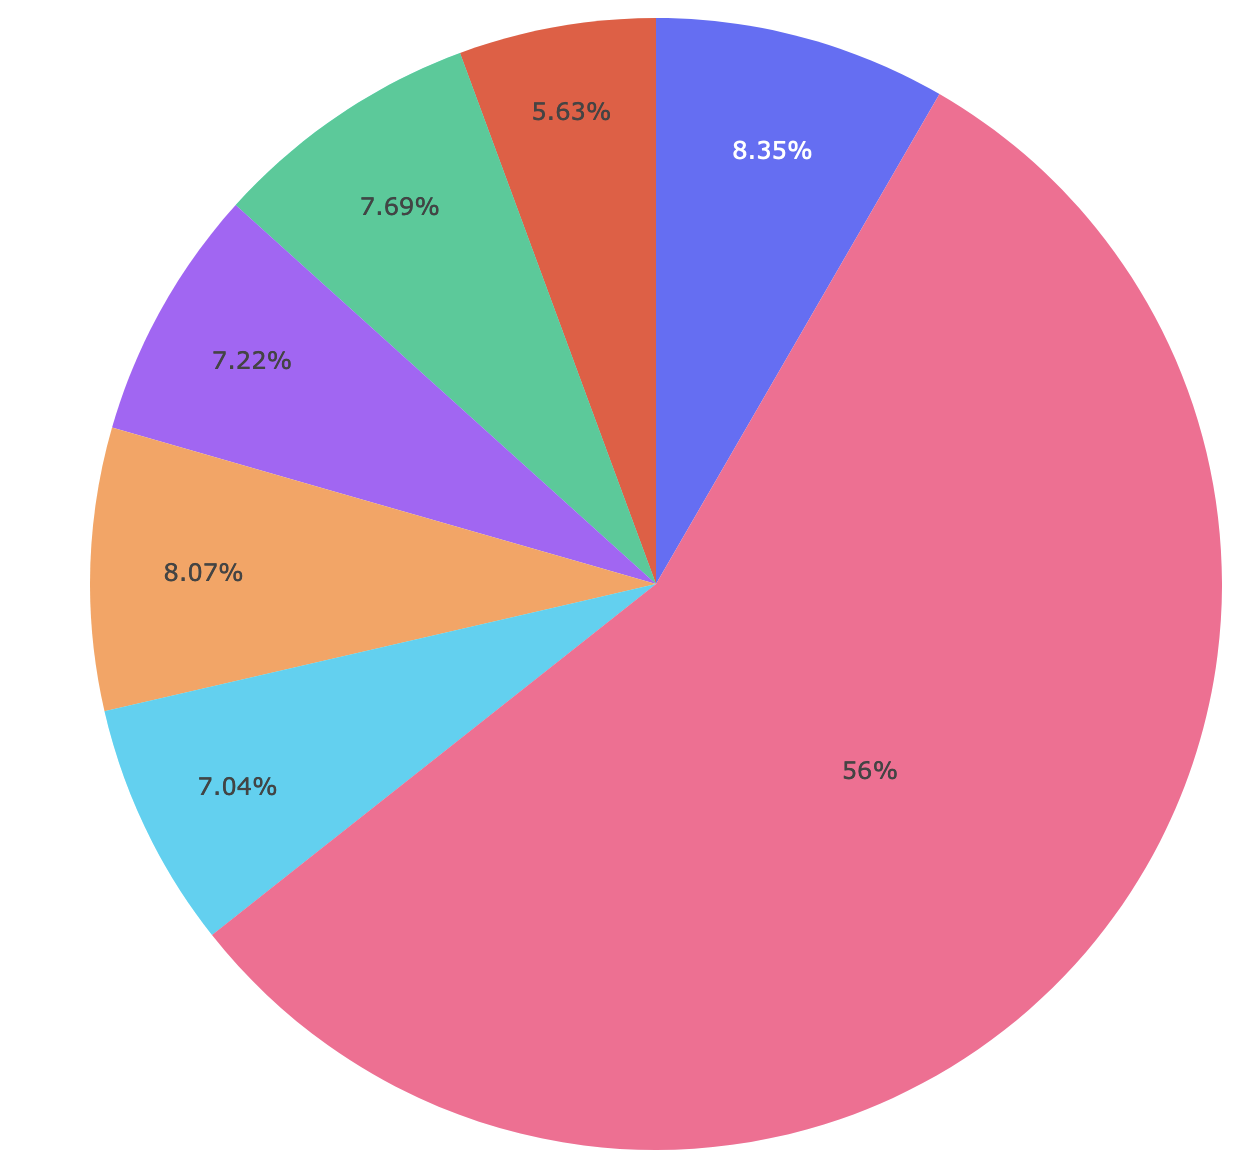
\includegraphics[width=\linewidth]{figures/surprise_context.png}
      \caption*{Surprise}
    \end{subfigure}\hfil
    \begin{subfigure}{0.19\textwidth}
      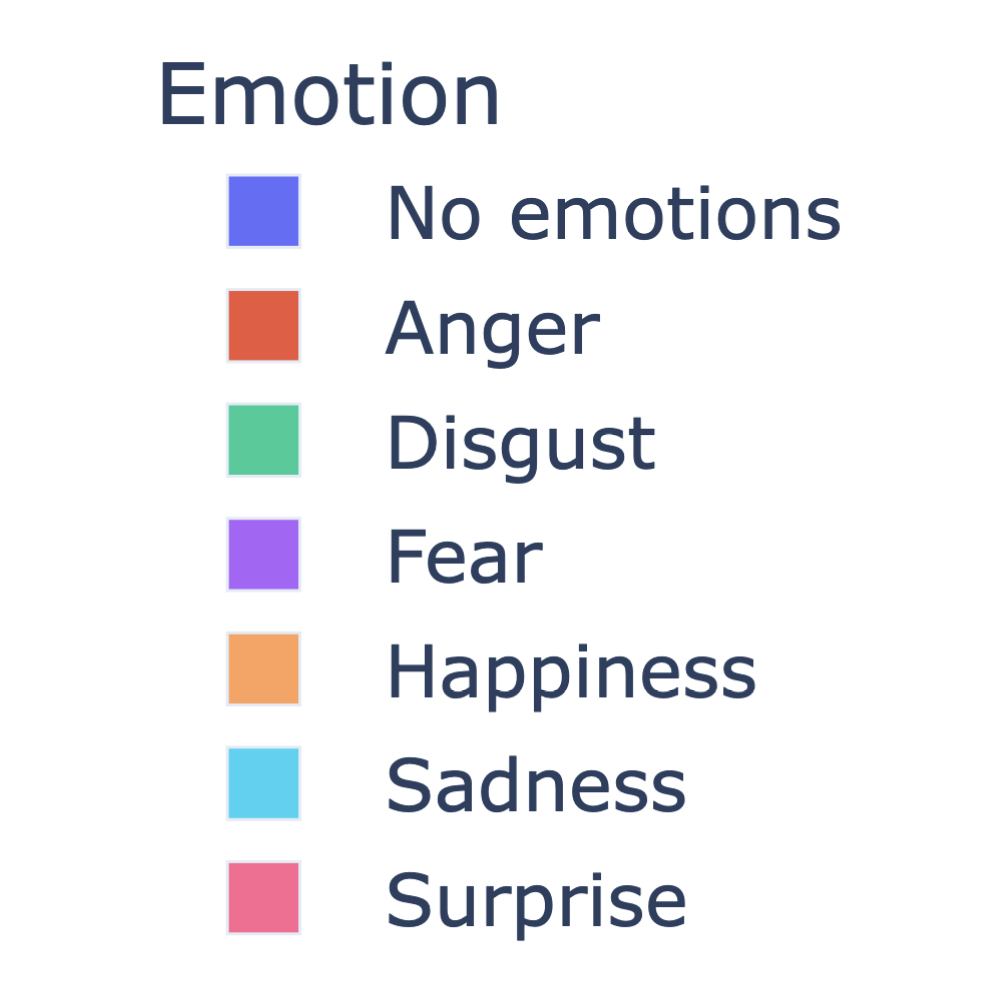
\includegraphics[width=\linewidth]{figures/legend.png}
      \caption*{}
    \end{subfigure}
    % \caption{\centering Distribution of predictions for each actual emotion in the case of contextual utterances representations.}
    \label{fig:pred_distrib_context}
    \end{figure}
    \end{frame}
    
    \begin{frame}[plain, noframenumbering]{Performances - Isolated Utterances}
        \begin{figure}
            \centering
            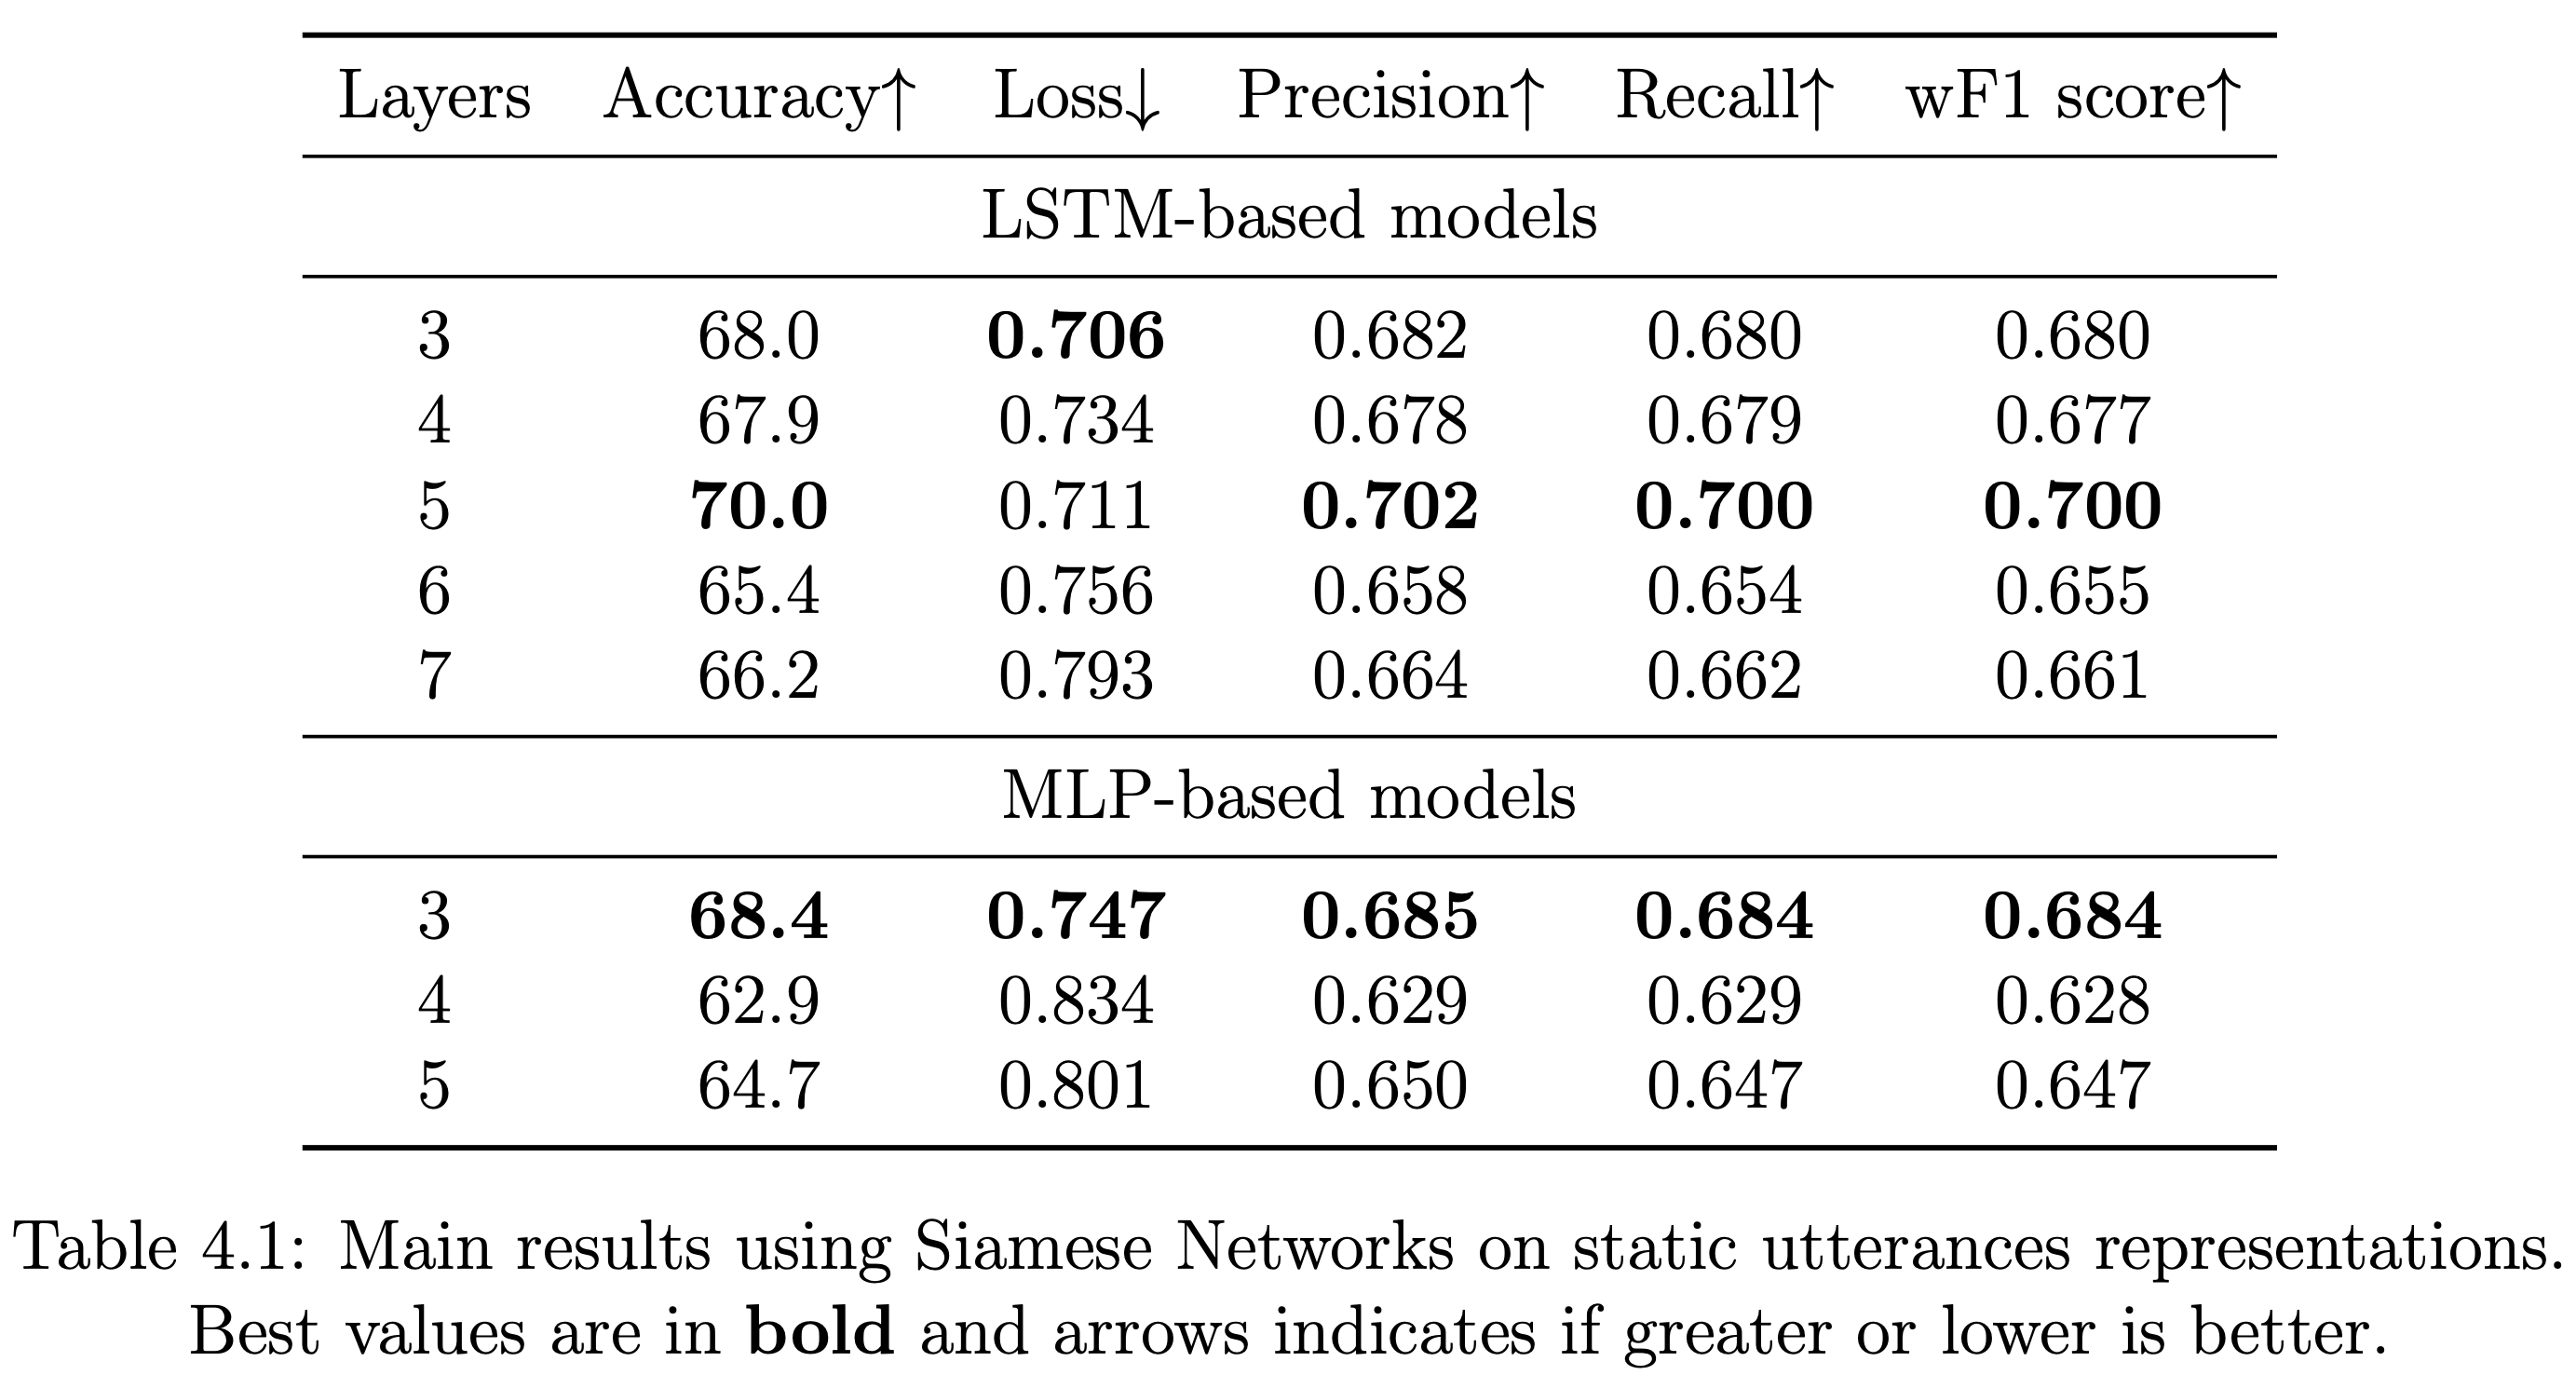
\includegraphics[width=0.9\textwidth]{figures/results_static_only.png}
            \label{fig:results_static}
        \end{figure}
    \end{frame}

\end{document}
